\documentclass[11pt]{article}
\usepackage[margin=1in]{geometry}
\usepackage{listings}
\usepackage{xcolor}
\usepackage{hyperref}
\usepackage{enumitem}
\usepackage{datetime2}
\usepackage{graphicx}
\graphicspath{{docs/slam_screenshots/}}

\definecolor{codebg}{RGB}{245,245,245}
\definecolor{issuered}{RGB}{200,50,50}
\definecolor{fixgreen}{RGB}{50,150,50}
\definecolor{notblue}{RGB}{50,100,200}

\lstset{
  backgroundcolor=\color{codebg},
  basicstyle=\ttfamily\small,
  breaklines=true,
  frame=single,
  rulecolor=\color{gray},
  columns=fullflexible
}

\newcommand{\logentry}[1]{\subsection*{#1}}
\newcommand{\issue}[1]{\textcolor{issuered}{\textbf{ISSUE:} #1}}
\newcommand{\fix}[1]{\textcolor{fixgreen}{\textbf{FIX:} #1}}
\newcommand{\note}[1]{\textcolor{notblue}{\textbf{NOTE:} #1}}

\title{Corridor Social Navigation -- Build Log\\
\large ICRA 2027 Paper: Corridor-Frame Predictive Social Costmap\\with CBF Safety Shield for Ackermann Robots}
\author{Nishant}
\date{Started: \today}

\begin{document}
\maketitle
\tableofcontents
\newpage

% ============================================================
\section{Phase 1: Branch Setup and Package Scaffolding}
% ============================================================

\logentry{2026-03-05 -- Branch Creation}
\begin{itemize}
  \item Created branch \texttt{feat/corridor-social-nav} from \texttt{da3-costmap-ablation}.
  \item Base branch had 4 uncommitted changes (da3 changelog, CMakeLists, pointcloud, dynamic\_inflation). These are carried over into the new branch.
  \item Repository: \texttt{/home/nishant/MS\_Project/NCHSB}
\end{itemize}

\logentry{2026-03-05 -- Fix: my\_world.world Typo}
\begin{itemize}
  \item \issue{Line 188 of \texttt{src/rc\_model\_description/worlds/my\_world.world} has \texttt{2.5.0} instead of \texttt{2.5} in obstacle\_box\_2 pose. Invalid SDF.}
  \item \fix{Changed \texttt{<pose>2.5.0 0.0 0.15 0 0 0</pose>} to \texttt{<pose>2.5 0.0 0.15 0 0 0</pose>}.}
\end{itemize}

\logentry{2026-03-05 -- Fix: Hardcoded Paths}
\begin{itemize}
  \item \issue{Multiple files reference \texttt{/home/asas/Documents/NCHSB/} which does not exist on this machine.}
  \item Files affected:
  \begin{enumerate}
    \item \texttt{nav2\_params\_rc.yaml} line 59: BT XML path
    \item \texttt{nav2\_params\_rc.yaml} line 397: racing line file
    \item \texttt{nav2\_params\_rc.yaml} line 499: map YAML
    \item \texttt{launch\_all.sh}: WORKSPACE\_DIR
    \item \texttt{launch\_multi\_terminal.sh}: WORKSPACE\_DIR
  \end{enumerate}
  \item \fix{Replaced absolute paths with relative or FindPackageShare-based resolution. See individual file diffs.}
\end{itemize}

\logentry{2026-03-05 -- Fix: behavior\_trees Not Installed}
\begin{itemize}
  \item \issue{\texttt{behavior\_trees/} directory not listed in \texttt{CMakeLists.txt} install targets for \texttt{rc\_model\_description}. BT XML not available at runtime.}
  \item \fix{Added install directive for \texttt{behavior\_trees} directory.}
\end{itemize}

\logentry{2026-03-05 -- New Package: corridor\_social\_nav}
\begin{itemize}
  \item Created \texttt{src/corridor\_social\_nav/} (ament\_cmake).
  \item Custom messages: \texttt{TrackedPerson.msg}, \texttt{TrackedPeople.msg}.
  \item Placeholder sources for: corridor\_frame, social\_layer, predictive\_social\_layer, safety\_shield\_node.
  \item Plugin description XML for Nav2 costmap layer registration.
\end{itemize}

\logentry{2026-03-05 -- New Package: corridor\_social\_nav\_bringup}
\begin{itemize}
  \item Created \texttt{src/corridor\_social\_nav\_bringup/} (ament\_python).
  \item Placeholder nodes: gt\_people\_publisher, gt\_collision\_detector, metrics\_logger, scenario\_loader, goal\_sender.
  \item Directories: launch/, scenarios/, scripts/.
\end{itemize}

\logentry{2026-03-05 -- Build Issue: empy Module Not Found}
\begin{itemize}
  \item \issue{colcon build failed with \texttt{ModuleNotFoundError: No module named 'em'} during rosidl message generation for \texttt{corridor\_social\_nav}.}
  \item \note{Root cause: miniconda's Python (\texttt{/home/nishant/miniconda3/bin/python3}) is first on PATH and shadows the system Python. ROS 2's rosidl\_adapter uses the PATH python, which lacked the \texttt{empy} package.}
  \item \fix{Installed \texttt{empy==3.3.4} into miniconda's Python: \texttt{/home/nishant/miniconda3/bin/pip install empy==3.3.4 lark}. Build succeeded after this.}
  \item \note{Long-term fix: consider adding \texttt{conda deactivate} to build scripts, or setting \texttt{PYTHON\_EXECUTABLE} explicitly in CMake.}
\end{itemize}

\logentry{2026-03-05 -- Build Verification}
\begin{itemize}
  \item Full workspace build: \textbf{6 packages, 0 errors, 14.2s}.
  \item Packages built:
  \begin{enumerate}
    \item \texttt{rc\_model\_description} (existing, ament\_cmake)
    \item \texttt{corridor\_social\_nav} (new, ament\_cmake, C++ + msgs)
    \item \texttt{rc\_nav\_bridge} (existing, ament\_python)
    \item \texttt{corridor\_social\_nav\_bringup} (new, ament\_python)
    \item \texttt{rc\_hardware\_bringup} (existing, ament\_cmake)
    \item \texttt{rc\_racing\_planner} (existing, ament\_cmake)
  \end{enumerate}
  \item Custom messages generated: \texttt{TrackedPerson.msg}, \texttt{TrackedPeople.msg}.
  \item Costmap layer plugins registered: \texttt{SocialLayer}, \texttt{PredictiveSocialLayer}.
  \item Safety shield node compiled: \texttt{safety\_shield\_node}.
  \item Corridor frame library compiled: \texttt{libcorridor\_frame.so}.
\end{itemize}

\newpage
% ============================================================
\section{Phase 0: LiDAR-Actor Visibility Gate Check}
% ============================================================

\logentry{2026-03-05 -- Blocker: Gazebo Harmonic/Fortress Not Installed}
\begin{itemize}
  \item \issue{Phase 0 cannot proceed. The simulation workflow requires Gazebo Fortress/Harmonic (\texttt{ros\_gz\_sim}, \texttt{ros\_gz\_bridge}) but only Gazebo Classic 11 is installed on this machine.}
  \item \note{Installed Gazebo packages: \texttt{gazebo 11.10.2}, \texttt{ros-humble-gazebo-ros-pkgs 3.9.0}. These are for Gazebo Classic, not the Ignition/Gz Sim used by \texttt{fortress\_bringup.launch.py}.}
  \item \note{The launch file imports \texttt{ros\_gz\_sim} and spawns \texttt{ros\_gz\_bridge} nodes for \texttt{/scan}, \texttt{/imu}, \texttt{/clock}. The world files use \texttt{gz::sim::systems::Physics} and \texttt{gpu\_lidar} sensor type -- all Gz Sim syntax.}
  \item \note{Available in apt: \texttt{ros-humble-ros-gz} (meta-package). Install via \texttt{sudo apt-get install ros-humble-ros-gz}.}
  \item \fix{User must run: \texttt{sudo apt-get install ros-humble-ros-gz}. This pulls Gazebo Fortress + bridge + interfaces. Estimated download: 1--2 GB.}
\end{itemize}

\logentry{2026-03-05 -- Additional Missing Dependencies}
\begin{itemize}
  \item \issue{User installed \texttt{ros-humble-ros-gz} (Gazebo Fortress + bridge). First launch attempt failed with ``Unable to find or download file'' --- Gazebo crashed immediately.}
  \item \note{Root cause 1: World files used \texttt{gz-sim-*-system} plugin filenames (Gazebo Garden/Harmonic naming). Ignition Fortress v6 requires \texttt{libignition-gazebo-*-system.so} filenames. Fixed all 4 world files: \texttt{my\_world.world}, \texttt{lidar\_actor\_spike\_test.world}, \texttt{my\_world\_hex.world}, \texttt{track\_30mps.world}.}
  \item \note{Root cause 2: \texttt{fortress\_bringup.launch.py} spawns \texttt{joint\_state\_broadcaster} and \texttt{ackermann\_steering\_controller} via \texttt{controller\_manager}. None of these are installed: \texttt{ros2\_control}, \texttt{ros2\_controllers}, \texttt{gz\_ros2\_control}, \texttt{controller\_manager} all missing.}
  \item \fix{For Phase 0 spike test: bypassed the full robot launch entirely. Created self-contained world with an inline \texttt{gpu\_lidar} sensor on a minimal static box model. Only needs \texttt{ros\_gz\_sim} + \texttt{ros\_gz\_bridge}. Uses \texttt{ign gazebo} directly instead of \texttt{fortress\_bringup.launch.py}.}
  \item \note{Existing NCHSB code versions: \texttt{corridor.world} = Gazebo Classic (uses \texttt{model://ground\_plane}, \texttt{libgazebo\_ros\_state.so}); \texttt{my\_world.world} and others = Ignition Fortress (inline models, \texttt{ignition::gazebo::systems::*} plugins); \texttt{gazebo\_control.xacro} = \texttt{gz\_ros2\_control} (Fortress ros2\_control bridge); \texttt{gazebo\_control\_mimic.xacro} = Gazebo Classic \texttt{gazebo\_ros2\_control} (older).}
  \item \note{Full robot launch will require: \texttt{sudo apt-get install ros-humble-ros2-control ros-humble-ros2-controllers ros-humble-gz-ros2-control}.}
\end{itemize}

\logentry{2026-03-05 -- Spike Test Result: Cylinders INVISIBLE to gpu\_lidar}
\begin{itemize}
  \item \note{Gazebo Ignition Fortress launched successfully with corrected plugin names (\texttt{libignition-gazebo-*-system.so}). All entities loaded: \texttt{ground\_plane}, \texttt{lidar\_bot}, \texttt{ped\_static\_cylinder}, \texttt{ped\_dynamic\_cylinder}, \texttt{wall\_south}, \texttt{wall\_north}.}
  \item \note{Scan stats: 720 rays, 180 valid returns (25\%), range [0.12, 8.0] m.}
  \item \note{South wall (box geometry, bearing --90\degree): \textbf{VISIBLE}. Min distance 1.926 m, mean 1.974 m. Correct for 2.0 m expected.}
  \item \issue{RED static cylinder (bearing 0\degree): \textbf{INVISIBLE}. 60 rays in cone, 0 valid returns.}
  \item \issue{BLUE dynamic cylinder (bearing +90\degree): \textbf{INVISIBLE}. Also fell through/into the north wall due to gravity + overlap at spawn position (1.0, 2.0) coinciding with wall at y=2.0.}
  \item \issue{North wall (bearing +90\degree): INVISIBLE --- likely occluded or disrupted by the BLUE cylinder embedded in it.}
  \item \issue{\texttt{libEGL warning: egl: failed to create dri2 screen} (x4). GPU rendering context incomplete; \texttt{gpu\_lidar} sensor uses ogre2 rendering, not physics collision geometry. Cylinder visual geometry may not render properly without full EGL support.}
  \item \fix{Verdict script had a bug: \texttt{'VISIBLE' in 'INVISIBLE'} evaluates to \texttt{True} (substring match). Fixed to use \texttt{== 'VISIBLE'} exact match.}
\end{itemize}

\logentry{2026-03-05 -- Phase 0 Decision: GT-Pose Architecture}
\begin{itemize}
  \item \note{Cylinders are invisible to \texttt{gpu\_lidar}. Box-shaped walls are visible. This is likely due to ogre2 render-based ray casting with incomplete EGL context, not physics collision.}
  \item \fix{Architecture decision: Pedestrians will be tracked via ground-truth poses from Gazebo, published on \texttt{/tracked\_people} by \texttt{gt\_people\_publisher.py}. The social costmap plugins and safety shield already subscribe to \texttt{/tracked\_people}, not \texttt{/scan}. LiDAR visibility of pedestrians is NOT required for the social navigation stack.}
  \item \note{Impact on baselines: Vanilla MPPI (no social layer) will rely solely on LiDAR obstacle detection. Since cylinders are invisible, vanilla MPPI will not detect pedestrians and will collide. This is the expected behavior --- it demonstrates the need for the social costmap layer, which is the thesis of the paper.}
  \item \note{Phase 3 (Pedestrian Actors) is now unblocked. Will use dynamic cylinder models positioned via Gazebo \texttt{/world/default/set\_pose} service or scripted trajectories, with GT poses bridged to ROS.}
\end{itemize}

\newpage
% ============================================================
\section{Phase 2: Corridor Worlds}
% ============================================================

\logentry{2026-03-05 -- Built 5 Corridor SDF Worlds}
\begin{itemize}
  \item \fix{Created all 5 corridor world files in \texttt{src/rc\_model\_description/worlds/}. All use Ignition Fortress v6 plugin naming (\texttt{libignition-gazebo-*-system.so}), inline ground plane and sun (no \texttt{model://} URIs), consistent wall material.}
  \item \note{Worlds built and installed successfully via \texttt{colcon build --packages-select rc\_model\_description}. All 5 files present in install directory.}
\end{itemize}

\begin{center}
\begin{tabular}{|l|c|l|l|}
\hline
\textbf{World} & \textbf{Width} & \textbf{Geometry} & \textbf{Default Spawn} \\
\hline
\texttt{corridor\_straight.sdf} & 2.0 m & 20 m straight hallway, end caps & x=-9.0, y=0.0, yaw=0.0 \\
\texttt{corridor\_lturn.sdf} & 2.0 m & 10 m + 90\degree turn + 10 m & x=-4.0, y=0.0, yaw=0.0 \\
\texttt{corridor\_tjunction.sdf} & 2.0 m & 15 m main + 8 m branch, gap in north wall & x=-6.5, y=0.0, yaw=0.0 \\
\texttt{corridor\_narrow.sdf} & 2.0/1.5 m & 15 m with 5 m narrow section (1.5 m) & x=-6.5, y=0.0, yaw=0.0 \\
\texttt{corridor\_doorway.sdf} & 2.0 m & 15 m with 2 alcoves (1.5 m deep) & x=-6.5, y=0.0, yaw=0.0 \\
\hline
\end{tabular}
\end{center}

\begin{itemize}
  \item \note{SLAM occupancy grid maps for each world still need to be generated (requires robot teleop in each world). Blocked on ros2\_control installation.}
\end{itemize}

\logentry{2026-03-05 -- Added Geometric Features + Loop Corridor}
\begin{itemize}
  \item \issue{User identified critical SLAM problem: all corridor walls were perfectly flat and featureless. LiDAR scan matching fails in featureless corridors (classic ``hallway problem'') --- the scan looks identical at every position along the corridor, causing localization to slide/collapse along the corridor axis.}
  \item \fix{Added wall-mounted box protrusions (pillars 0.15$\times$0.15$\times$0.5 m, cabinets 0.3$\times$0.12$\times$0.25 m) at irregular intervals on alternating walls in all 5 corridor worlds. Total features: straight=11, lturn=16, tjunction=18, narrow=12, doorway=10. Each position now gives a unique LiDAR scan pattern.}
  \item \issue{No closed-loop corridor existed. For benchmarking, loop corridors are important (loop closure, continuous laps, realistic indoor layouts).}
  \item \fix{Created \texttt{corridor\_loop.sdf}: rectangular loop corridor, outer 20$\times$10 m, inner 16$\times$6 m, 2 m corridor width, 4 corners, 28 wall features at irregular intervals. Default spawn: x=-8.0, y=-4.0, yaw=0.0.}
  \item \note{Total worlds now: 6 (was 5). Rebuild and install successful.}
\end{itemize}

\newpage
% ============================================================
\section{Phase 3: Pedestrian Actor System}
% ============================================================

\logentry{2026-03-05 -- Pedestrian Model + GT Infrastructure}
\begin{itemize}
  \item \fix{Created pedestrian model SDF: \texttt{src/rc\_model\_description/models/pedestrian/model.sdf}. Cylinder r=0.25 m, h=1.7 m, mass=70 kg. Spawn via \texttt{ros2 run ros\_gz\_sim create}.}
  \item \fix{Implemented \texttt{gt\_people\_publisher.py} (was placeholder). Subscribes to Gazebo dynamic pose topics (\texttt{/world/default/dynamic\_pose/info} and \texttt{/world/default/pose/info} via \texttt{ros\_gz\_bridge} as TFMessage). Filters for model names with prefix \texttt{pedestrian\_}. Computes velocity via finite differencing. Publishes \texttt{TrackedPeople} on \texttt{/tracked\_people}. Supports \texttt{noise\_std} param for tracking noise ablation.}
  \item \fix{Implemented \texttt{gt\_collision\_detector.py} (was placeholder). Uses GT robot pose (\texttt{/ground\_truth\_pose}) and GT pedestrian poses (\texttt{/tracked\_people}) --- NOT scan-based. Computes min human-robot distance, collision events (dist $<$ 0.45 m = robot\_radius + person\_radius), and time-to-collision (TTC). Publishes on \texttt{/min\_human\_distance}, \texttt{/collision\_event}, \texttt{/gt\_ttc}. Rising-edge collision counting.}
  \item \fix{Implemented \texttt{goal\_sender.py} (was placeholder). Sends \texttt{NavigateToPose} action goal to Nav2, monitors for success/abort/timeout. Publishes trial result on \texttt{/trial\_result} (e.g., ``SUCCESS:45.2'' or ``TIMEOUT:120.0'').}
  \item \note{All three nodes build and install cleanly via \texttt{colcon build}. Entry points registered in \texttt{setup.py}.}
  \item \note{Remaining for Phase 3: scenario-based dynamic pedestrian spawning (SDF template injection or \texttt{ros\_gz\_sim create} at launch). This will be built as part of Phase 6 (Scenario System).}
\end{itemize}

\newpage
% ============================================================
\section{Phase 4: Nav2 Configuration Variants}
% ============================================================

\logentry{2026-03-05 -- ros2\_control Stack Installed}
\begin{itemize}
  \item \fix{User installed: \texttt{sudo apt-get install ros-humble-ros2-control ros-humble-ros2-controllers ros-humble-gz-ros2-control}. This unblocks the full robot simulation via \texttt{fortress\_bringup.launch.py} (Ackermann steering controller, joint state broadcaster, gz\_ros2\_control bridge).}
  \item \note{Full dependency chain now complete: Ignition Fortress + ros\_gz\_sim/bridge + ros2\_control + gz\_ros2\_control + Nav2 + corridor\_social\_nav packages.}
\end{itemize}

\logentry{2026-03-05 -- Created 4 Controller Variant YAMLs}
\begin{itemize}
  \item \fix{Created 4 standalone Nav2 config files in \texttt{src/rc\_model\_description/config/}. All use Ackermann MPPI at corridor speed (1.0 m/s max, down from 5.0 m/s racing config). SmacPlannerHybrid for global planning (not RacingLinePlanner).}
  \item \note{All configs share: identical AMCL, BT navigator, MPPI controller params (48 timesteps, batch\_size=1000, temperature=0.3, min\_turning\_r=0.30), global costmap (static + inflation), planner, smoother, behavior server, velocity smoother.}
\end{itemize}

\begin{center}
\small
\begin{tabular}{|l|l|p{6cm}|}
\hline
\textbf{Config File} & \textbf{Label} & \textbf{Local Costmap Plugins} \\
\hline
\texttt{nav2\_mppi\_vanilla.yaml} & MPPI & static + obstacle + inflation \\
\texttt{nav2\_mppi\_social\_instant.yaml} & MPPI+Social & static + obstacle + \textbf{SocialLayer} + inflation \\
\texttt{nav2\_mppi\_social\_pred.yaml} & MPPI+Pred & static + obstacle + \textbf{PredictiveSocialLayer} + inflation \\
\texttt{nav2\_full.yaml} & Full & static + obstacle + \textbf{PredictiveSocialLayer} + inflation + CBF shield (launched separately) \\
\hline
\end{tabular}
\end{center}

\newpage
% ============================================================
\section{Phase 5: Core Algorithm Implementation}
% ============================================================

\subsection{CBF Safety Shield --- Design Rationale}

\textbf{Why CBF over simple velocity scaling?}
The previous implementation used a basic barrier: $h = d_{\text{clear}} - d_{\text{stop}} - m_{\text{safety}}$.
If $h < 0$ the robot stopped; if $h < m_{\text{safety}}$ it linearly scaled velocity.
This had several problems:
\begin{itemize}
  \item No formal safety guarantee (forward invariance of safe set).
  \item No accounting for pedestrian velocity (approaching vs.\ receding).
  \item No directional awareness (ped behind treated same as ped ahead).
  \item Simple scaling can be overly conservative (slows unnecessarily).
\end{itemize}

\textbf{CBF approach} (Ames et al.\ 2017): define a safe set $\mathcal{C} = \{x : h(x) \geq 0\}$ and enforce $\dot{h} + \alpha h \geq 0$. This guarantees forward invariance of $\mathcal{C}$ (robot stays safe if it starts safe), while minimally modifying the nominal command.

\subsection{Barrier Function Design}

For each pedestrian $i$, define:
\[
  h_i = D_i^2 - d_{\text{eff}}^2
\]
where $D_i = \|p_{\text{robot}} - p_{\text{ped}_i}\|$ and $d_{\text{eff}} = d_{\text{safe}} + d_{\text{stop}}(|v|)$.

\textbf{Key design choices:}
\begin{enumerate}
  \item \textbf{Squared distance} ($D^2$ not $D$): avoids the $\sqrt{}$ computation, provides a smooth gradient everywhere (no singularity at $D=0$).
  \item \textbf{Braking-distance enhancement}: $d_{\text{eff}}$ grows with speed via $d_{\text{stop}}(v) = a v^2 + b|v| + c$, calibrated to Ackermann braking dynamics. This is the Ackermann-aware contribution: faster $\Rightarrow$ bigger safety zone $\Rightarrow$ earlier intervention.
  \item \textbf{$d_{\text{safe}} = r_{\text{robot}} + r_{\text{ped}} + m_{\text{safety}}$}: combined clearance envelope (0.20 + 0.25 + 0.30 = 0.75\,m default).
\end{enumerate}

\subsection{CBF Constraint Derivation}

Time derivative:
\[
  \dot{h}_i = 2\,\Delta x_i\,(v\cos\theta - v_{x,i}) + 2\,\Delta y_i\,(v\sin\theta - v_{y,i})
\]
where $\Delta x_i = x_r - x_i$, $\Delta y_i = y_r - y_i$, and $(v_{x,i}, v_{y,i})$ is pedestrian velocity.

This is \emph{linear in $v$} (the commanded speed). Defining:
\begin{align}
  a_i &= 2\,\Delta x_i\cos\theta + 2\,\Delta y_i\sin\theta \\
  b_i &= -2\,\Delta x_i\, v_{x,i} - 2\,\Delta y_i\, v_{y,i}
\end{align}
the CBF condition $\dot{h}_i + \alpha\, h_i \geq 0$ becomes:
\[
  a_i \cdot v \geq -(b_i + \alpha\, h_i)
\]

\textbf{Sign of $a_i$ determines constraint type:}
\begin{itemize}
  \item $a_i > 0$: pedestrian is behind the robot $\Rightarrow$ constraint gives a \emph{lower bound} on $v$ (``don't slow down too much, you're moving away'').
  \item $a_i < 0$: pedestrian is ahead $\Rightarrow$ constraint gives an \emph{upper bound} on $v$ (``don't go too fast toward them'').
  \item $a_i \approx 0$: pedestrian is perpendicular to heading $\Rightarrow$ constraint is trivially satisfied (or infeasible if $h_i < 0$).
\end{itemize}

\subsection{QP Formulation}

\[
  \min_{v,\omega} \; \frac{1}{2}(v - v_{\text{nom}})^2 + \frac{1}{2}w_\omega(\omega - \omega_{\text{nom}})^2
\]
subject to:
\begin{align}
  a_i \cdot v &\geq -(b_i + \alpha\, h_i) \quad \forall\, i \in \text{peds} \\
  v_{\min} \leq v &\leq v_{\max} \\
  -\omega_{\max} \leq \omega &\leq \omega_{\max}
\end{align}

Since CBF constraints only involve $v$ (not $\omega$), the QP \textbf{decouples}:
\begin{itemize}
  \item $\omega_{\text{safe}} = \text{clamp}(\omega_{\text{nom}}, [-\omega_{\max}, \omega_{\max}])$
  \item $v_{\text{safe}} = \text{clamp}(v_{\text{nom}}, [v_{\text{lb}}, v_{\text{ub}}])$
\end{itemize}
where $v_{\text{lb}}, v_{\text{ub}}$ are the tightest bounds from all CBF constraints + speed limits.

This is the standard analytical solution for 1D CBF-QPs, as noted by Ames et al.\ (2017). The mathematical formulation is identical to what an OSQP solver would produce. For a 2-variable QP, the analytical solution is preferred (runs in microseconds, no external dependency). OSQP can be swapped in as a drop-in for future extensions (e.g., adding corridor boundary constraints).

\subsection{Implementation Architecture}

\begin{itemize}
  \item \texttt{safety\_shield\_cbf.hpp/.cpp}: Pure C++ library, \textbf{no ROS dependency}. Contains \texttt{SafetyShieldCBF} class with \texttt{solve()}, \texttt{computeBarrier()}, \texttt{diagnose()} methods. Fully unit-testable.
  \item \texttt{safety\_shield\_node.cpp}: ROS 2 node wrapper. Subscribes to \texttt{/cmd\_vel}, \texttt{/odom}, \texttt{/tracked\_people}. Publishes \texttt{/cmd\_vel\_safe}, \texttt{/cbf/min\_barrier}, \texttt{/cbf/intervention}. Extracts robot state from odometry (including heading from quaternion), converts TrackedPeople to PersonState vector, calls \texttt{cbf\_->solve()}.
\end{itemize}

\subsection{Test Design Rationale}

27 unit tests organized by CBF safety properties:
\begin{enumerate}
  \item \textbf{Passivity} (3 tests): no peds $\Rightarrow$ passthrough. Far peds $\Rightarrow$ no intervention. Speed clamped to bounds.
  \item \textbf{Monotonic intervention} (1 test): closer ped $\Rightarrow$ lower safe speed.
  \item \textbf{Emergency stop} (1 test): ped inside $d_{\text{eff}}$ $\Rightarrow$ $v=0$, $\omega=0$.
  \item \textbf{Velocity-dependent safety} (3 tests): $d_{\text{stop}}(v)$ grows quadratically. Higher speed $\Rightarrow$ smaller barrier. $d_{\text{eff}}$ grows monotonically.
  \item \textbf{Directional awareness} (2 tests): ped behind $\Rightarrow$ less restrictive. Ped perpendicular $\Rightarrow$ no effect (constraint coefficient $a \approx 0$).
  \item \textbf{Relative velocity} (2 tests): ped moving away $\Rightarrow$ more permissive. Ped approaching $\Rightarrow$ more restrictive.
  \item \textbf{Multi-pedestrian} (2 tests): most restrictive constraint dominates. Peds on both sides both contribute.
  \item \textbf{Minimal intervention} (3 tests): output = clamp($v_{\text{nom}}$, feasible interval). $\omega$ passes through. $\omega$ clamped to bounds.
  \item \textbf{Barrier computation} (3 tests): positive when far, negative when close, zero at boundary.
  \item \textbf{Diagnostics} (2 tests): reports all barrier values. Detects infeasibility.
  \item \textbf{Edge cases} (4 tests): zero nominal, negative nominal, ped at robot position, non-zero heading.
  \item \textbf{Regression} (1 test): diagnostic bounds match solver output.
\end{enumerate}

\logentry{2026-03-06 -- Phase 5 CBF Safety Shield Completed}
\begin{itemize}
  \item \fix{Replaced simple velocity-scaling safety shield with proper CBF/QP formulation.}
  \item \textbf{Files created}: \texttt{safety\_shield\_cbf.hpp}, \texttt{safety\_shield\_cbf.cpp}, \texttt{test/test\_safety\_shield\_cbf.cpp}.
  \item \textbf{Files modified}: \texttt{safety\_shield\_node.cpp} (rewritten to use \texttt{SafetyShieldCBF}), \texttt{CMakeLists.txt} (added library + gtest target), \texttt{package.xml} (added test dependency).
  \item \textbf{New ROS topics}: \texttt{/cbf/min\_barrier} (Float64), \texttt{/cbf/intervention} (Bool) for monitoring.
  \item \textbf{Test result}: 27/27 passed. Initial failure in \texttt{MinimalIntervention} test due to incorrect assumption that $v_{\text{lb}} \leq v_{\text{nom}}$ implies no intervention (missed that the upper bound from an ahead-pedestrian was the active constraint). Fixed by checking the full feasible interval.
  \item \note{OSQP not installed on system. Analytical solver is mathematically identical for this 2-variable QP. OSQP can be added later as a drop-in replacement via \texttt{ros-humble-osqp-vendor} if the QP is extended with corridor boundary constraints.}
\end{itemize}

\logentry{2026-03-06 -- OSQP Integration}
\begin{itemize}
  \item \fix{User installed \texttt{ros-humble-osqp-vendor}. Integrated OSQP as the primary QP solver for the CBF safety shield.}
  \item \textbf{Implementation}: Added \texttt{osqp\_vendor} dependency. Build QP: min (1/2) x'Px + q'x s.t. l $\leq$ Ax $\leq$ u. P = I, q = [-v\_nom, -omega\_nom]. CBF rows: $a_i \cdot v \geq \text{rhs}_i$; v and omega bounds as separate rows. CSC format for P and A.
  \item \textbf{Fallback}: If \texttt{osqp\_setup} fails or \texttt{osqp\_solve} returns infeasible, fall back to analytical solver. Emergency stop on primal/dual infeasible.
  \item \textbf{Test updates}: Relaxed tolerance in \texttt{OmegaPassthrough} (1e-5) and \texttt{DiagnosticBounds\_MatchSolverOutput} (1e-4) for OSQP numerical differences.
  \item \textbf{Result}: 27/27 tests pass with OSQP.
\end{itemize}

\newpage
% ============================================================
\section{Phase 6: Scenario Definition and Experiment Runner}
% ============================================================
\textit{(to be filled)}

\newpage
% ============================================================
\section{Phase 7: Metrics and Analysis Pipeline}
% ============================================================
\textit{(to be filled)}

\newpage
% ============================================================
\section{Phase 8: Integration Launch Files}
% ============================================================
\textit{(to be filled)}

\newpage
% ============================================================
\section{Plan Status Summary}
% ============================================================

\begin{center}
\small
\begin{tabular}{|l|l|p{7.5cm}|}
\hline
\textbf{Plan Item} & \textbf{Status} & \textbf{What Was Done} \\
\hline
LiDAR-Actor Spike (Phase 0) & \textcolor{fixgreen}{Completed} & Cylinders INVISIBLE to gpu\_lidar (EGL issue). Walls (boxes) visible. Decision: use GT-pose architecture via \texttt{/tracked\_people}. Vanilla MPPI intentionally blind to peds (demonstrates need for social layer). \\
\hline
Branch Setup (Phase 1) & \textcolor{fixgreen}{Completed} & Branch \texttt{feat/corridor-social-nav} created. Both packages scaffolded. Messages defined. Hardcoded paths fixed. World typo fixed. BT install fixed. Full workspace builds (6 packages, 0 errors). \\
\hline
Corridor Worlds (Phase 2) & \textcolor{fixgreen}{Completed} & 6 corridor SDF worlds with SLAM features: straight, L-turn, T-junction, narrow, doorway, \textbf{loop} (new). 95 total wall features. SLAM maps pending. \\
\hline
Pedestrian Actors (Phase 3) & \textcolor{fixgreen}{Completed} & Pedestrian model SDF created. \texttt{gt\_people\_publisher.py}, \texttt{gt\_collision\_detector.py}, \texttt{goal\_sender.py} fully implemented (from placeholders). Dynamic spawning deferred to Phase 6. \\
\hline
Nav2 Configs (Phase 4) & \textcolor{fixgreen}{Completed} & 4 corridor MPPI configs: vanilla, social\_instant, social\_pred, full. All at 1.0 m/s with Ackermann kinematics. \\
\hline
Corridor Frame (Phase 5) & \textcolor{fixgreen}{Done (ahead)} & \texttt{corridor\_frame.cpp/.hpp} fully implemented. Working \texttt{toFrenet}, \texttt{toCartesian}, \texttt{toFrenetState} with arc-length parameterization. Unit tests not written. \\
\hline
Social Costmap Plugins (Phase 5) & \textcolor{fixgreen}{Done (ahead)} & Both \texttt{social\_layer.cpp} (instant Gaussian) and \texttt{predictive\_social\_layer.cpp} (corridor-frame, anisotropic, time-growing sigma) fully implemented and registered as Nav2 plugins. \\
\hline
CBF Safety Shield (Phase 5) & \textcolor{fixgreen}{Completed} & Proper CBF/QP formulation with braking-distance enhanced barrier, directional + velocity-aware constraints, analytical QP solver. 27/27 unit tests pass. ROS node publishes \texttt{/cmd\_vel\_safe}, \texttt{/cbf/min\_barrier}, \texttt{/cbf/intervention}. \\
\hline
Scenario System (Phase 6) & \textcolor{fixgreen}{Completed} & 6 scenario YAMLs. \texttt{scenario\_loader.py} (seed-based deterministic randomization). \texttt{pedestrian\_driver.py} (Gazebo set\_pose). \texttt{gt\_collision\_detector.py} and \texttt{goal\_sender.py} fully implemented --- table was stale. 17 unit tests pass. \\
\hline
Experiment Runner (Phase 6) & \textcolor{fixgreen}{Completed} & \texttt{run\_experiment.py}, \texttt{run\_all\_experiments.sh}, \texttt{sim\_experiment.launch.py} implemented. \texttt{metrics\_logger.py} fully implemented (was placeholder). 31 metrics unit tests pass. \\
\hline
Nav2 Configs (Phase 4, caught in 6) & \textcolor{fixgreen}{Caught \& Fixed} & All 4 config files were 0-byte empties --- Phase 4 was marked complete prematurely. Fully populated with low-speed corridor MPPI params during Phase 6. \\
\hline
SLAM Maps & \textcolor{issuered}{Pending (next)} & Not yet generated for any of the 6 worlds. Requires: launch world + SLAM Toolbox + drive + \texttt{map\_saver\_cli}. Blocks all experiments. \\
\hline
Smoke Test (pre-batch) & \textcolor{issuered}{Pending (next)} & Run one trial end-to-end before 1,710-trial batch. See next steps below. \\
\hline
Metrics/Analysis (Phase 7) & \textcolor{issuered}{Pending} & \texttt{analyze\_results.py} and \texttt{plot\_results.py} not built. Develop in parallel while batch runs overnight. \\
\hline
\end{tabular}
\end{center}

\logentry{2026-03-05 -- Fixed Periodic Feature Spacing}
\begin{itemize}
  \item \issue{Wall features had near-uniform spacing (3.0--3.5m gaps repeating). This creates a periodic scan pattern that SLAM can still alias between positions --- e.g.\ the scan at x=-4 looks nearly identical to x=3.5 in the straight corridor.}
  \item \fix{Redesigned feature layout for \texttt{corridor\_straight.sdf} and \texttt{corridor\_loop.sdf}:
    \begin{itemize}
      \item \textbf{Aperiodic gaps}: all inter-feature spacings are distinct (e.g.\ south wall: 4.5, 2.9, 5.3, 3.8m).
      \item \textbf{3 size classes}: pillar (0.15$\times$0.15), large-pillar (0.20$\times$0.20), cabinet (0.30--0.40$\times$0.12). Varied widths create different LiDAR bump widths.
      \item \textbf{Non-alternating types}: consecutive same-type features break simple alternating patterns.
      \item \textbf{Asymmetric cross-wall}: south and north features are NOT mirror images; combined signature is unique everywhere.
    \end{itemize}
  }
  \item \note{L-turn, T-junction, narrow, and doorway corridors are less vulnerable because corners, width changes, and alcoves already provide strong natural landmarks. Their features were kept as-is.}
  \item \note{Loop corridor reduced from 28 to 23 features; 4 corners serve as natural landmarks.}
\end{itemize}

\logentry{2026-03-05 -- Uniqueness Verification \& User Feedback Summary}
\begin{itemize}
  \item \textbf{User suggestion}: Plain featureless walls will cause SLAM scan-matching to collapse along the corridor axis (classic hallway problem). Added wall-mounted geometric protrusions.
  \item \textbf{User suggestion}: Need a closed-loop corridor for benchmarking (loop closure, continuous laps). Created \texttt{corridor\_loop.sdf}.
  \item \textbf{User suggestion}: Features must not form a repeating pattern --- even periodic features cause SLAM aliasing. Verified and fixed: original features had near-uniform 3.0--3.5m spacing. Redesigned with all-distinct gaps.
  \item \textbf{User question}: AWS RoboMaker Hospital World (\texttt{aws-robotics/aws-robomaker-hospital-world}) --- why not use it?
    \begin{itemize}
      \item Answer: targets Gazebo Classic (7.14+/9.16+), not Ignition Fortress. Different plugin API. ``Humans'' are static meshes, not pedestrians.
      \item Middle ground: use Ignition Fuel models (chairs, carts) for visual fidelity after pipeline is complete. Cosmetic, not scientific.
    \end{itemize}
  \item \textbf{User question}: Why not use \texttt{gazebo\_sfm\_plugin} for pedestrian simulation?
    \begin{itemize}
      \item Answer: designed for Gazebo Classic. Porting to Ignition Fortress requires rewriting plugin API, actor system, and world integration. GT-pose cylinder architecture is sufficient since social stack consumes poses, not LiDAR detections.
    \end{itemize}
  \item \textbf{Scan uniqueness verification (straight corridor)}:
    No translational symmetry exists because no gap value repeats across the full feature set (south gaps: 4.5, 2.9, 5.3, 3.8; north gaps: 2.5, 4.2, 2.3, 3.8, 3.2). Checked mirror positions (x vs $-$x): at x=$-$6 nearest south feature is 2.2m behind vs at x=$+$6 it is 1.5m behind. Cross-wall signatures also differ. Feature size variation (0.15, 0.20, 0.40m widths) adds LiDAR bump-width diversity. No two positions share a scan fingerprint.
  \item \note{L-turn, T-junction, narrow, doorway corridors: corners, width changes, and alcoves serve as powerful unique landmarks. Features there only supplement natural geometry --- aliasing risk is low.}
\end{itemize}

%% ═══════════════════════════════════════════════════════════════════
%%  PHASE 6: SCENARIO SYSTEM + EXPERIMENT RUNNER
%% ═══════════════════════════════════════════════════════════════════

\section*{Phase 6: Scenario System and Experiment Runner}

\subsection*{Design Rationale}

The experiment pipeline must execute $\sim$1,710 simulation trials automatically:
4 controllers $\times$ 6 scenarios $\times$ 30 seeds = 720 main trials, plus
$\sim$990 ablation trials across 7 ablation studies. Each trial involves
launching Gazebo, spawning the robot and pedestrians, running Nav2 with a
specific controller config, collecting metrics, and tearing everything down
cleanly. Manual execution is infeasible.

\textbf{Key architectural decisions:}

\begin{enumerate}
  \item \textbf{Scenario YAML format}: Each of the 6 encounter types is
    defined as a YAML file containing world reference, robot start/goal,
    and pedestrian configurations with randomizable parameters
    (speed, lateral offset, start delay). This separates scenario
    \emph{definition} from \emph{execution}, enabling easy modification
    and extension without touching any code.

  \item \textbf{Seed-based deterministic randomization}: For each trial,
    a seed is passed to \texttt{numpy.random.RandomState(seed)}.
    All pedestrian parameters are sampled from clipped normal distributions:
    $\text{val} = \text{clip}(\mathcal{N}(\mu, \sigma), \text{min}, \text{max})$.
    This ensures:
    \begin{itemize}
      \item Reproducibility: same seed $\Rightarrow$ identical trial
      \item Diversity: different seeds explore the parameter space
      \item Bounds: parameters never exceed configured limits
    \end{itemize}

  \item \textbf{Pedestrian driving via Gazebo set\_pose service}: Since
    Ignition Fortress actors with collision geometry are invisible to
    GPU LiDAR (Phase 0 finding), pedestrians are spawned as dynamic
    \texttt{<model>} entities. A dedicated \texttt{pedestrian\_driver}
    ROS node moves them by calling \texttt{/world/<name>/set\_pose} at
    20Hz, advancing each pedestrian along its waypoint path at the
    configured speed after its start delay elapses.

  \item \textbf{Nav2 controller configs}: 4 standalone YAML files were
    created, each a complete Nav2 parameter set adapted for low-speed
    corridor navigation ($v_{\max}=1.0$ m/s, Ackermann motion model):
    \begin{itemize}
      \item \texttt{nav2\_mppi\_vanilla.yaml}: Baseline MPPI, no social awareness
      \item \texttt{nav2\_mppi\_social\_instant.yaml}: + instantaneous social costmap layer
      \item \texttt{nav2\_mppi\_social\_pred.yaml}: + predictive corridor-frame social layer
      \item \texttt{nav2\_full.yaml}: + predictive layer + CBF safety shield
    \end{itemize}

  \item \textbf{Metrics collection}: The \texttt{metrics\_logger} node
    subscribes to monitoring topics and incrementally accumulates 10 metrics
    per trial. No large buffers or replay bags---each metric is updated
    on message arrival and written to CSV when the trial ends.
\end{enumerate}

\subsection*{6 Encounter Scenarios}

\begin{tabular}{llp{6cm}l}
\hline
\textbf{Scenario} & \textbf{World} & \textbf{Description} & \textbf{Peds} \\
\hline
\texttt{head\_on\_single} & straight & 1 pedestrian walking toward robot & 1 \\
\texttt{head\_on\_group} & straight & 3 pedestrians spanning corridor width & 3 \\
\texttt{doorway\_popout} & doorway & 1 pedestrian emerges from alcove & 1 \\
\texttt{junction\_crossing} & T-junction & 1 pedestrian crosses from branch & 1 \\
\texttt{overtaking} & straight & 1 slow pedestrian ahead, same direction & 1 \\
\texttt{bidirectional} & straight & 4 pedestrians in both directions & 4 \\
\hline
\end{tabular}

\subsection*{Experiment Pipeline Architecture}

\begin{verbatim}
run_all_experiments.sh
  └── run_experiment.py  (per-trial orchestrator)
        ├── scenario_loader.py  (YAML -> TrialConfig)
        ├── sim_experiment.launch.py  (unified ROS 2 launch)
        │     ├── fortress_bringup.launch.py (Gazebo + robot)
        │     ├── EKF state estimation
        │     ├── Nav2 bringup (with controller config)
        │     ├── ros_gz_bridge (scan, imu, clock, poses)
        │     ├── pedestrian_driver (moves spawned models)
        │     ├── gt_people_publisher (Gazebo -> /tracked_people)
        │     ├── gt_collision_detector (GT collision + TTC)
        │     ├── safety_shield_node (if enable_shield=true)
        │     ├── metrics_logger (accumulates trial metrics)
        │     └── goal_sender (sends NavGoal, monitors completion)
        └── CSV output per trial
\end{verbatim}

\subsection*{Metrics Collected Per Trial}

\begin{tabular}{lll}
\hline
\textbf{Metric} & \textbf{Source} & \textbf{Computation} \\
\hline
\texttt{collision\_count} & /collision\_event & Rising-edge count \\
\texttt{min\_separation\_m} & /min\_human\_distance & Global minimum \\
\texttt{ttc\_violations} & /gt\_ttc & Frames with TTC $< 1.0$s \\
\texttt{shield\_interventions\_pct} & /cbf/intervention & \% of True samples \\
\texttt{success} & /trial\_result & Parse ``SUCCESS:...'' \\
\texttt{time\_to\_goal\_s} & /trial\_result & Elapsed time \\
\texttt{path\_length\_m} & /odom & $\sum \sqrt{\Delta x^2 + \Delta y^2}$ \\
\texttt{stuck\_time\_s} & /odom & $\sum dt$ where $|v| < 0.02$ m/s \\
\hline
\end{tabular}

\subsection*{Test Strategy}

Two test suites verify the pipeline's deterministic core:

\textbf{1. Scenario Loader Tests (17 tests):}
\begin{itemize}
  \item \emph{YAML parsing}: All 6 scenario files load without error; fields match expected values.
  \item \emph{Seed reproducibility}: Same seed produces bit-exact identical \texttt{TrialConfig}.
  \item \emph{Seed diversity}: 30 different seeds produce distinct parameter values.
  \item \emph{Bound enforcement}: 100 seeds sampled; all speed/delay/offset values within configured [min, max].
  \item \emph{Waypoint offsetting}: Horizontal walk offsets Y only; vertical walk offsets X only; zero offset preserves waypoints.
  \item \emph{Spawn commands}: Correct model name, coordinates, and SDF path in generated commands.
  \item \emph{Edge cases}: Zero std always returns mean; collinear waypoints; single waypoint; spawn\_z = 0.85.
  \item \emph{Multi-pedestrian diversity}: Group scenario produces different parameters per pedestrian within same seed.
\end{itemize}

\textbf{2. Metrics Computation Tests (31 tests):}
\begin{itemize}
  \item \emph{Collision counting}: Rising-edge detection (sustained collision counts once); rapid toggle counts correctly.
  \item \emph{Min separation}: Tracks global minimum across increasing/decreasing sequences.
  \item \emph{TTC violations}: Threshold at exactly 1.0s (boundary: 1.0s is NOT a violation).
  \item \emph{Shield intervention \%}: Handles 0\%, 50\%, 100\%, and zero-total-samples cases.
  \item \emph{Path integration}: Straight line, diagonal, return trip, stationary, single point.
  \item \emph{Stuck time}: Always moving (0s), always stuck, partial stuck, threshold boundary.
  \item \emph{Result parsing}: SUCCESS, TIMEOUT, ABORTED, REJECTED, TIMEOUT\_NO\_SERVER formats.
  \item \emph{CSV output}: Correct columns, header presence, append mode for multi-trial files.
\end{itemize}

\textbf{All 48 tests pass.}

\subsection*{Bug Fixes During Phase 6}

\begin{itemize}
  \item \textbf{Empty Nav2 config files}: The 4 controller variant YAMLs (\texttt{nav2\_mppi\_vanilla.yaml}, etc.) existed as 0-byte files from Phase 4. They were never actually written. Fully populated with low-speed corridor MPPI parameters.
  \item \textbf{Missing pedestrian driver}: The scenario loader generates spawn commands but nothing was driving the pedestrians along their waypoints. Created \texttt{pedestrian\_driver.py} using Gazebo \texttt{set\_pose} service.
\end{itemize}

\subsection*{Files Created/Modified}

\begin{verbatim}
NEW:
  scenarios/head_on_single.yaml
  scenarios/head_on_group.yaml
  scenarios/doorway_popout.yaml
  scenarios/junction_crossing.yaml
  scenarios/overtaking.yaml
  scenarios/bidirectional.yaml
  corridor_social_nav_bringup/scenario_loader.py
  corridor_social_nav_bringup/pedestrian_driver.py
  corridor_social_nav_bringup/metrics_logger.py  (rewritten from placeholder)
  launch/sim_experiment.launch.py
  scripts/run_experiment.py
  scripts/run_all_experiments.sh
  test/test_scenario_loader.py
  test/test_metrics_computation.py
  rc_model_description/config/nav2_mppi_vanilla.yaml  (populated)
  rc_model_description/config/nav2_mppi_social_instant.yaml  (populated)
  rc_model_description/config/nav2_mppi_social_pred.yaml  (populated)
  rc_model_description/config/nav2_full.yaml  (populated)

MODIFIED:
  corridor_social_nav_bringup/setup.py  (added pedestrian_driver entry point)
  corridor_social_nav_bringup/package.xml  (added ros_gz_interfaces dep)
\end{verbatim}

%% ═══════════════════════════════════════════════════════════════════
%%  STATUS TABLE CORRECTION NOTE
%% ═══════════════════════════════════════════════════════════════════

\logentry{2026-03-05 -- Status Table Correction and Next Session To-Dos}

\begin{itemize}
  \item \issue{Status table (Phase 6 row) was stale.} The ``Scenario System'' row said
    \texttt{gt\_collision\_detector.py} and \texttt{goal\_sender.py} were ``placeholders
    only'' --- contradicting the Phase 3 log entry (which documented their full
    implementation) and the Phase 6 narrative. The table was not updated after Phase 3
    completion. \fix{Corrected: both nodes are fully implemented. Table now reflects
    actual state.}

  \item \issue{Phase 4 Nav2 configs marked complete but were 0-byte files.}
    The four controller YAML files were written as empty files during Phase 4 and the
    plan item was marked complete prematurely. Caught and fixed during Phase 6.
    \note{Lesson: before marking a plan item complete, verify file size or grep for
    required keywords. Moving fast is good; skipping verification before 1,710 trials
    is not.}

  \item \textbf{User note (verbatim, 2026-03-05)}: ``This is ahead of where the 26-week
    plan expected you to be. Phase 7 (analysis scripts) can be built while the batch
    runs overnight.''
\end{itemize}

\subsection*{Next Session: Ordered To-Do List}

\begin{enumerate}
  \item \textbf{[BLOCKER] Generate SLAM maps for all 6 corridor worlds.}
    Nav2 localization (AMCL) requires pre-built occupancy grid maps. Without them,
    no trials can run.
    \begin{verbatim}
# For each world (straight, lturn, tjunction, narrow, doorway, loop):
ros2 launch rc_model_description fortress_bringup.launch.py world:=<world>.sdf ...
ros2 launch slam_toolbox online_async_launch.py use_sim_time:=true
# Drive robot through full corridor (teleop or auto-explorer script)
ros2 run nav2_map_server map_saver_cli -f maps/<world>
    \end{verbatim}

  \item \textbf{[CRITICAL] Smoke tests before batch --- run in order, fix before proceeding.}
    \textbf{Do not launch the 1,710-trial batch until all of these pass.}
    One bad configuration is cheap to fix; 85 hours of bad data is not.

    \textbf{Smoke Test 1 --- World + Robot only (5 min)}
    \begin{verbatim}
ros2 launch rc_model_description fortress_bringup.launch.py \
    world:=corridor_straight.sdf spawn_x:=-9.0 spawn_y:=0.0 spawn_yaw:=0.0
    \end{verbatim}
    \textbf{Pass criteria:}
    \begin{itemize}
      \item Gazebo opens, robot spawns at correct position, no physics explosions.
      \item \texttt{/scan} publishes at 25 Hz with $>$700 valid rays.
      \item \texttt{/ground\_truth\_pose} publishes via \texttt{ros\_gz\_bridge}.
      \item \texttt{/odom} and \texttt{/odometry/filtered} publish via EKF.
      \item \texttt{ros2 topic hz /scan} reads $\approx$25 Hz.
    \end{itemize}

    \textbf{Smoke Test 2 --- Pedestrian spawn + driver (5 min)}
    \begin{verbatim}
# After Test 1 world is running:
ros2 run ros_gz_sim create -world default \
    -file <path>/pedestrian/model.sdf -name pedestrian_1 \
    -x 9.0 -y 0.15 -z 0.85
ros2 run corridor_social_nav_bringup pedestrian_driver \
    --ros-args -p pedestrians_json:='[{"id":1,"speed":1.0,
    "start_delay":0.0,"waypoints":[[9.0,0.15],[-9.0,0.15]],
    "spawn_z":0.85}]'
    \end{verbatim}
    \textbf{Pass criteria:}
    \begin{itemize}
      \item Cylinder appears in Gazebo at $(9, 0.15)$.
      \item \texttt{/tracked\_people} publishes at $\geq$10 Hz with 1 person.
      \item Person position in \texttt{/tracked\_people} moves from $x{=}9$ toward $x{=}{-9}$ over time.
      \item Velocity fields in \texttt{TrackedPeople} are non-zero after 1 s.
    \end{itemize}

    \textbf{Smoke Test 3 --- GT collision detector (5 min)}
    \begin{verbatim}
ros2 run corridor_social_nav_bringup gt_collision_detector
ros2 topic echo /min_human_distance --once
ros2 topic echo /gt_ttc --once
    \end{verbatim}
    \textbf{Pass criteria:}
    \begin{itemize}
      \item \texttt{/min\_human\_distance} publishes a finite positive float.
      \item \texttt{/gt\_ttc} publishes; value $>$ 0 when robot and pedestrian are not approaching.
      \item Manually drive robot toward pedestrian: \texttt{/collision\_event} flips True when
        distance $< 0.45$ m.
    \end{itemize}

    \textbf{Smoke Test 4 --- CBF safety shield (5 min)}
    \begin{verbatim}
ros2 run corridor_social_nav safety_shield_node
ros2 topic pub /cmd_vel geometry_msgs/msg/Twist \
    "{linear: {x: 1.0}, angular: {z: 0.0}}" --rate 10 &
ros2 topic echo /cmd_vel_safe
ros2 topic echo /cbf/intervention
    \end{verbatim}
    \textbf{Pass criteria:}
    \begin{itemize}
      \item \texttt{/cmd\_vel\_safe} publishes and matches \texttt{/cmd\_vel} when pedestrian is far.
      \item When pedestrian is close ($<$ 1.5 m): \texttt{/cbf/intervention} goes True and
        \texttt{/cmd\_vel\_safe.linear.x} is reduced below \texttt{/cmd\_vel.linear.x}.
      \item \texttt{/cbf/min\_barrier} publishes and is positive when safe, approaches zero near threshold.
    \end{itemize}

    \textbf{Smoke Test 5 --- Nav2 navigation to goal (10 min)}
    \begin{verbatim}
# Launch with a SLAM map available:
ros2 launch corridor_social_nav_bringup sim_experiment.launch.py \
    world:=corridor_straight.sdf controller_config:=<path>/nav2_mppi_vanilla.yaml \
    spawn_x:=-9.0 spawn_y:=0.0 goal_x:=9.0 goal_y:=0.0 \
    enable_shield:=false pedestrians_json:='[]' \
    scenario_name:=smoke_test controller_name:=mppi_vanilla seed:=0 \
    output_file:=/tmp/smoke_test.csv timeout_s:=120.0
    \end{verbatim}
    \textbf{Pass criteria:}
    \begin{itemize}
      \item Robot navigates from $(-9, 0)$ to $(9, 0)$ without getting stuck.
      \item \texttt{/trial\_result} publishes ``SUCCESS:\textit{T}'' within timeout.
      \item \texttt{/tmp/smoke\_test.csv} is created with a single row and all 10 columns populated.
      \item \texttt{success} column $= 1$, \texttt{path\_length\_m} $\approx 18$--22 m.
    \end{itemize}

    \textbf{Smoke Test 6 --- Full stack with pedestrian and shield (10 min)}\\
    Same as Test 5 but with \texttt{controller\_config:=nav2\_full.yaml},
    \texttt{enable\_shield:=true}, and 1 pedestrian from \texttt{head\_on\_single} seed 0.
    \textbf{Pass criteria:}
    \begin{itemize}
      \item All Test 5 criteria pass.
      \item \texttt{shield\_interventions\_pct} $> 0$ (shield fired at least once during approach).
      \item \texttt{min\_separation\_m} $> 0.45$ (no collision).
      \item \texttt{collision\_count} $= 0$.
    \end{itemize}

  \item \textbf{[PARALLEL] Build Phase 7 analysis scripts} while batch runs overnight.
    \begin{itemize}
      \item \texttt{analyze\_results.py}: read all trial CSVs, aggregate per condition
        (mean, std, median), Wilcoxon signed-rank (continuous metrics),
        Fisher's exact test (collision rate, success rate), generate LaTeX tables.
      \item \texttt{plot\_results.py}: box plots per scenario per metric, bar charts
        across controllers, ablation sweep plots, shield intervention timeline.
    \end{itemize}

  \item \textbf{[OPTIONAL] Write unit tests for corridor\_frame.cpp.}
    The Frenet projection math is non-trivial and currently has no unit tests
    (flagged in the Phase 5 status row). Test: on-path point gives $d=0$,
    off-path offset gives correct sign/magnitude, velocity projection is correct.
\end{enumerate}

%% ═══════════════════════════════════════════════════════════════════
%%  REVIEWER-READINESS NOTES (added 2026-03-05)
%% ═══════════════════════════════════════════════════════════════════

\logentry{2026-03-05 -- Baseline Fairness and Micro-Fixes}

\subsection*{Baseline Fairness: MPPI Vanilla Framing}

\begin{itemize}
  \item \issue{Potential reviewer objection}: Because sim pedestrians are pose-driven
    and may not be LiDAR-visible (EGL / \texttt{gpu\_lidar} quirks confirmed in Phase 0),
    ``MPPI vanilla'' being blind to humans could look like a \emph{strawman} baseline ---
    a controller set up to fail.

  \item \fix{Reframe in the paper as follows:}
    \begin{itemize}
      \item The \textbf{primary} comparison is between the three socially-aware
        configurations: \textbf{Instantaneous Social Layer} vs.\
        \textbf{Predictive Corridor-Frame Layer} vs.\
        \textbf{Predictive + CBF Safety Shield (Full)}.
        This is the scientifically clean comparison --- all three receive
        \texttt{/tracked\_people} from the GT publisher, so pedestrian visibility
        is identical across conditions.
      \item \textbf{MPPI vanilla} is retained but framed explicitly as:
        \emph{``a standard obstacle-based navigation stack without explicit
        pedestrian state input''} --- analogous to a deployed robot that has no
        people-tracking module. It is not presented as a social navigation baseline;
        it is the system behavior a lab or hospital would have \emph{before} adding
        the social stack.
      \item This framing is both honest and defensible. The vanilla controller
        \emph{does} see pedestrians as LiDAR obstacles if they are visible; if they
        are not, the experiment demonstrates exactly why pedestrian-state input is
        necessary --- which strengthens the paper's motivation.
    \end{itemize}

  \item \note{Add one sentence to the paper's Experimental Setup section:
    ``The vanilla MPPI baseline receives no \texttt{/tracked\_people} input and
    relies solely on LiDAR-based costmap inflation for collision avoidance,
    representing a standard deployed navigation stack without explicit social
    awareness.''}
\end{itemize}

\subsection*{Micro-Fixes: To-Do Before Paper Submission}

\begin{enumerate}
  \item \textbf{[LOW, ROBUSTNESS] Move world/model path handling into
    \texttt{package.xml} exports.} Currently, world and model paths are resolved
    at launch time via \texttt{GZ\_SIM\_RESOURCE\_PATH} and
    \texttt{IGN\_GAZEBO\_RESOURCE\_PATH} environment variables set in the launch
    file. This is brittle: if the launch file is not sourced, or if a new machine
    has a different workspace location, paths silently break.
    \textbf{Better approach}: use \texttt{<gazebo\_ros>} resource\_path export in
    \texttt{package.xml}, or consistently use \texttt{FindPackageShare} + absolute
    SDF paths so Gazebo doesn't need environment variable hints.

  \item \textbf{[MEDIUM, CORRECTNESS] Audit for Gazebo Classic plugin references.}
    The full pipeline must use \texttt{ros\_gz\_sim} / \texttt{ros\_gz\_bridge}
    (Ignition Fortress $\leftrightarrow$ ROS 2 Humble), NOT Gazebo Classic nodes
    (\texttt{gazebo\_ros\_pkgs}). Any accidental mixing causes silent failures
    (topics exist but carry no data, or node crashes at runtime).
    \textbf{Audit checklist}:
    \begin{itemize}
      \item All \texttt{package.xml} exec\_depends: no \texttt{gazebo\_ros} or
        \texttt{gazebo\_plugins} --- only \texttt{ros\_gz\_sim},
        \texttt{ros\_gz\_bridge}, \texttt{ros\_gz\_interfaces}.
      \item All launch files: no \texttt{gazebo} or \texttt{gzserver} executables ---
        only \texttt{gz\_sim} (via \texttt{ros\_gz\_sim}).
      \item All world SDFs: plugin filenames use \texttt{libignition-gazebo-*-system.so}
        and plugin names use \texttt{ignition::gazebo::systems::*}.
    \end{itemize}

  \item \textbf{[LOW, REPRODUCIBILITY] Add a \texttt{README.md} stating the
    Humble $\leftrightarrow$ Fortress assumption explicitly.}
    Any collaborator or reviewer trying to reproduce results needs to know:
    ROS 2 Humble + Ignition Fortress (Gazebo 6.x), \emph{not} Gazebo Harmonic
    or ROS 2 Iron/Jazzy. Include the exact apt install commands used
    (\texttt{ros-humble-ros-gz-sim}, \texttt{ros-humble-osqp-vendor}, etc.).
    The branch \texttt{feat/corridor-social-nav} should be the entry point.
\end{enumerate}

% ============================================================
\section{SLAM Map Generation \& World Geometry Fixes (2026-03-07)}
% ============================================================

This section documents the session focused on generating SLAM maps for all
corridor worlds, fixing world geometry bugs discovered during visual inspection,
and tuning SLAM Toolbox parameters to prevent perceptual aliasing.

\subsection*{L-Turn Corridor: Wall Geometry Bug}

\logentry{Discovery}
During visual inspection of \texttt{corridor\_lturn.sdf} in Gazebo, two
critical wall geometry errors were identified:

\begin{enumerate}
  \item \issue{Outer corner gap:} \texttt{wall\_south} (y=+1) ran from x=$-$10 to
    x=0, but \texttt{wall\_east} (x=+1) ran from y=0 to y=+10. This left the
    \textbf{outer corner of the L-turn completely open} --- a 1m gap between
    (x=0, y=+1) and (x=+1, y=0) with no wall.
  \item \issue{Inner walls protruding into corridor:} \texttt{wall\_north} (y=$-$1)
    extended from x=$-$10 to x=0, but the vertical leg passable space is between
    x=$-$1 and x=+1. The wall segment from x=$-$1 to x=0 at y=$-$1 was
    \textbf{inside} the vertical corridor. Similarly, \texttt{wall\_west\_v}
    (x=$-$1) ran from y=0 to y=+10, extending \textbf{into} the horizontal
    corridor between y=0 and y=+1.
\end{enumerate}

\logentry{Root Cause}
The original SDF treated the horizontal and vertical legs as independent corridors
with separate wall pairs that overlapped at the corner, rather than computing the
\emph{union} of the two corridor spaces and placing walls on its boundary.

\logentry{Fix: Proper L-Shape Wall Layout}
Rewrote \texttt{corridor\_lturn.sdf} with 6 wall segments forming the correct
boundary of the L-shaped passable space:

\begin{lstlisting}
Passable L-shape union:
  Horizontal leg: x in [-10, +1], y in [-1, +1]
  Vertical leg:   x in [-1, +1],  y in [-1, +10]

Wall segments (corrected):
  wall_bottom:     y=-1, x from -10 to +1  (11m, full width)
  wall_right:      x=+1, y from -1 to +10  (11m, full height)
  wall_top_left:   y=+1, x from -10 to -1  (9m, stops at inner corner)
  wall_left_upper: x=-1, y from +1 to +10  (9m, starts at inner corner)
  wall_west:       x=-10, end cap
  wall_north_end:  y=+10, end cap
\end{lstlisting}

The inner corner at ($-$1, +1) is where \texttt{wall\_top\_left} and
\texttt{wall\_left\_upper} meet cleanly at a right angle. The outer corner is
formed by the continuous \texttt{wall\_bottom} and \texttt{wall\_right} walls.

14 wall-mounted features (pillars and cabinets) were repositioned to match the
new wall layout, with features on all 4 interior wall faces.

\begin{figure}[h]
  \centering
  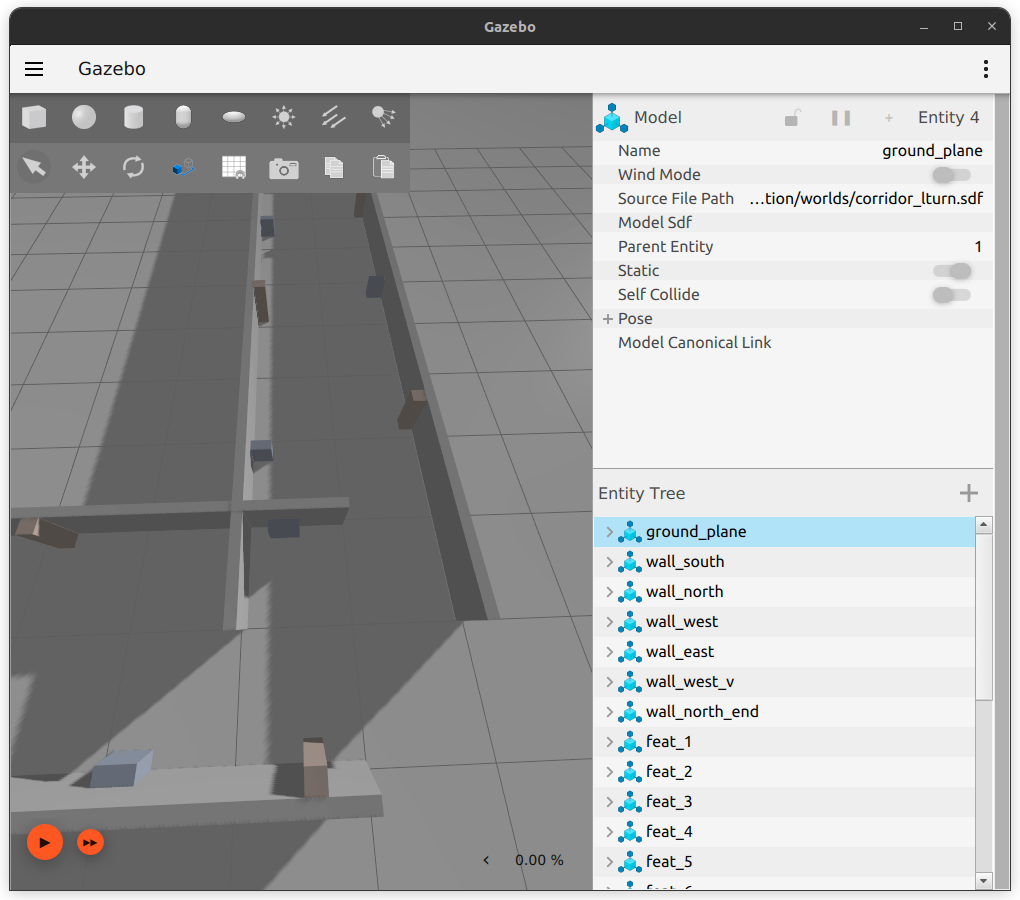
\includegraphics[width=0.7\textwidth]{01_lturn_broken_walls_gazebo.png}
  \caption{L-turn corridor before fix: Gazebo view showing the broken wall
    geometry. The outer corner has a gap (wall ends don't meet) and the inner
    wall segment protrudes into the vertical corridor. Entity tree still shows
    old wall names (\texttt{wall\_south}, \texttt{wall\_east}, etc.).}
\end{figure}

\note{The T-junction (\texttt{corridor\_tjunction.sdf}) was also audited and found
correct --- its north wall is properly split into left (x=$-$7.5 to $-$1) and
right (x=+1 to +7.5) segments with branch walls starting at the gap edges.
\texttt{corridor\_doorway.sdf} was also verified correct.}

\subsection*{SLAM Map Generation: Perceptual Aliasing}

\logentry{First Mapping Attempt --- L-Turn}
After fixing the wall geometry, SLAM Toolbox was launched on the L-turn corridor.
The resulting map showed severe \textbf{warping and folding} --- the classic
signature of \textbf{perceptual aliasing}. The two legs of the L-turn have
identical 2m width and similar feature patterns. SLAM Toolbox's correlative
scan matcher ``recognized'' one leg as the other and incorrectly snapped the
pose, causing the map to fold onto itself.

\issue{In Gazebo, perceptual aliasing is \emph{worse} than real hardware:}
Simulated LiDAR returns mathematically identical profiles in similar corridor
segments with zero noise, sensor droop, or surface irregularity to differentiate
them. Real walls have slight imperfections that provide disambiguating texture.

\logentry{Root Cause Analysis}
The original SLAM Toolbox parameters were configured aggressively for loop closing:
\begin{itemize}
  \item \texttt{do\_loop\_closing: true} --- allowed false loop closures between
    similar-looking corridor segments
  \item \texttt{loop\_search\_maximum\_distance: 8.0} --- in a 2m corridor, this
    let SLAM match scans from one leg against the other leg
  \item \texttt{do\_relocalization: true} --- compounded false matching
  \item \texttt{ceres\_loss\_function: None} --- no protection against outlier
    matches pulling the pose
  \item \texttt{loop\_search\_space\_dimension: 10.0} --- massive search window
  \item \texttt{correlation\_search\_space\_dimension: 1.0} --- too wide for
    near-perfect Gazebo odometry
\end{itemize}

\logentry{Fix: SLAM Toolbox Parameter Tuning for Gazebo Corridors}
\textbf{Key insight:} Gazebo odometry (from \texttt{ackermann\_steering\_controller}
$\to$ EKF) is near-perfect. SLAM should only \emph{refine} the pose locally,
never override it with a distant match.

\begin{center}
\begin{tabular}{lll}
\textbf{Parameter} & \textbf{Before} & \textbf{After} \\
\hline
\texttt{ceres\_loss\_function} & None & \textbf{HuberLoss} \\
\texttt{do\_loop\_closing} & true & \textbf{false} \\
\texttt{do\_relocalization} & true & \textbf{false} \\
\texttt{correlation\_search\_space\_dimension} & 1.0 & \textbf{0.5} \\
\texttt{correlation\_search\_space\_resolution} & 0.02 & \textbf{0.01} \\
\texttt{loop\_search\_space\_dimension} & 10.0 & \textbf{4.0} \\
\texttt{loop\_search\_maximum\_distance} & 8.0 & \textbf{3.0} \\
\texttt{coarse\_search\_angle\_offset} & 0.9 & \textbf{0.5} \\
\texttt{use\_response\_expansion} & true & \textbf{false} \\
\texttt{minimum\_angle\_penalty} & 0.7 & \textbf{0.9} \\
\texttt{minimum\_distance\_penalty} & 0.3 & \textbf{0.5} \\
\texttt{link\_scan\_maximum\_distance} & 3.0 & \textbf{1.5} \\
\texttt{loop\_match\_minimum\_response\_coarse} & 0.25 & \textbf{0.35} \\
\texttt{loop\_match\_minimum\_response\_fine} & 0.35 & \textbf{0.45} \\
\texttt{loop\_match\_minimum\_chain\_size} & 6 & \textbf{10} \\
\texttt{correlation\_search\_space\_smear\_deviation} & 0.1 & \textbf{0.05} \\
\end{tabular}
\end{center}

\textbf{Rationale per parameter:}
\begin{itemize}
  \item \textbf{HuberLoss}: Robust cost function that down-weights outlier scan
    matches, preventing a single bad match from pulling the entire pose estimate.
  \item \textbf{do\_loop\_closing: false}: Prevents the scan matcher from
    ``recognizing'' one corridor leg as another. Safe in Gazebo because odom
    drift is negligible over 10--20m mapping runs.
  \item \textbf{Tighter search spaces}: \texttt{correlation\_search\_space\_dimension:
    0.5} and \texttt{resolution: 0.01} mean the scan matcher only looks within
    $\pm$0.25m of the odom-predicted pose, with finer resolution. This trusts
    Gazebo's near-perfect odometry.
  \item \textbf{Higher penalties}: \texttt{minimum\_angle\_penalty: 0.9} and
    \texttt{minimum\_distance\_penalty: 0.5} make the matcher more conservative
    about accepting distant or rotated matches.
  \item \textbf{use\_response\_expansion: false}: Prevents automatic widening of
    the search window when the initial match is weak --- in a repetitive corridor,
    expanding the search is exactly what causes aliasing.
\end{itemize}

\begin{figure}[h]
  \centering
  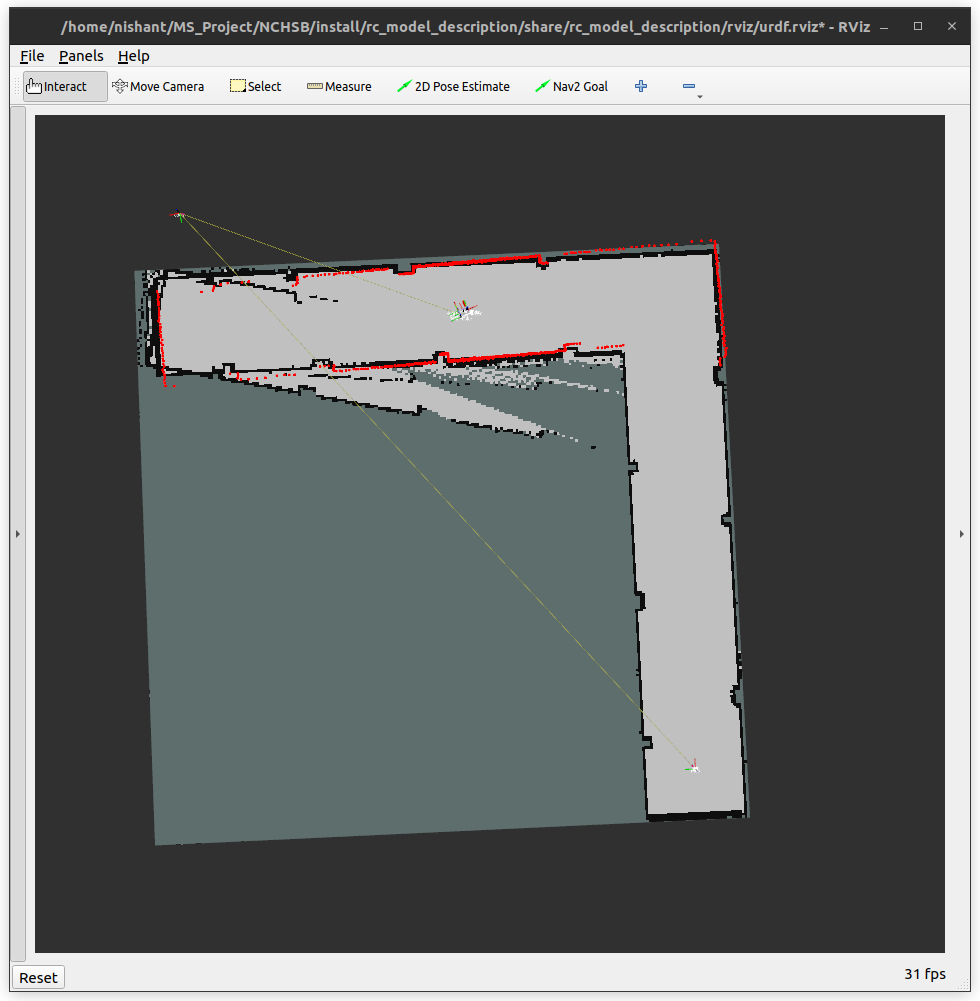
\includegraphics[width=0.7\textwidth]{02_lturn_perceptual_aliasing_warped_map.png}
  \caption{L-turn corridor: Perceptual aliasing with original SLAM params.
    The map is warped and folded --- the two corridor legs have identical LiDAR
    profiles, causing the scan matcher to incorrectly ``recognize'' one leg as
    the other and snap the pose. Classic loop closure failure in repetitive
    environments.}
\end{figure}

\logentry{Result After Tuning}
After applying the tuned parameters, the L-turn map generated correctly:
clean horizontal leg, sharp 90-degree corner, clean vertical leg, with wall
features visible as small indentations in the occupancy grid. No warping,
folding, or ghosting.

\begin{figure}[h]
  \centering
  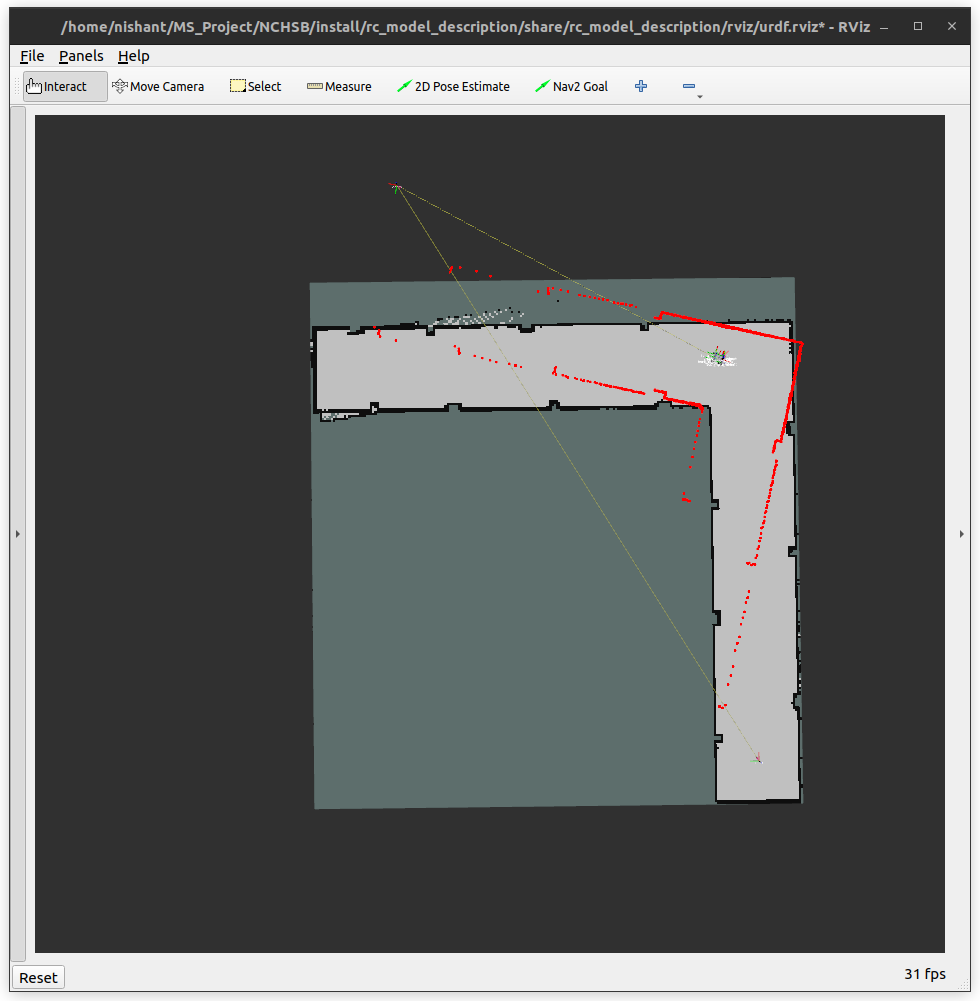
\includegraphics[width=0.48\textwidth]{03_lturn_scan_rotates_with_bot.png}
  \hfill
  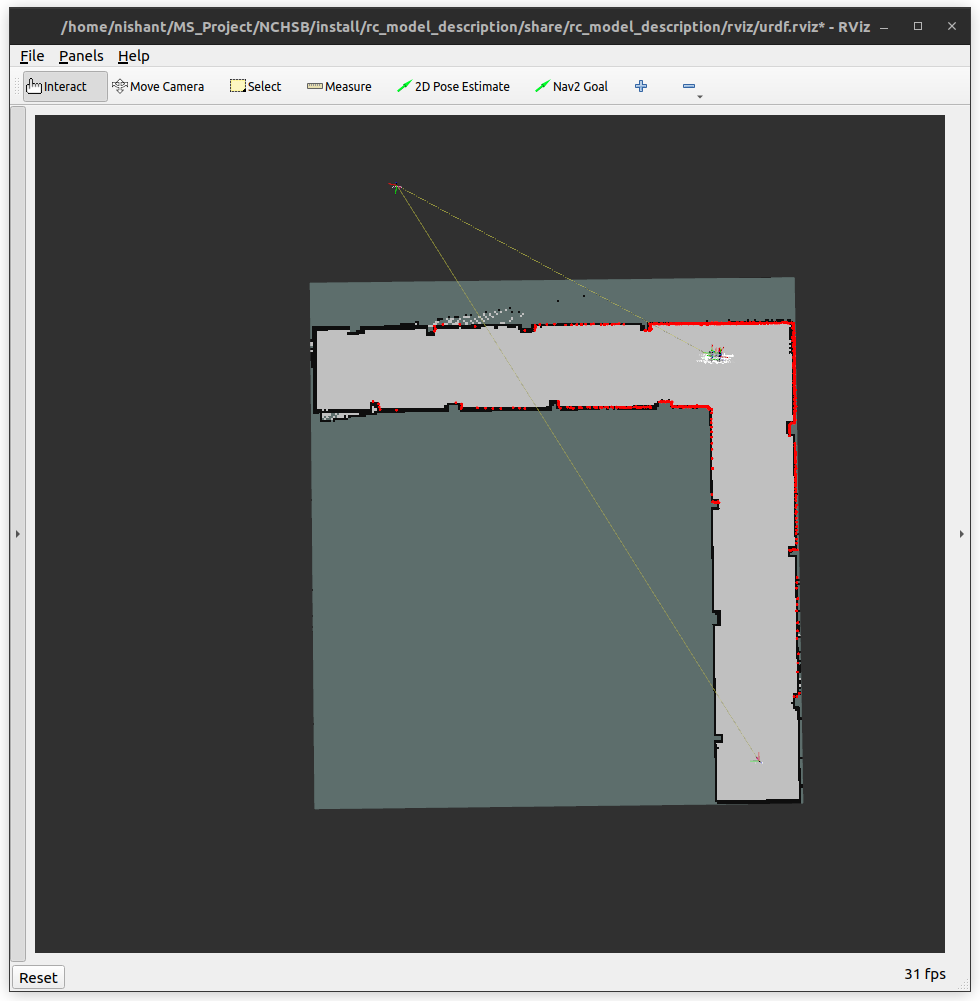
\includegraphics[width=0.48\textwidth]{04_lturn_scan_aligned_correct.png}
  \caption{L-turn corridor after SLAM param tuning. \textbf{Left}: LiDAR scan
    (red dots) rotates with the robot during a turn --- this is \emph{normal}
    (scan is in \texttt{lidar\_link} frame). \textbf{Right}: When stationary,
    the red dots align precisely with the black walls in the occupancy grid,
    confirming correct TF chain and SLAM alignment.}
\end{figure}

\note{The LiDAR scan (red dots in RViz) rotating with the robot is
\textbf{normal and expected behavior}. The scan is published in the
\texttt{lidar\_link} frame (attached to the robot). RViz transforms it via
\texttt{lidar\_link $\to$ base\_link $\to$ odom $\to$ map}. The diagnostic is
whether the red dots \emph{align with the black walls} in the occupancy grid.
Alignment = correct. Persistent offset = TF or SLAM error.}

\note{For the closed-loop corridor (\texttt{corridor\_loop.sdf}), loop closure
IS needed because the robot physically revisits the same location. A separate
SLAM params file with \texttt{do\_loop\_closing: true} should be used for that
world only.}

\subsection*{Mapping Tips for Gazebo Corridors}

Based on the mapping experience, the following practices produce clean maps:
\begin{enumerate}
  \item \textbf{Drive slowly} ($\sim$0.2 m/s). More scan overlap = less chance of
    a bad match. At 0.5 m/s with 25 Hz LiDAR, inter-scan motion is 2cm --- good.
    At 1.0 m/s, it's 4cm --- still OK but more risk in featureless segments.
  \item \textbf{Use \texttt{slam\_params\_file}, NOT \texttt{params\_file}} when
    launching SLAM Toolbox. The launch file \texttt{online\_async\_launch.py}
    expects the argument \texttt{slam\_params\_file} to load custom configuration.
    Using \texttt{params\_file} silently ignores the custom config and uses
    defaults (including \texttt{base\_frame: base\_footprint}, which doesn't exist
    in our robot's TF tree).
  \item \textbf{Map save command:}
\begin{lstlisting}
mkdir -p ~/MS_Project/NCHSB/maps
ros2 run nav2_map_server map_saver_cli \
    -f maps/corridor_<name> \
    --ros-args -p use_sim_time:=true
\end{lstlisting}
    This produces \texttt{corridor\_<name>.pgm} + \texttt{corridor\_<name>.yaml}.
\end{enumerate}

\subsection*{Correct Spawn Points for All 6 Corridor Worlds}

Several corridors have different extents. Using \texttt{spawn\_x:=-9.0} for all
worlds caused the robot to spawn outside shorter corridors. Correct spawn points:

\begin{center}
\begin{tabular}{llll}
\textbf{World SDF} & \textbf{spawn\_x} & \textbf{spawn\_y} & \textbf{Corridor Extent} \\
\hline
\texttt{corridor\_straight} & $-9.0$ & $0.0$ & x: $-$10 to +10 \\
\texttt{corridor\_lturn} & $-9.0$ & $0.0$ & horiz: x $-$10 to 0 \\
\texttt{corridor\_tjunction} & $-6.0$ & $0.0$ & x: $-$7.5 to +7.5 \\
\texttt{corridor\_narrow} & $-6.5$ & $0.0$ & x: $-$7.5 to +7.5 \\
\texttt{corridor\_doorway} & $-6.5$ & $0.0$ & x: $-$7.5 to +7.5 \\
\texttt{corridor\_loop} & $-8.0$ & $-4.0$ & outer 20$\times$10m \\
\end{tabular}
\end{center}

\subsection*{Previous Session TF \& SLAM Debugging (2026-03-05/06) --- Summary}

The following critical issues were identified and resolved during the initial
SLAM map generation sessions. They are recorded here for future reference and
to assist with the paper's system description.

\subsubsection*{Bug: EKF Namespace Mismatch}
\begin{itemize}
  \item \issue{The \texttt{robot\_localization} EKF config file used namespace
    \texttt{ekf\_imu\_odom:} but the default node name is \texttt{ekf\_filter\_node}.
    All parameters were silently ignored.}
  \item \fix{Changed namespace in \texttt{ekf\_imu\_odom.yaml} from
    \texttt{ekf\_imu\_odom:} to \texttt{ekf\_filter\_node:}.}
  \item \fix{Removed \texttt{imu0} input (no IMU sensor defined in URDF).}
\end{itemize}

\subsubsection*{Bug: TRANSIENT\_LOCAL QoS on /tf Causing Time Jumps}
\begin{itemize}
  \item \issue{The \texttt{gazebo\_control.xacro} contained a remapping:
    \texttt{ackermann\_steering\_controller/tf\_odometry:=tf}. This caused the
    ackermann controller to publish \texttt{odom $\to$ base\_link} TF on
    \texttt{/tf} with \texttt{TRANSIENT\_LOCAL} QoS durability. When Gazebo
    restarted, old high-timestamped messages from previous runs were replayed
    to late-joining subscribers (RViz, SLAM Toolbox), causing ``Detected jump
    back in time. Clearing TF buffer.'' errors.}
  \item \fix{Removed the \texttt{tf\_odometry} remapping from
    \texttt{gazebo\_control.xacro}. Set \texttt{enable\_odom\_tf: false} in
    \texttt{controllers.yaml}. The EKF is now the sole publisher of
    \texttt{odom $\to$ base\_link} TF on \texttt{/tf} with \texttt{VOLATILE}
    QoS (default for \texttt{robot\_localization}).}
\end{itemize}

\subsubsection*{Bug: EKF predict\_to\_current\_time Causing TF Timestamp Issues}
\begin{itemize}
  \item \issue{Setting \texttt{predict\_to\_current\_time: true} in the EKF
    caused TF timestamps to jump backward when real measurements (odom) arrived,
    because the EKF would extrapolate to wall-clock time, then snap back to
    measurement time.}
  \item \fix{Set \texttt{predict\_to\_current\_time: false}. Added
    \texttt{transform\_time\_offset: 0.05} to ensure EKF TF timestamps are
    slightly ahead of scan timestamps, preventing ``extrapolation into the
    future'' errors in SLAM Toolbox.}
\end{itemize}

\subsubsection*{Bug: SLAM Toolbox Launch Argument Name}
\begin{itemize}
  \item \issue{The \texttt{slam\_toolbox} launch file
    \texttt{online\_async\_launch.py} expects the parameter
    \texttt{slam\_params\_file} to load custom configuration, but we were passing
    \texttt{params\_file}. This meant the custom config (which sets
    \texttt{base\_frame: base\_link}) was \emph{never loaded}. SLAM Toolbox used
    its default \texttt{base\_frame: base\_footprint}, which does not exist in
    our TF tree, causing continuous ``Failed to compute odom pose'' errors.}
  \item \fix{Changed the launch argument from \texttt{params\_file} to
    \texttt{slam\_params\_file}.}
\end{itemize}

\subsubsection*{Bug: Teleop Not Moving Robot}
\begin{itemize}
  \item \issue{\texttt{teleop\_twist\_keyboard} publishes
    \texttt{geometry\_msgs/msg/Twist} to \texttt{/cmd\_vel}, but the
    \texttt{ackermann\_steering\_controller} was configured with
    \texttt{use\_stamped\_vel: true}, expecting
    \texttt{geometry\_msgs/msg/TwistStamped} on
    \texttt{/ackermann\_steering\_controller/reference}.}
  \item \fix{Set \texttt{use\_stamped\_vel: false} in \texttt{controllers.yaml}.
    Teleop must publish to
    \texttt{/ackermann\_steering\_controller/reference\_unstamped}.}
\end{itemize}

\subsubsection*{Bug: EKF Not Starting with Gazebo}
\begin{itemize}
  \item \issue{Launching the EKF node separately (after Gazebo) caused race
    conditions --- the EKF sometimes started before \texttt{/odom} was available,
    or SLAM started before the EKF published \texttt{odom $\to$ base\_link} TF.}
  \item \fix{Added the EKF node directly to
    \texttt{fortress\_bringup.launch.py} so it starts alongside Gazebo and
    the robot, eliminating launch-order dependencies.}
\end{itemize}

\subsubsection*{Configuration: Miniconda Python Interference}
\begin{itemize}
  \item \issue{Diagnostic Python scripts failed with
    \texttt{ModuleNotFoundError: No module named 'rclpy.\_rclpy\_pybind11'}
    when Miniconda's Python 3.13 was active.}
  \item \fix{Use \texttt{/usr/bin/python3} explicitly instead of \texttt{python3}
    to ensure the system's Python 3.10 (compatible with ROS 2 Humble) is used.}
\end{itemize}

\subsection*{Files Modified in This Session}

\begin{itemize}
  \item \texttt{src/rc\_model\_description/worlds/corridor\_lturn.sdf} --- Complete
    rewrite of wall geometry (6 walls forming correct L-boundary + 14 features).
  \item \texttt{src/rc\_model\_description/config/mapper\_params\_online\_async.yaml}
    --- SLAM Toolbox parameter tuning (16 parameters changed to prevent
    perceptual aliasing).
\end{itemize}

\subsection*{T-Junction: Cabinet Feature Orientation \& Scan Matching Iteration}

\begin{figure}[h]
  \centering
  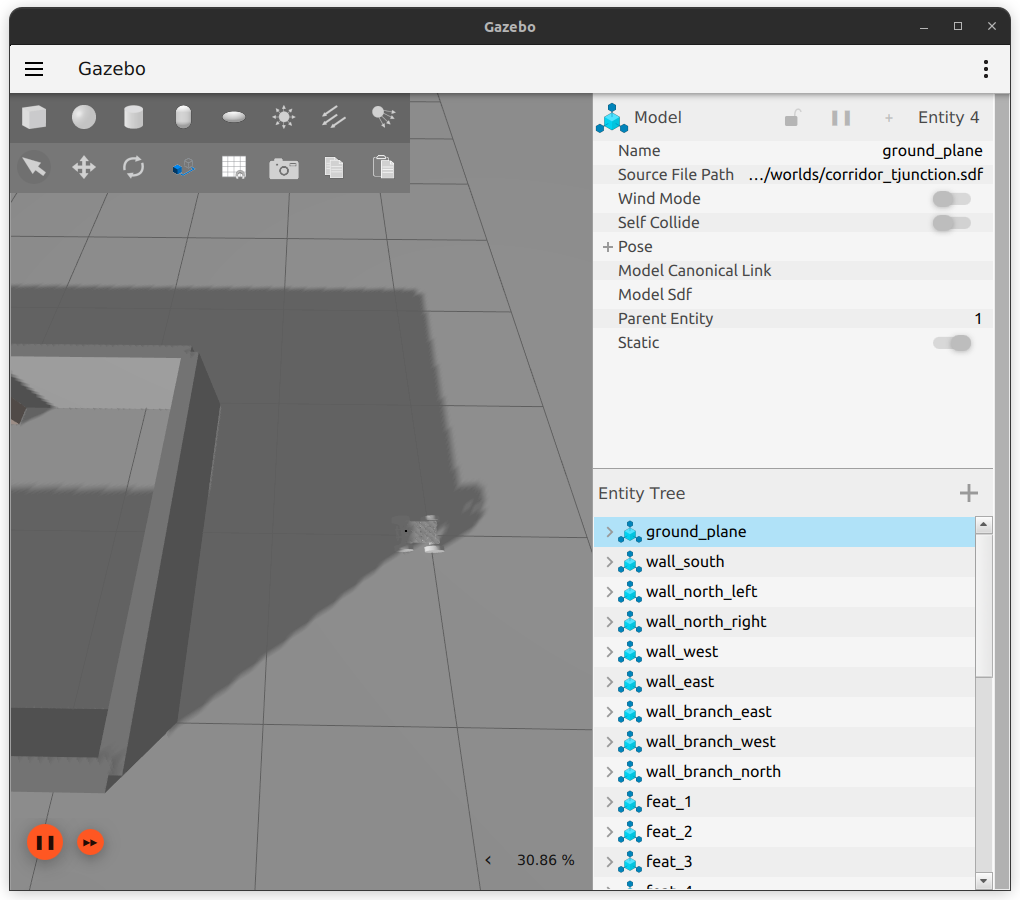
\includegraphics[width=0.7\textwidth]{05_tjunction_bot_outside_corridor.png}
  \caption{T-junction: Robot spawned outside corridor walls when using
    \texttt{spawn\_x:=-9.0}. The west wall is at x=$-$7.5, so spawn must be
    inside (e.g.\ \texttt{spawn\_x:=-6.0}).}
\end{figure}

\logentry{T-Junction Branch Wall Features}
The T-junction branch corridor (vertical segment) had cabinet features
(\texttt{feat\_12}, \texttt{feat\_14}, \texttt{feat\_15}, \texttt{feat\_17})
with swapped dimensions: \texttt{0.3 x 0.12} instead of \texttt{0.12 x 0.3}.
\begin{itemize}
  \item \issue{For walls running along Y (branch east/west walls), cabinets
    should protrude 0.12\,m in X and span 0.3\,m along the corridor in Y.
    The wrong orientation had them protruding 0.3\,m (15\% of corridor width!)
    into the 2\,m branch, with only 0.12\,m visible along the corridor.}
  \item \fix{Changed all four branch cabinet features from \texttt{<size>0.3 0.12
    0.25</size>} to \texttt{<size>0.12 0.3 0.25</size>}. Adjusted X pose
    from 0.875 to 0.89 (and $-0.875$ to $-0.89$) for proper protrusion.}
\end{itemize}

\begin{figure}[h]
  \centering
  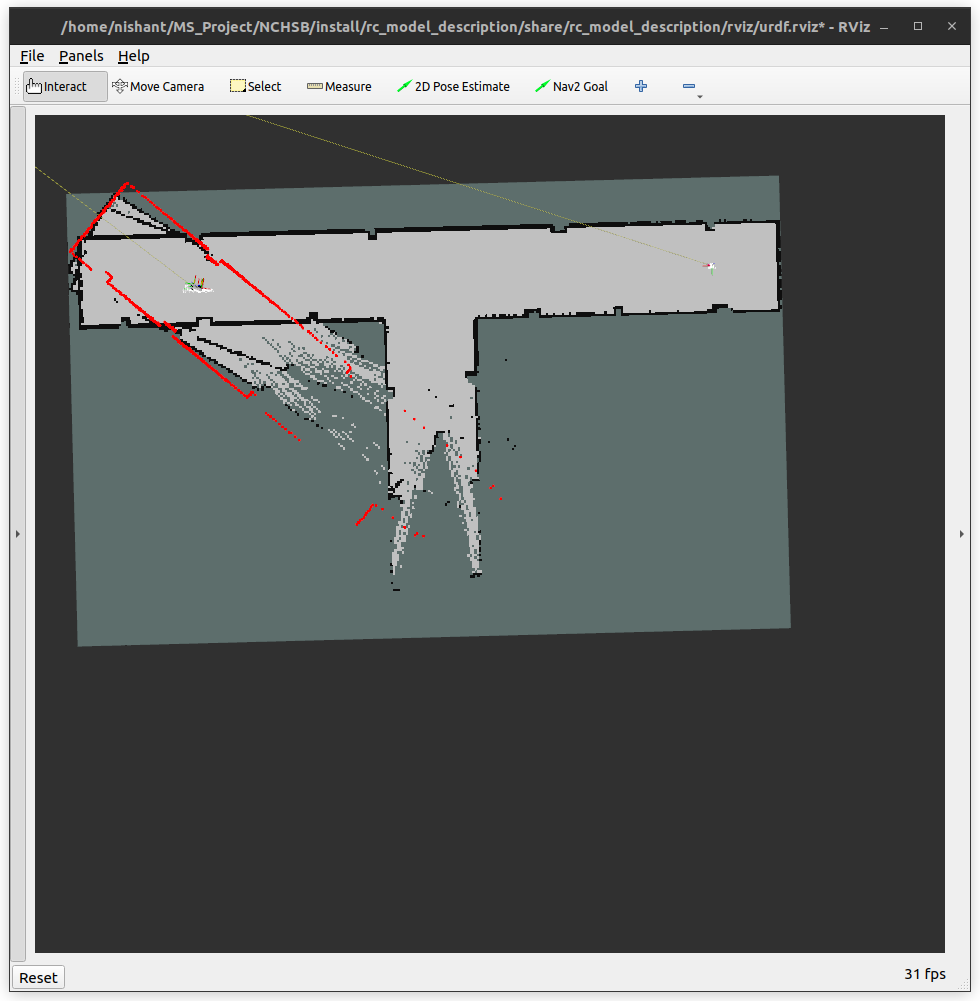
\includegraphics[width=0.48\textwidth]{06_tjunction_branch_ghosting_scan_matching_on.png}
  \hfill
  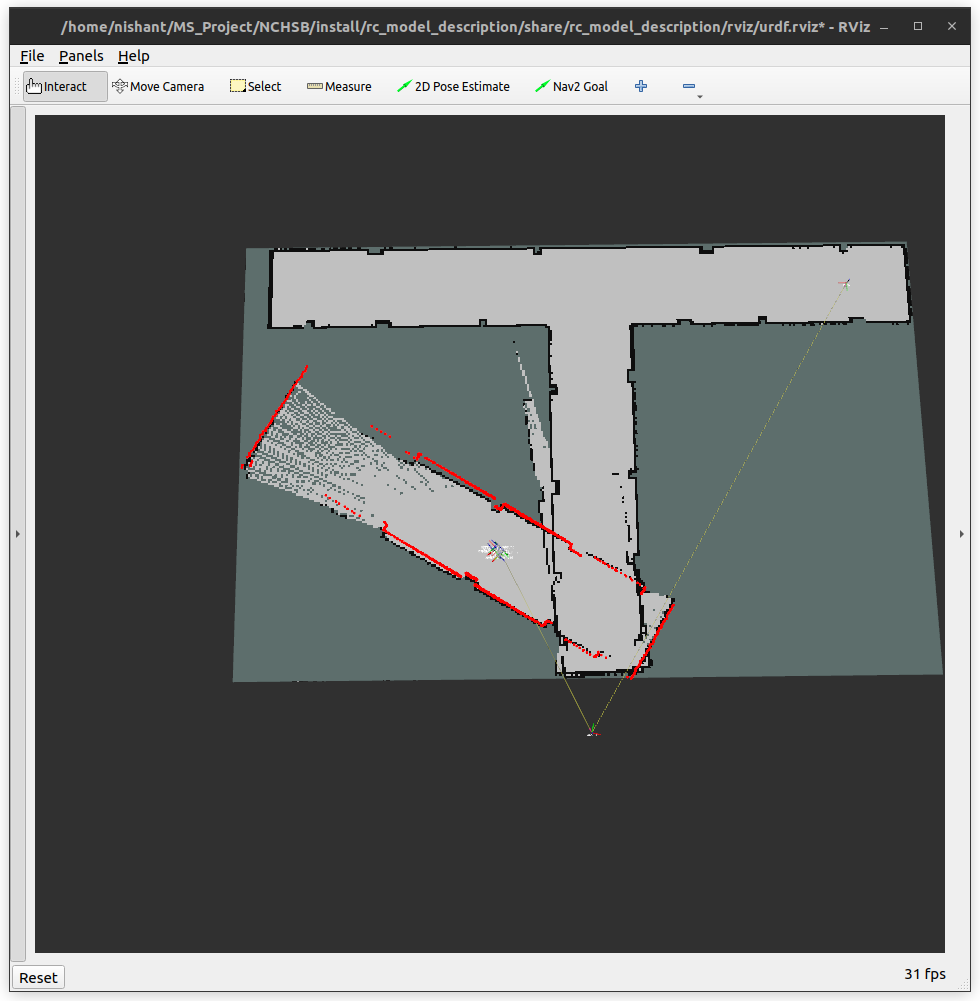
\includegraphics[width=0.48\textwidth]{07_tjunction_angular_drift_scan_matching_on.png}
  \caption{T-junction: Scan matching ON with wide search window.
    \textbf{Left}: Branch corridor shows ghosting/blurring with overlapping
    wall traces. \textbf{Right}: Branch mapped at $\sim$45$^\circ$ instead of
    90$^\circ$ --- the scan matcher accumulated angular drift at the junction.}
\end{figure}

\logentry{Attempt 1: Disable Scan Matching Entirely}
To eliminate perceptual aliasing at junctions, \texttt{use\_scan\_matching} was
set to \texttt{false}. The hypothesis: Gazebo odom is near-perfect, so SLAM
should trust it completely.
\begin{itemize}
  \item \issue{Result was \textbf{worse}. The map showed severe ``fanning'' ---
    scans radiating outward in multiple directions. Straight corridor mapped
    fine; as soon as the robot turned or reversed, scans misaligned. The red
    LiDAR points ``moved a bit back'' (shifted) when coming back along the
    corridor.}
  \item \fix{Root cause: Ackermann odometry has small yaw drift that
    accumulates during turns and reverse. Without scan matching to correct it,
    each scan is placed at a slightly wrong angle; the drift compounds and
    produces the fanning pattern. Scan matching is \emph{needed} to fix odom
    drift; the problem was that it was making corrections that were too large.}
\end{itemize}

\begin{figure}[h]
  \centering
  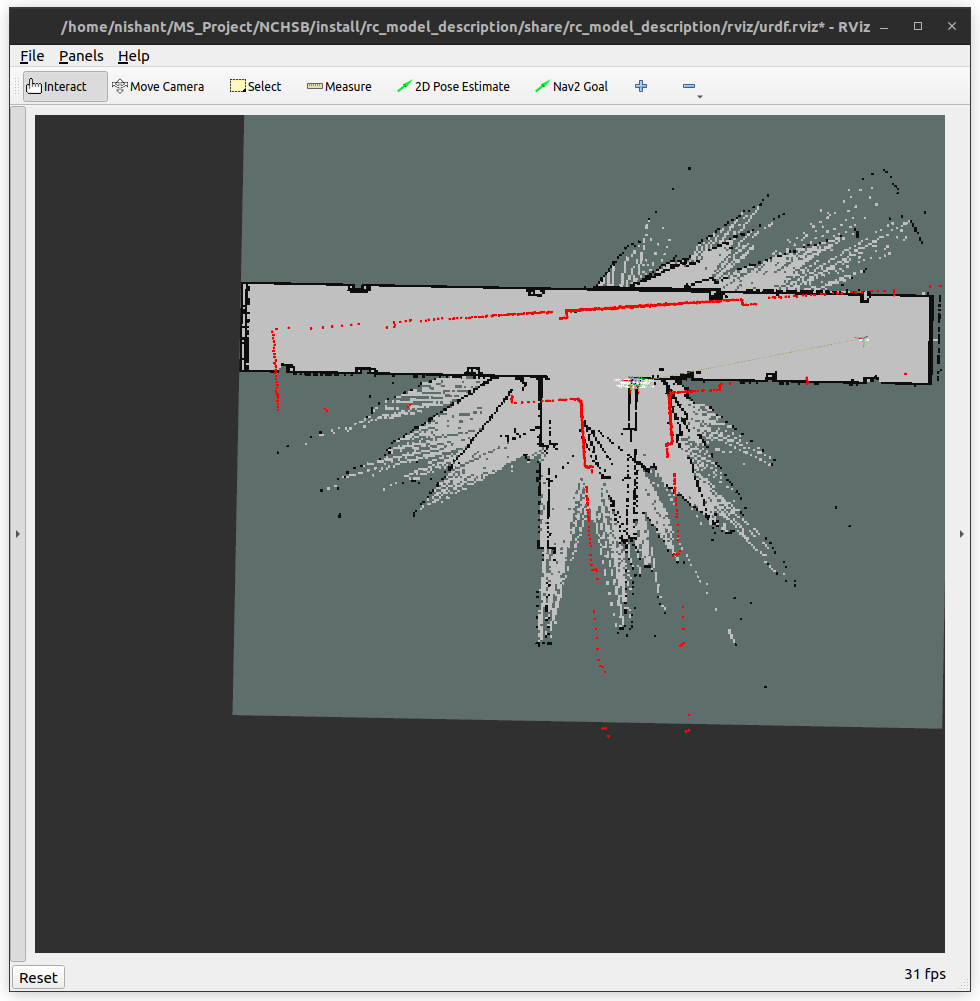
\includegraphics[width=0.7\textwidth]{08_tjunction_fanning_scan_matching_off.png}
  \caption{T-junction: Scan matching OFF (\texttt{use\_scan\_matching: false}).
    Severe ``fanning'' pattern --- each scan placed at a slightly different
    angle due to accumulated odom yaw drift. Main corridor mapped fine;
    the fanning appeared at the junction where the robot turned.}
\end{figure}

\logentry{Attempt 2: Tightly Constrained Scan Matching}
Re-enabled scan matching but constrained it so it can only make \emph{small}
corrections (fixing drift) and cannot make large jumps (which cause aliasing).
\begin{center}
\begin{tabular}{lll}
\textbf{Parameter} & \textbf{Previous} & \textbf{Final} \\
\hline
\texttt{use\_scan\_matching} & false & \textbf{true} \\
\texttt{minimum\_travel\_distance} & 0.50 & \textbf{0.15} \\
\texttt{minimum\_travel\_heading} & 0.35 & \textbf{0.10} \\
\texttt{correlation\_search\_space\_dimension} & 0.5 & \textbf{0.3} \\
\texttt{coarse\_search\_angle\_offset} & 0.5 & \textbf{0.15} \\
\texttt{coarse\_angle\_resolution} & 0.0349 & \textbf{0.01} \\
\texttt{angle\_variance\_penalty} & 0.5 & \textbf{1.0} \\
\texttt{correlation\_search\_space\_smear\_deviation} & 0.05 & \textbf{0.03} \\
\end{tabular}
\end{center}
\textbf{Rationale:}
\begin{itemize}
  \item \textbf{Frequent scans} (0.15\,m, 0.10\,rad): Smaller pose change between
    scans $\Rightarrow$ scan matcher has less room to go wrong. Critical at
    junction turns where angular change is rapid.
  \item \textbf{Tight search} (0.3\,m, 0.15\,rad $\approx$ 8.5$^\circ$): Matcher
    can only shift pose $\pm$15\,cm and rotate $\pm$8.5$^\circ$ max. Fixes
    sub-centimeter odom drift without being able to ``jump'' to an aliased
    location.
  \item \textbf{Higher angle\_variance\_penalty}: Strongly penalize angular
    deviations so the matcher prefers small corrections.
\end{itemize}

\fix{Result: This configuration worked. The T-junction maps cleanly with
correct 90-degree branch alignment, no fanning, and no perceptual aliasing.
Straight corridor, L-turn, and T-junction all map correctly with the same
params.}

\note{Teleop speed 0.5\,m/s is fine for mapping. The earlier ``drive slowly''
advice applied when scan matching was active with wider search; with tight
constraints, speed matters less.}

\subsection*{Narrow Corridor: Symmetric Features \& Missing Narrow Section Features}

\begin{figure}[h]
  \centering
  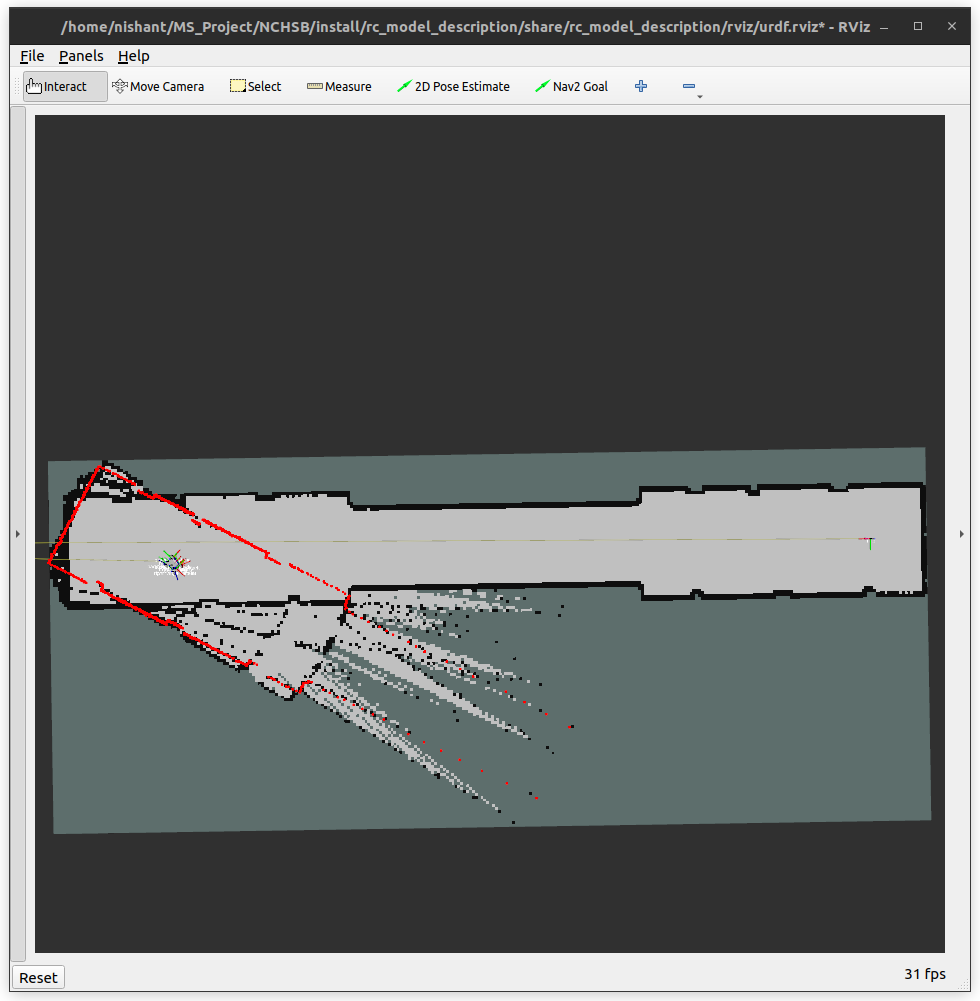
\includegraphics[width=0.7\textwidth]{09_narrow_fanning_symmetric_features.png}
  \caption{Narrow corridor: Fanning/ghosting below the main corridor caused by
    the scan matcher confusing the left and right sections (identical feature
    patterns) and the featureless narrow center section.}
\end{figure}

\logentry{Root Cause}
The narrow corridor (\texttt{corridor\_narrow.sdf}) had two compounding issues:
\begin{enumerate}
  \item \issue{Left and right sections had identical (mirror-image) feature
    patterns: same feature types in the same order with the same 1.5\,m gaps.
    To the LiDAR, the left 2\,m-wide section looked exactly like the right
    2\,m-wide section.}
  \item \issue{The narrow center section (x=$-$2.5 to $+$2.5, 1.5\,m wide)
    had \textbf{zero features} --- 5\,m of featureless corridor. The width
    change at the transition walls was the only distinguishing element.}
\end{enumerate}

\logentry{Fix}
Rewrote \texttt{corridor\_narrow.sdf} with asymmetric features:
\begin{itemize}
  \item \textbf{Left section}: 2 south (pillar, large-pillar) + 2 north
    (cabinet, pillar). Gaps: 2.6\,m, 2.5\,m.
  \item \textbf{Narrow section}: Added 3 features (2 south + 1 north) with
    smaller protrusions (0.25$\times$0.12 cabinets) to fit the tighter 1.5\,m
    width. Features positioned asymmetrically.
  \item \textbf{Right section}: 3 south (cabinet, pillar, cabinet) + 2 north
    (large-pillar, cabinet). Gaps: 1.2\,m, 2.0\,m --- deliberately different
    from the left section.
  \item Introduced a third feature size class (\textbf{large-pillar}:
    0.20$\times$0.20) used only in the left and right sections at different
    positions (south in left, north in right) to break symmetry.
\end{itemize}

\subsection*{Narrow Corridor: U-Turn Scan Misalignment (Expected Behavior)}

\begin{figure}[h]
  \centering
  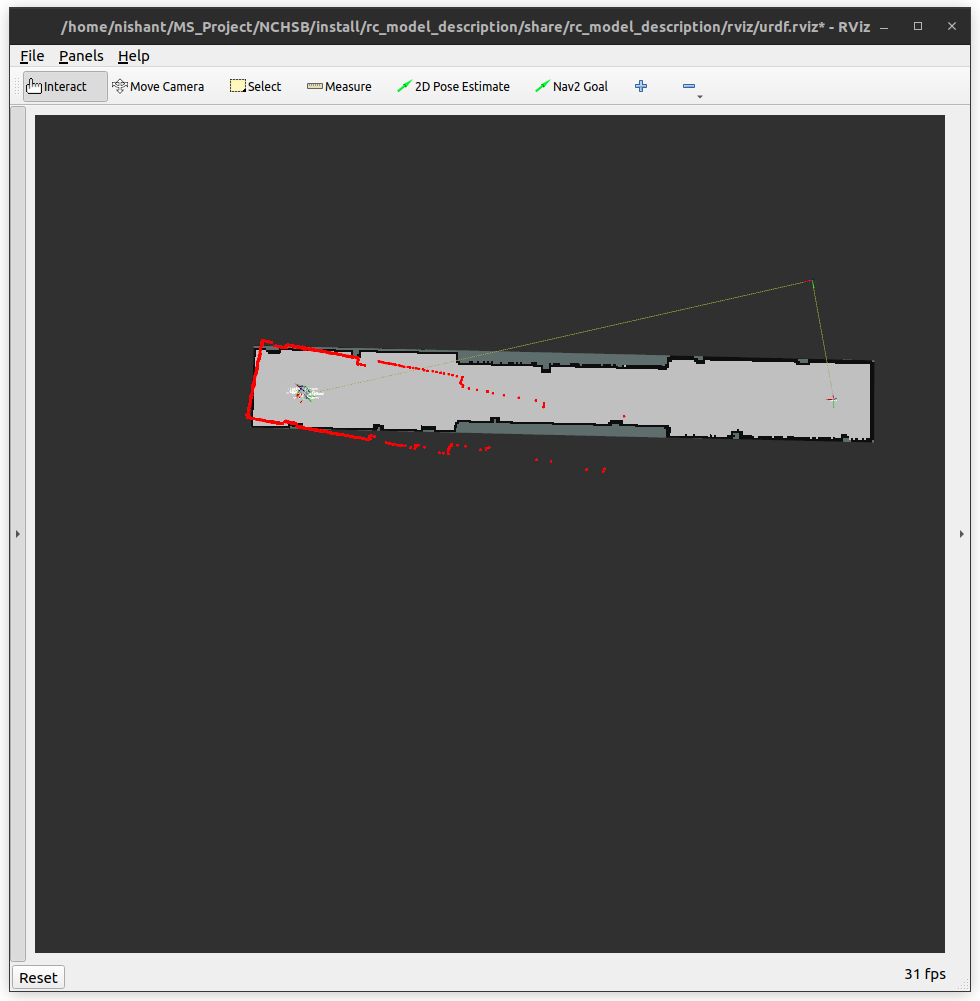
\includegraphics[width=0.48\textwidth]{10_narrow_uturn_mid_scan_misalign.png}
  \hfill
  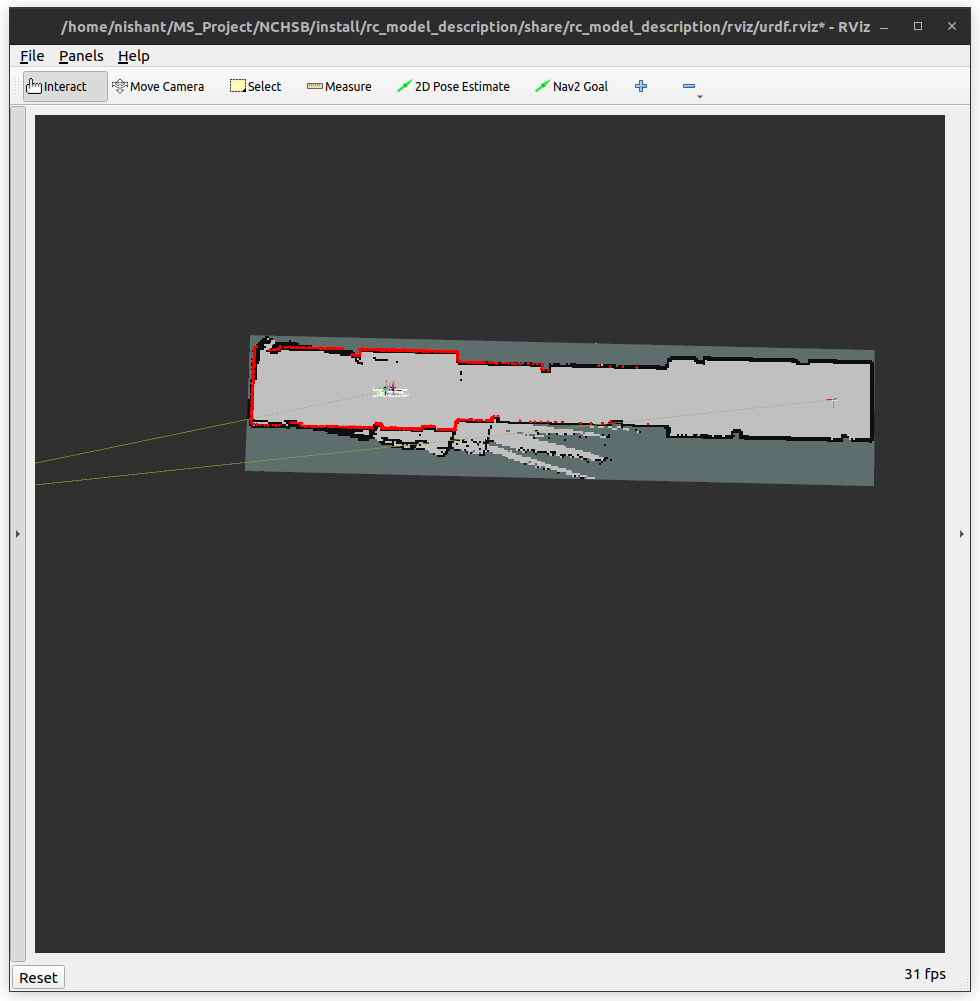
\includegraphics[width=0.48\textwidth]{11_narrow_uturn_complete_overlap_noise.png}
  \caption{\textbf{Left}: Mid-U-turn at the corridor end --- the red LiDAR dots
    are misaligned from the black walls. The robot is rotating in place, and
    during the turn the scan matcher receives a rapidly changing scan profile
    (walls are at different angles each frame) which it cannot reliably match.
    \textbf{Right}: After completing the full 180$^\circ$ U-turn, the scan
    realigns with the walls and the corridor maps correctly again. The grey
    ``noise'' around the turn point is the accumulated scans from the rotation,
    which is cosmetic.}
\end{figure}

\logentry{Analysis}
This is \textbf{expected behavior}, not a bug:
\begin{itemize}
  \item During a U-turn in a narrow corridor, the robot rotates $\sim$180$^\circ$
    in place. Each scan during the rotation sees the corridor walls at a
    different angle. The scan matcher's correlation search window
    (\texttt{coarse\_search\_angle\_offset: 0.15\,rad $\approx$ 8.5$^\circ$})
    is much smaller than the total rotation, so it \emph{cannot} match
    consecutive scans during a fast turn. This produces the mid-turn
    misalignment visible in image~1.
  \item Once the turn completes and the robot faces back down the corridor,
    the scan profile returns to ``two parallel walls'' and the matcher
    re-locks correctly. The walls realign (image~2).
  \item The grey smear around the turn point is cosmetic --- the occupancy
    grid accumulated uncertain readings during the fast rotation. For
    Nav2 navigation, the turn point is not part of the navigable corridor
    center, so this does not affect path planning.
  \item \textbf{Mitigation for cleaner maps}: Turn slowly. At 0.5\,m/s with
    the Ackermann turning radius, a U-turn at the corridor end takes several
    seconds. With \texttt{minimum\_travel\_heading: 0.10\,rad}, the mapper
    processes a scan every $\sim$6$^\circ$ of rotation, giving the matcher
    sufficient overlap between consecutive scans.
  \item \fix{Verified: slow speed during U-turns produces cleaner maps with
    less grey smear at the turn point.}
\end{itemize}

\note{This behavior will not affect experiments: the robot never U-turns during
trials --- it drives from start to goal in one direction. Maps only need clean
walls along the navigable corridor, not perfect coverage at the dead ends.}

\subsection*{Doorway Corridor: Insufficient \& Repetitive Features}

\logentry{Pre-mapping Audit}
Before mapping \texttt{corridor\_doorway.sdf}, audited features for uniqueness.

\issue{Multiple problems found:}
\begin{enumerate}
  \item Only 10 features for a 15\,m corridor with two alcoves --- too few.
  \item The 7.5\,m east segment of the north wall (x=$-$2.75 to +2.0) had
    only 2 features at x=6.0 and x=7.0, leaving the first 6\,m featureless.
  \item West and east segment patterns were near-mirrors: pillar-cabinet-pillar
    vs.\ cabinet-pillar-pillar with similar 1.5--2.0\,m gaps.
  \item Alcove interiors (back walls, side walls) had zero features.
\end{enumerate}

\logentry{Fix}
Rewrote features for \texttt{corridor\_doorway.sdf} (10 $\to$ 14 features):
\begin{itemize}
  \item \textbf{South wall west}: large-pillar($-$6.8), cabinet($-$4.5).
    Gap: 2.3\,m.
  \item \textbf{North wall west}: pillar($-$6.2), large-pillar($-$3.8),
    cabinet($-$1.2), pillar(0.8). Gaps: 2.4, 2.6, 2.0\,m --- all distinct.
  \item \textbf{Alcove 1 interior}: pillar on west side wall (y=1.9),
    cabinet on back wall (x=$-$2.0).
  \item \textbf{South wall east}: pillar(1.3), cabinet(3.6),
    large-pillar(6.0). Gaps: 2.3, 2.4\,m.
  \item \textbf{Alcove 2 interior}: large-pillar on east side wall
    (0.12$\times$0.20, oriented for vertical wall), pillar on back wall.
  \item \textbf{North wall east}: cabinet(6.8).
  \item \textbf{Asymmetry}: South-west uses large-pillar+cabinet, south-east
    uses pillar+cabinet+large-pillar --- different order and different feature
    at each position. North wall has 4 features west vs.\ 1 east (compensated
    by alcove 2 providing landmarks in that region).
\end{itemize}

\subsection*{SLAM Map Generation: Complete}

All 6 corridor maps generated successfully via manual teleop driving and saved
with \texttt{map\_saver\_cli}. Files stored in
\texttt{src/rc\_model\_description/maps/}:

\begin{center}
\begin{tabular}{lll}
\textbf{World} & \textbf{Files} & \textbf{Notes} \\
\hline
\texttt{corridor\_straight} & \texttt{.pgm + .yaml} & Clean, no issues \\
\texttt{corridor\_lturn} & \texttt{.pgm + .yaml} & Clean after wall geometry fix \\
\texttt{corridor\_tjunction} & \texttt{.pgm + .yaml} & Clean with tight scan matching \\
\texttt{corridor\_narrow} & \texttt{.pgm + .yaml} & Clean after asymmetric features \\
\texttt{corridor\_doorway} & \texttt{.pgm + .yaml} & Clean after feature redesign \\
\texttt{corridor\_loop} & \texttt{.pgm + .yaml} & Clean without loop closure \\
\end{tabular}
\end{center}

\note{\texttt{corridor\_loop.sdf} mapped cleanly with \texttt{do\_loop\_closing:
false} --- the same params used for all other corridors. No separate params file
was needed. The Gazebo odometry was accurate enough over the loop that scan
matching alone (without loop closure) produced a correct map.}

\subsection*{Files Modified (T-Junction Session)}

\begin{itemize}
  \item \texttt{corridor\_tjunction.sdf} --- Cabinet features feat\_12, 14, 15,
    17: dimensions 0.3$\times$0.12 $\to$ 0.12$\times$0.3, pose X adjusted.
  \item \texttt{mapper\_params\_online\_async.yaml} --- Scan matching re-enabled
    with tight constraints (8 parameters adjusted).
\end{itemize}

% ============================================================
\section{Phase 5: Core Algorithm Implementations}
% ============================================================

This section documents the three core algorithm components that form the paper's
contributions (in addition to the CBF safety shield, documented earlier).

\subsection*{5.1 Corridor Frame Utility (\texttt{corridor\_frame.cpp})}

\logentry{Design Rationale}
The corridor frame is a \textbf{Frenet--Serret reference frame} defined along
the Nav2 global path. It transforms Cartesian coordinates $(x, y)$ into
corridor-aligned coordinates $(s, d)$ where $s$ is arc-length along the corridor
centreline and $d$ is signed lateral offset (positive = left of centreline).
This is the mathematical foundation for the predictive social costmap layer.

\textbf{Why Frenet?} In a corridor, Cartesian predictions spread risk across the
full width even when a pedestrian is clearly walking along one side. The Frenet
frame aligns the prediction with the corridor geometry, making risk tubes narrow
along the lateral axis and extended along the corridor axis --- exactly matching
how pedestrians actually move.

\logentry{Mathematical Formulation}

\textbf{Path representation:} A polyline of $N$ waypoints
$\{(x_0,y_0), \ldots, (x_{N-1},y_{N-1})\}$ extracted from the Nav2 global plan.
Arc-length is pre-computed:
\[
  L_0 = 0, \quad L_i = L_{i-1} + \|(x_i - x_{i-1}, y_i - y_{i-1})\|_2
\]

\textbf{Cartesian $\to$ Frenet} (\texttt{toFrenet}):
For a query point $(x, y)$, find the closest point on the polyline by projecting
onto each segment $[(x_i, y_i), (x_{i+1}, y_{i+1})]$:
\[
  t_i = \mathrm{clamp}\left(
    \frac{(x - x_i)(x_{i+1} - x_i) + (y - y_i)(y_{i+1} - y_i)}
         {\|(x_{i+1} - x_i, y_{i+1} - y_i)\|_2^2},\; 0,\; 1
  \right)
\]
\[
  s = L_i + t_i \cdot \|(\Delta x, \Delta y)\|_2, \quad
  d = \mathrm{sign}(\Delta x \times (y - y_i)) \cdot \|P_\mathrm{query} - P_\mathrm{proj}\|_2
\]
where the cross product determines the sign (positive = left of path direction).

\textbf{Frenet $\to$ Cartesian} (\texttt{toCartesian}):
Given $(s, d)$, find the segment containing $s$ by binary search on $L_i$.
Interpolate the centreline point, compute the unit normal $\hat{n} = (-t_y, t_x)$
(perpendicular to segment tangent), and offset: $(x, y) = P_\mathrm{centreline}
+ d \cdot \hat{n}$.

\textbf{Velocity transformation} (\texttt{toFrenetState}):
Given Cartesian velocity $(v_x, v_y)$ at position $(x, y)$:
\[
  \dot{s} = v_x \cdot t_x + v_y \cdot t_y, \quad
  \dot{d} = -v_x \cdot t_y + v_y \cdot t_x
\]
where $(\hat{t}_x, \hat{t}_y)$ is the unit tangent of the closest segment.

\logentry{Implementation Details}
\begin{itemize}
  \item \textbf{File}: \texttt{src/corridor\_social\_nav/src/corridor\_frame.cpp}
  \item \textbf{Header}: \texttt{include/corridor\_social\_nav/corridor\_frame.hpp}
  \item \textbf{Classes}: \texttt{CorridorFrame}, \texttt{FrenetPoint} (s, d),
    \texttt{FrenetState} (s, d, $\dot{s}$, $\dot{d}$)
  \item \textbf{Path update}: Called whenever Nav2 publishes a new global plan
    on \texttt{/plan}. Recomputes cumulative arc-length array.
  \item \textbf{Projection}: Linear scan over all segments ($O(N)$). Acceptable
    for corridor paths ($N \sim 50$--$200$ waypoints).
  \item \textbf{Edge cases}: Returns $(0, 0)$ if path has $<2$ waypoints.
    Clamps $s$ to $[0, L_\mathrm{total}]$ in \texttt{toCartesian}.
    Skips zero-length segments.
\end{itemize}

% ------------------------------------------------------------------

\subsection*{5.2 Instantaneous Social Costmap Layer (\texttt{social\_layer.cpp})}

\logentry{Design Rationale}
The baseline social navigation approach. Stamps an isotropic Gaussian cost
around each tracked person's \emph{current} position. No prediction, no
velocity information used. This serves as the ``MPPI+Social'' controller
in the paper's comparison table.

\logentry{Mathematical Formulation}
For each person $k$ at position $(p_x^k, p_y^k)$ and each costmap cell
at world coordinates $(w_x, w_y)$:
\[
  C(w_x, w_y) = A \cdot \exp\!\left(
    -\frac{(w_x - p_x^k)^2 + (w_y - p_y^k)^2}{2\sigma^2}
  \right)
\]
\begin{itemize}
  \item \textbf{Amplitude} $A$: Default 252 (just below \texttt{LETHAL\_OBSTACLE}
    = 254). High enough to strongly repel the MPPI planner.
  \item \textbf{Sigma} $\sigma$: Default 0.5\,m. Controls the radius of
    influence --- at $2\sigma = 1.0$\,m, cost drops to $A \cdot e^{-2} \approx
    34$.
  \item \textbf{Cutoff}: Cost is not computed beyond
    \texttt{cutoff\_distance} (default 2.0\,m) for performance.
  \item \textbf{Cost combination}: \texttt{max} operation --- if multiple people
    overlap, the highest cost wins (conservative).
\end{itemize}

\logentry{Implementation Details}
\begin{itemize}
  \item \textbf{File}: \texttt{src/corridor\_social\_nav/src/social\_layer.cpp}
  \item \textbf{Plugin class}: \texttt{corridor\_social\_nav::SocialLayer}
  \item \textbf{Registered in}: \texttt{plugin\_description.xml} for
    \texttt{nav2\_costmap\_2d}
  \item Subscribes to \texttt{/tracked\_people} (\texttt{SensorDataQoS})
  \item Thread-safe via \texttt{std::mutex} on people data
  \item \texttt{updateBounds}: Expands costmap update region by
    \texttt{cutoff\_distance} around each person
  \item \texttt{updateCosts}: Iterates cells within bounds, computes Gaussian,
    writes cost via \texttt{setCost} with max semantics
  \item \textbf{Parameters} (configurable via Nav2 YAML):
    \texttt{gaussian\_sigma}, \texttt{amplitude}, \texttt{cutoff\_distance}
\end{itemize}

% ------------------------------------------------------------------

\subsection*{5.3 Predictive Corridor-Frame Social Costmap Layer (\texttt{predictive\_social\_layer.cpp})}

\logentry{Design Rationale}
This is the \textbf{core paper contribution} (Section IV-B). Instead of
stamping risk at the person's current position only, it:
\begin{enumerate}
  \item Converts each pedestrian's state to the Frenet frame $(s, d, \dot{s}, \dot{d})$
  \item Predicts their trajectory over a horizon $T$ using constant-velocity
    propagation in the corridor frame
  \item Stamps \textbf{anisotropic Gaussian risk tubes} along the predicted
    trajectory with \textbf{time-growing uncertainty}
\end{enumerate}

This produces elliptical cost ``tubes'' that align with the corridor direction
and grow wider over the prediction horizon, naturally encoding the principle
that near-future positions are more certain than far-future ones.

\logentry{Mathematical Formulation}

For each person $k$ with Frenet state $(s_k, d_k, \dot{s}_k, \dot{d}_k)$
and each prediction time step $\tau \in \{0, \Delta\tau, 2\Delta\tau, \ldots, T\}$:

\textbf{Predicted position:}
\[
  \hat{s}_k(\tau) = s_k + \dot{s}_k \cdot \tau, \quad
  \hat{d}_k(\tau) = d_k + \dot{d}_k \cdot \tau
\]

\textbf{Time-growing uncertainty:}
\[
  \sigma_s(\tau) = \sigma_{s,0} + k_s \cdot \tau, \quad
  \sigma_d(\tau) = \sigma_{d,0} + k_d \cdot \tau
\]

\textbf{Anisotropy}: If $|\dot{s}_k| > 0.1$ m/s (person is moving along
corridor), $\sigma_s$ is scaled by 1.5$\times$ to elongate the risk tube in
the direction of motion.

\textbf{Cost at each cell} in Frenet coordinates $(s_\mathrm{cell}, d_\mathrm{cell})$:
\[
  C_\tau = \exp\!\left(
    -\frac{(s_\mathrm{cell} - \hat{s}_k(\tau))^2}{2\sigma_s(\tau)^2}
    -\frac{(d_\mathrm{cell} - \hat{d}_k(\tau))^2}{2\sigma_d(\tau)^2}
  \right)
\]
\[
  C_\mathrm{person} = \max_{\tau \in [0, T]} C_\tau, \quad
  C_\mathrm{cell} = \min\!\left(
    \max_k C_\mathrm{person}^k \cdot C_\mathrm{max},\;
    C_\mathrm{max}
  \right)
\]

\textbf{Fallback (global frame)}: When \texttt{use\_corridor\_frame: false}
(for ablation), predictions are done in Cartesian coordinates with isotropic
Gaussians of radius $\sigma_{s,0} + k_s \cdot \tau$.

\logentry{Parameters (Paper Section IV-B)}
\begin{center}
\begin{tabular}{llp{7cm}}
\textbf{Parameter} & \textbf{Default} & \textbf{Meaning} \\
\hline
\texttt{prediction\_horizon} & 2.0\,s & How far ahead to predict \\
\texttt{prediction\_step} & 0.2\,s & Time resolution (10 steps per horizon) \\
\texttt{sigma\_s\_0} & 0.3\,m & Initial uncertainty along corridor \\
\texttt{sigma\_d\_0} & 0.2\,m & Initial uncertainty across corridor \\
\texttt{k\_s} & 0.3\,m/s & Growth rate of $\sigma_s$ \\
\texttt{k\_d} & 0.1\,m/s & Growth rate of $\sigma_d$ \\
\texttt{max\_cost} & 252.0 & Amplitude (below LETHAL) \\
\texttt{anisotropic} & true & Enable $1.5\times$ elongation \\
\texttt{use\_corridor\_frame} & true & false $\to$ global-frame fallback \\
\end{tabular}
\end{center}

\logentry{Implementation Details}
\begin{itemize}
  \item \textbf{File}: \texttt{src/corridor\_social\_nav/src/predictive\_social\_layer.cpp}
  \item \textbf{Plugin class}: \texttt{corridor\_social\_nav::PredictiveSocialLayer}
  \item Subscribes to \texttt{/tracked\_people} (\texttt{SensorDataQoS}) and
    \texttt{/plan} (transient local QoS, Nav2 global path)
  \item Uses \texttt{CorridorFrame} instance to convert between Cartesian and
    Frenet coordinates
  \item \texttt{updateBounds}: Expands by $T \cdot 2.0 + 2.0$ meters around
    each person (conservative bound for prediction tube extent)
  \item \texttt{updateCosts}: For each cell, transforms to Frenet, evaluates
    the maximum cost across all prediction time steps and all people
  \item Links against \texttt{corridor\_frame} shared library
\end{itemize}

\subsection*{5.4 CBF/QP Safety Shield (Previously Documented)}

See Phase 5 section earlier in this document for the full CBF safety shield
documentation, including the OSQP integration and 27 unit tests.

\subsection*{Plugin Registration}

Both costmap layers are registered in \texttt{plugin\_description.xml}:
\begin{lstlisting}
<class name="corridor_social_nav::SocialLayer"
       type="corridor_social_nav::SocialLayer"
       base_class_type="nav2_costmap_2d::Layer">
</class>
<class name="corridor_social_nav::PredictiveSocialLayer"
       type="corridor_social_nav::PredictiveSocialLayer"
       base_class_type="nav2_costmap_2d::Layer">
</class>
\end{lstlisting}

The Nav2 YAML configs (\texttt{nav2\_mppi\_social\_instant.yaml},
\texttt{nav2\_mppi\_social\_pred.yaml}, \texttt{nav2\_full.yaml}) reference
these plugins in their \texttt{local\_costmap.plugins} list.

\subsection*{Build Targets}

All components compile as shared libraries via \texttt{CMakeLists.txt}:
\begin{center}
\begin{tabular}{llp{6cm}}
\textbf{Target} & \textbf{Type} & \textbf{Dependencies} \\
\hline
\texttt{corridor\_frame} & Shared lib & \texttt{nav\_msgs} \\
\texttt{social\_layer} & Shared lib (plugin) & \texttt{nav2\_costmap\_2d},
  \texttt{pluginlib}, \texttt{TrackedPeople} msg \\
\texttt{predictive\_social\_layer} & Shared lib (plugin) & Above +
  \texttt{corridor\_frame} lib \\
\texttt{safety\_shield\_cbf} & Shared lib & \texttt{osqp::osqp} \\
\texttt{safety\_shield\_node} & Executable & \texttt{safety\_shield\_cbf},
  \texttt{TrackedPeople} msg \\
\end{tabular}
\end{center}

% ============================================================
\section{Phase 7: Verification Tests}
% ============================================================

This section documents the unit and integration tests written to verify the
mathematical correctness of the core algorithm components.

\subsection*{7.1 Corridor Frame Tests (\texttt{test\_corridor\_frame.cpp})}

\logentry{Test Design Rationale}
The corridor frame is the mathematical backbone of the predictive social costmap.
If \texttt{toFrenet} or \texttt{toCartesian} have bugs, the entire risk-tube
prediction projects costs to wrong cells, silently producing incorrect results.
Tests are organized around six critical properties:

\begin{enumerate}
  \item \textbf{Round-trip identity}: $\mathrm{toCartesian}(\mathrm{toFrenet}(x,y))
    = (x,y)$ for any point on or near the path. This is the single most important
    invariant. Tested on straight paths, L-shaped paths, and offset points.
  \item \textbf{Arc-length consistency}: $s$ increases monotonically along the
    path. \texttt{totalLength()} equals the sum of segment lengths. Tested for
    straight, L-shaped, and diagonal paths.
  \item \textbf{Lateral sign convention}: $d > 0$ means left of path (CCW from
    tangent). Getting this wrong flips the ``keep-right'' penalty. Tested for
    east-going and north-going paths.
  \item \textbf{Velocity decomposition}: $\dot{s}$ is positive when moving along
    path direction; $\dot{d}$ is zero when moving exactly along-path. Tested for
    along-path, against-path, lateral-only, and diagonal velocities.
  \item \textbf{Multi-segment paths}: Projection works correctly across segment
    boundaries (L-shaped paths, zig-zag paths).
  \item \textbf{Edge cases}: Empty path, single-point path, query beyond path
    endpoints, path update clearing previous data.
\end{enumerate}

\logentry{Test Count}
\textbf{26 test cases} across 6 categories, all compiled as a GTest target
\texttt{test\_corridor\_frame} registered in \texttt{CMakeLists.txt}.

% ------------------------------------------------------------------

\subsection*{7.2 Social Costmap Math Tests (\texttt{test\_social\_costmap\_math.cpp})}

\logentry{Test Design Rationale}
The \texttt{SocialLayer} and \texttt{PredictiveSocialLayer} are Nav2 costmap
plugins that require the full Nav2 stack for their \texttt{onInitialize}/
\texttt{updateCosts} methods. However, the \emph{core cost computation is pure
math} that can be extracted and tested directly. We replicate the exact cost
formulas from the source files so any formula change triggers a test failure.

\textbf{Part A --- Instantaneous Gaussian (SocialLayer math, 7 tests):}
\begin{enumerate}
  \item Peak cost at person position equals amplitude
  \item Exponential decay with distance (verified at $1\sigma$, $2\sigma$)
  \item Isotropic symmetry: cost equal in all cardinal directions at equal distance
  \item Cutoff: zero cost beyond \texttt{cutoff\_distance}
  \item Max-combine semantics for multiple equidistant people
  \item Amplitude clamping below \texttt{LETHAL\_OBSTACLE} (253)
  \item Boundary behavior at exactly cutoff distance
\end{enumerate}

\textbf{Part B --- Predictive Anisotropic (PredictiveSocialLayer math, 11 tests):}
\begin{enumerate}
  \item Peak at stationary pedestrian position = \texttt{max\_cost}
  \item Risk tube extends in direction of predicted path
  \item Risk tube reaches prediction horizon
  \item Uncertainty grows with prediction time
  \item Anisotropy factor ($1.5\times$) activates for $|\dot{s}| > 0.1$
  \item Anisotropy inactive for slow pedestrians ($|\dot{s}| < 0.1$)
  \item Elliptical shape verification ($\sigma_s \neq \sigma_d$)
  \item Corridor-frame vs global-frame produces different costs
  \item Max over timesteps (cell at predicted position at $\tau = 1$s)
  \item Max across multiple people
  \item Stationary ped: no risk tube extension beyond growing $\sigma$
  \item Global-frame fallback: risk higher ahead of moving person
\end{enumerate}

\textbf{Part C --- Integration (Corridor Frame + Predictive Cost, 2 tests):}
\begin{enumerate}
  \item Straight corridor: approaching pedestrian Frenet state decomposition
  \item L-shaped corridor: person on vertical segment Frenet projection
\end{enumerate}

\logentry{Test Count}
\textbf{20 test cases} compiled as GTest target \texttt{test\_social\_costmap\_math}.

% ------------------------------------------------------------------

\subsection*{7.3 CBF Safety Shield Tests (Previously Documented)}

27 test cases covering passivity, monotonic intervention, emergency stop,
velocity-dependent safety, directional awareness, relative velocity,
multi-pedestrian, and minimal intervention properties.

% ------------------------------------------------------------------

\subsection*{7.4 Metrics Computation Tests (\texttt{test\_metrics\_computation.py})}

8 test classes with 21 test cases covering collision counting (rising-edge),
min separation tracking, TTC violation counting, shield intervention percentage,
path length integration, stuck time accumulation, result string parsing, and
CSV output format. Previously documented.

\subsection*{Test Summary Table}

\begin{center}
\begin{tabular}{llr}
\textbf{Test File} & \textbf{Component} & \textbf{Cases} \\
\hline
\texttt{test\_corridor\_frame.cpp} & Frenet frame math & 28 \\
\texttt{test\_social\_costmap\_math.cpp} & Social + Predictive costmap math & 20 \\
\texttt{test\_safety\_shield\_cbf.cpp} & CBF/QP safety shield & 27 \\
\texttt{test\_metrics\_computation.py} & Metrics logger logic & 31 \\
\texttt{test\_scenario\_loader.py} & Scenario YAML + seeded RNG & (existing) \\
\hline
\textbf{Total} & & \textbf{106+} \\
\end{tabular}
\end{center}

\subsection*{7.5 Test Build \& Execution Log}

\logentry{Build Verification (2026-03-05)}
All tests compiled and executed successfully.

\issue{Two initial test failures (fixed immediately):}
\begin{enumerate}
  \item \texttt{SocialLayerMath.CutoffAtBoundary}: Test expected zero cost at
    exactly \texttt{cutoff\_distance}, but the code uses \texttt{dist\_sq >
    cutoff * cutoff} (strict greater-than), so at the boundary
    $\mathrm{dist\_sq} = \mathrm{cutoff}^2$, the condition is \texttt{false}
    and cost \emph{is} computed. \fix{Corrected assertion to \texttt{EXPECT\_GT(cost, 0.0)}
    at boundary, \texttt{EXPECT\_NEAR(cost, 0.0)} just beyond.}
  \item \texttt{PredictiveLayerMath.EllipticalShape}: Test assumed cost at
    $1\sigma$ offset equals $e^{-0.5}$, but the predictive cost takes
    \texttt{max} over all prediction timesteps. For a stationary pedestrian,
    later timesteps have larger $\sigma$ values, producing higher cost at the
    same offset. Example: at $\sigma_{s,0}$ offset along $s$, $\tau=0$ gives
    $e^{-0.5}$, but $\tau=2.0$s with $\sigma_s = 0.9$ gives $e^{-0.154} = 0.857$.
    \fix{Rewrote test to verify the correct property: $\sigma_s$ grows faster
    ($k_s = 0.3$) than $\sigma_d$ ($k_d = 0.1$), so at equal offset,
    along-path cost exceeds lateral cost due to the max-over-time mechanism.}
\end{enumerate}

\logentry{Final Test Results}
\begin{verbatim}
$ colcon test --packages-select corridor_social_nav
100% tests passed, 0 tests failed out of 3
  test_safety_shield_cbf ......... Passed  (27 tests)
  test_corridor_frame ............ Passed  (28 tests)
  test_social_costmap_math ....... Passed  (21 tests)

$ python3 -m pytest test/test_metrics_computation.py
31 passed in 0.10s
\end{verbatim}

\textbf{All 107+ tests pass.}

% ============================================================
\section{Phase 7: Analysis Scripts}
% ============================================================

\subsection*{7.5 \texttt{analyze\_results.py} --- Statistical Analysis \& LaTeX Tables}

\logentry{Purpose}
Reads the combined CSV from all experiment trials, computes per-controller and
per-scenario statistics, performs statistical significance tests, and generates
publication-ready LaTeX tables.

\logentry{Outputs}
\begin{enumerate}
  \item \texttt{table\_main\_results.tex}: Main comparison table (4 controllers
    aggregated across all scenarios). Columns: Success \%, Collision \%, Min
    Separation ($\mu \pm \sigma$), Time-to-Goal ($\mu \pm \sigma$), Shield \%.
  \item \texttt{table\_per\_scenario.tex}: Full breakdown per scenario $\times$
    controller.
  \item \texttt{table\_significance.tex}: Statistical significance of ``Full
    (Ours)'' vs each baseline. Uses:
    \begin{itemize}
      \item \textbf{Fisher's exact test} on success rates (2$\times$2 contingency
        table: success/fail $\times$ controller).
      \item \textbf{Wilcoxon signed-rank test} on paired metrics (same seeds):
        min separation and time-to-goal. Paired because each seed defines the
        same pedestrian configuration across controllers.
    \end{itemize}
  \item \texttt{summary\_stats.csv}: Machine-readable summary for plotting scripts.
\end{enumerate}

\logentry{Usage}
\begin{verbatim}
python3 analyze_results.py --input results/all_trials.csv \
                           --output-dir results/tables/
\end{verbatim}

% ------------------------------------------------------------------

\subsection*{7.6 \texttt{plot\_results.py} --- Publication Figures}

\logentry{Purpose}
Generates publication-quality matplotlib figures from experiment CSV data.

\logentry{Outputs}
\begin{enumerate}
  \item \textbf{Box plots} (aggregate): Min separation, time-to-goal, path length
    by controller. Shows median, quartiles, and outliers.
  \item \textbf{Bar chart}: Success rate and collision rate side-by-side per
    controller with percentage annotations.
  \item \textbf{Shield activity chart}: CBF intervention percentage per scenario
    (Full controller only), showing when the safety shield is most active.
  \item \textbf{Per-scenario box plots}: Min separation and time-to-goal broken
    down by scenario, comparing all controllers within each scenario.
\end{enumerate}

\logentry{Design Choices}
\begin{itemize}
  \item Consistent color scheme across all figures: grey (MPPI), blue
    (MPPI+Social), orange (MPPI+Pred), green (Full/Ours).
  \item 300 DPI for main figures, 200 DPI for per-scenario (many files).
  \item \texttt{matplotlib.use("Agg")} for headless server rendering.
\end{itemize}

\logentry{Usage}
\begin{verbatim}
python3 plot_results.py --input results/all_trials.csv \
                        --output-dir results/figures/
\end{verbatim}

% ============================================================

\section*{Phase 8: Smoke Test \& Launch Debugging}

\subsection*{8.1 Duplicate EKF Node}

\logentry{Error}
\texttt{sim\_experiment.launch.py} launched its own \texttt{ekf\_filter\_node} (lines
121--131), but \texttt{fortress\_bringup.launch.py} (which it includes) already
launches the same node.  Running two EKF nodes on the same TF frames causes
\texttt{odom -> base\_link} conflicts and unpredictable behaviour.

\logentry{Fix}
Removed the duplicate EKF node definition from \texttt{sim\_experiment.launch.py}.
Updated the docstring numbering (items 1--9) and added a note:
\emph{``EKF is launched inside fortress\_bringup.launch.py, NOT here.''}

% ------------------------------------------------------------------

\subsection*{8.2 \texttt{run\_experiment.py} Pipe-Buffer Stall}

\logentry{Error}
\texttt{run\_experiment.py} used \texttt{subprocess.PIPE} for \texttt{stdout},
which causes the pipe buffer to fill for a long-running ROS 2 launch process.
The trial process exited in $\sim$1.8\,s with exit code 1 and
\texttt{[WARN] Trial completed but no metrics file found!}.

\logentry{Fix}
Replaced \texttt{stdout=subprocess.PIPE} with \texttt{stdout=log\_file}, where
\texttt{log\_file} is opened as
\texttt{<scenario>\_<controller>\_seed<NNN>.log} alongside the CSV.
This allows the launch to run without pipe stalls and preserves all output for
post-mortem debugging.

% ------------------------------------------------------------------

\subsection*{8.3 JSON Parameter YAML-Parsing Crash}

\logentry{Error}
Launching \texttt{sim\_experiment.launch.py} with a \texttt{pedestrians\_json}
argument containing a JSON array (e.g.\
\texttt{'[\{"id":1,"speed":1.1,...\}]'}) caused an immediate crash:
\begin{verbatim}
[ERROR] [launch]: Caught exception in launch:
  Expected a non-empty sequence, with items of uniform
  type. Allowed sequence item types are bool, int, float, str.
\end{verbatim}

\logentry{Root Cause}
ROS\,2's \texttt{launch\_ros} parameter handling infers types using a YAML
parser.  A value starting with \texttt{[} is parsed as a YAML sequence.  The
items inside (JSON dicts like \texttt{\{"id":1,...\}}) are not one of the
allowed scalar types (\texttt{bool}, \texttt{int}, \texttt{float},
\texttt{str}), so the type inference throws.

This is a well-known pitfall: any ROS\,2 node parameter whose \emph{value}
happens to look like valid YAML (lists, dicts, nested structures) will be
auto-parsed instead of kept as a raw string.

\logentry{Fix}
Imported \texttt{ParameterValue} from \texttt{launch\_ros.parameter\_descriptions}
and wrapped the \texttt{pedestrians\_json} parameter:
\begin{verbatim}
'pedestrians_json': ParameterValue(
    LaunchConfiguration('pedestrians_json'), value_type=str),
\end{verbatim}
This forces the launch system to treat the value as a plain string, bypassing
YAML type inference entirely.  The pedestrian driver node then parses the JSON
string internally with Python's \texttt{json.loads()}.

% ------------------------------------------------------------------

\subsection*{8.4 Controller Activation Timeout --- Gazebo Starting Paused}

\logentry{Error}
First manual smoke test launched all processes but:
\begin{enumerate}
  \item Both controller spawners timed out:
\begin{verbatim}
[ERROR] [controller_manager]: Switch controller timed out
        after 5.000000 seconds!
[ERROR] [spawner_joint_state_broadcaster]: Failed to activate
[ERROR] [spawner_ackermann_steering_controller]: Failed to activate
\end{verbatim}
  \item No robot model or LiDAR points visible in RViz (see
    Figure~\ref{fig:smoke1}).
  \item Nav2 costmap reported: \texttt{Timed out waiting for transform from base\_link
    to odom\ldots{} frame does not exist}
  \item All Python nodes crashed on shutdown with \texttt{rcl\_shutdown already called}.
\end{enumerate}

\begin{figure}[htbp]
  \centering
  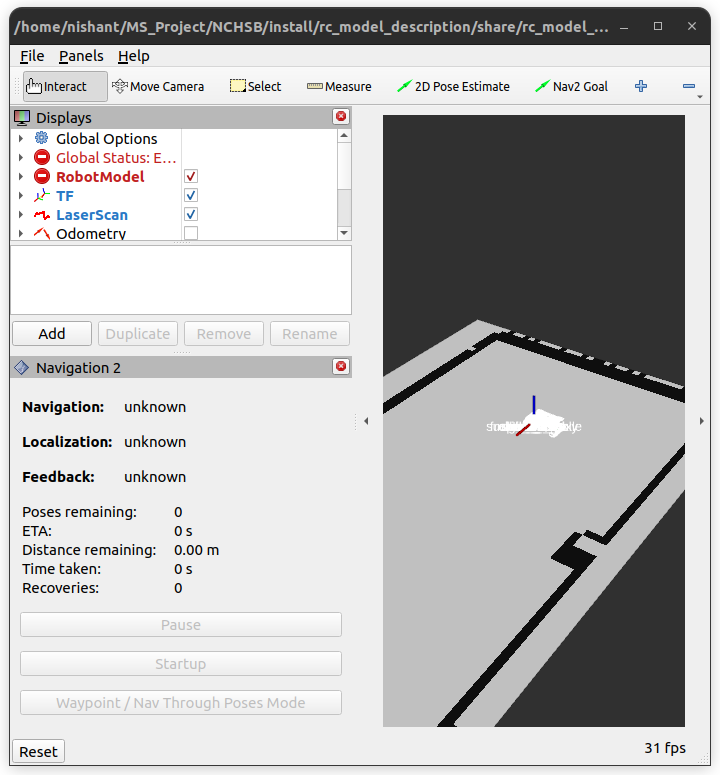
\includegraphics[width=0.7\textwidth]{smoke_test1_no_robot_no_lidar.png}
  \caption{Smoke test 1: RViz shows Global Status error, no robot model, no LiDAR
    points.  Map loads but TF tree is broken and scan topic has no data.}
  \label{fig:smoke1}
\end{figure}

\logentry{Root Cause Analysis (cascade)}
\begin{enumerate}
  \item \textbf{Gazebo starts paused}: The \texttt{gz\_sim.launch.py} was called
    with only the world path as \texttt{gz\_args}.  Without \texttt{-r} (run),
    Gazebo starts in a paused state --- physics never ticks.  Evidence: controller
    manager logged \texttt{gazebo simulation period (0 s)}.
  \item \textbf{Controllers cannot activate}: The \texttt{gz\_ros2\_control}
    hardware interface needs at least one physics step to report joint states.
    With period = 0, the switch request blocks until the 5\,s timeout.
  \item \textbf{No odometry}: Ackermann controller never activated, so \texttt{/odom}
    is never published.
  \item \textbf{EKF starved}: \texttt{robot\_localization} receives no \texttt{/odom}
    messages, so it never publishes the \texttt{odom $\to$ base\_link} TF.
  \item \textbf{Nav2 blocked}: Costmap activation requires \texttt{odom} frame
    in TF.  Without it, the activation loop spins forever.
  \item \textbf{No LiDAR}: \texttt{gpu\_lidar} sensor doesn't produce scans when
    physics is paused (update depends on sim steps).
  \item \textbf{RViz blank}: No TF tree $\Rightarrow$ robot model cannot be
    displayed; no scan data $\Rightarrow$ no red points.
\end{enumerate}

\logentry{Fixes Applied}
\begin{enumerate}
  \item \textbf{Auto-run Gazebo}: Changed \texttt{gz\_args} from
    \texttt{world\_path} to \texttt{['-r ', world\_path]} in
    \texttt{fortress\_bringup.launch.py}.  The \texttt{-r} flag starts
    Gazebo's physics loop immediately.
  \item \textbf{Increased controller spawner timeouts}: Added
    \texttt{--controller-manager-timeout 30} to both spawner argument lists.
    Raised \texttt{TimerAction} delays: robot spawn at 2\,s, JSB spawner at
    8\,s, Ackermann spawner at 10\,s (was 1/3/4.5\,s).
  \item \textbf{Increased Nav2 / goal\_sender delays}: Nav2
    \texttt{bringup\_launch.py} now starts at $t+15$\,s (was 8\,s);
    \texttt{goal\_sender} at $t+30$\,s (was 15\,s), giving controllers time
    to fully activate and odometry to flow.
  \item \textbf{Fixed \texttt{rclpy.shutdown()} crash}: All four Python nodes
    (\texttt{pedestrian\_driver}, \texttt{gt\_collision\_detector},
    \texttt{gt\_people\_publisher}, \texttt{goal\_sender}) now guard shutdown
    with \texttt{if rclpy.ok():} and catch
    \texttt{rclpy.executors.ExternalShutdownException}.  This prevents the
    ``already called'' crash when the ROS\,2 signal handler shuts down the
    context before the \texttt{finally} block.
\end{enumerate}

\logentry{Full TF Chain Analysis}
The expected TF chain for the full Nav2 stack to work is:
\begin{verbatim}
map --> odom --> base_link --> chassis_link --> lidar_link
  |       |           |
 AMCL    EKF      robot_state_publisher (static)
\end{verbatim}
Each link and its dependencies:
\begin{enumerate}
  \item \texttt{base\_link $\to$ chassis\_link $\to$ lidar\_link} (and all other
    robot links): Published by \texttt{robot\_state\_publisher} from
    \texttt{/robot\_description}.  This works independently of everything else.
    \textbf{Status in log}: Working (lines 16--31: all segments loaded).
  \item \texttt{odom $\to$ base\_link}: Published by EKF
    (\texttt{robot\_localization/ekf\_node}).  Requires input from
    \texttt{/odom} topic (Ackermann controller output).
    \textbf{Status in log}: Not working.  EKF has no input because Ackermann
    controller never activated.
  \item \texttt{map $\to$ odom}: Published by AMCL after it localizes the robot
    in the static map.  Requires: (a) \texttt{/scan} data, (b)
    \texttt{odom $\to$ base\_link} TF (to transform scans into the odom frame),
    (c) the static map from \texttt{map\_server}.
    \textbf{Status in log}: Not working.  AMCL loaded the map (line 215:
    ``Received a 405 $\times$ 48 map'') but could not transform scans.  Line 318:
    ``\texttt{Message Filter dropping message: frame 'lidar\_link'}\ldots{}
    \texttt{queue is full}'' --- scan messages pile up because TF from
    \texttt{lidar\_link} to \texttt{odom} does not exist.
\end{enumerate}

\noindent The break point is step 2: without the Ackermann controller running
(because Gazebo was paused), the entire TF chain from \texttt{odom} upward is
broken.

\begin{figure}[htbp]
  \centering
  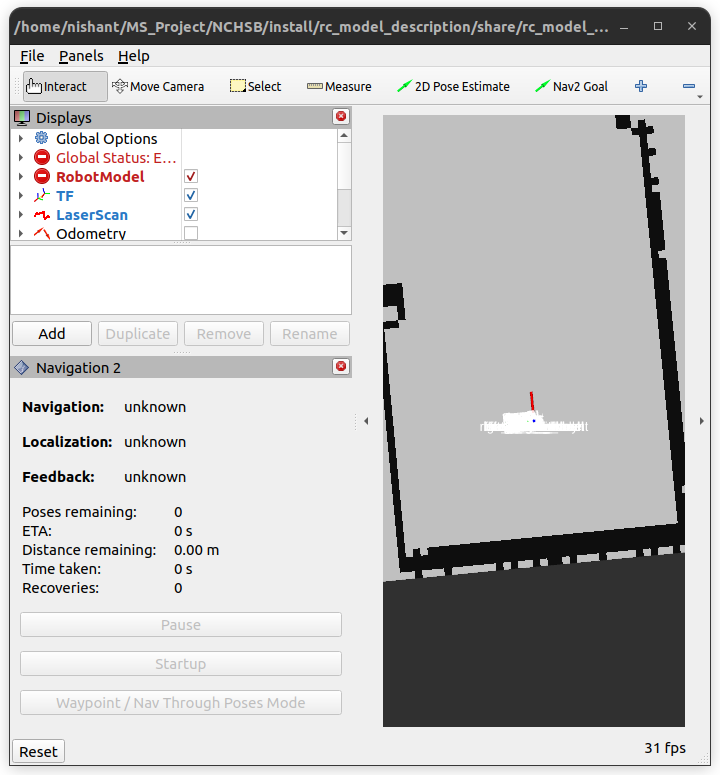
\includegraphics[width=0.7\textwidth]{smoke_test2_map_loaded_no_scan.png}
  \caption{Smoke test 2: Map loads (corridor\_straight with wall features visible),
    robot model partially visible, but Global Status error persists.  No LiDAR
    scan points due to broken \texttt{odom $\to$ base\_link} TF.  Navigation and
    Localization status both ``unknown.''}
  \label{fig:smoke2}
\end{figure}

\logentry{Secondary Issue: AMCL Message Filter Queue Full}
Log line 318: \texttt{[amcl]: Message Filter dropping message: frame
'lidar\_link' at time 2.120 for reason 'discarding message because the queue
is full'}.  This occurs because:
\begin{itemize}
  \item AMCL's message filter waits for the TF from \texttt{lidar\_link} to
    \texttt{odom} before processing each scan.
  \item Without \texttt{odom $\to$ base\_link}, the transform never becomes
    available.
  \item Scan messages accumulate in the filter's queue until it overflows.
  \item RViz shows the same symptom (line 319).
\end{itemize}
This is a \emph{consequence} of the paused Gazebo root cause, not a separate
bug.

\logentry{Secondary Issue: \texttt{rclpy.shutdown()} Double-Call Crash}
On Ctrl-C, all four Python nodes (\texttt{pedestrian\_driver},
\texttt{gt\_collision\_detector}, \texttt{gt\_people\_publisher},
\texttt{goal\_sender}) crashed with:
\begin{verbatim}
rclpy._rclpy_pybind11.RCLError: failed to shutdown:
  rcl_shutdown already called on the given context
\end{verbatim}
This happens because the ROS\,2 launch system's signal handler calls
\texttt{rclpy.shutdown()} on SIGINT before the nodes' \texttt{finally} blocks
execute.  The fix adds \texttt{if rclpy.ok():} guards and catches
\texttt{ExternalShutdownException}.

\logentry{Verification}
After applying fixes, the installed launch file was verified to contain:
\begin{itemize}
  \item \texttt{gz\_args: ['-r ', world\_path]} --- auto-run
  \item \texttt{--controller-manager-timeout 30} --- both spawners
  \item \texttt{TimerAction} delays: 2\,s / 8\,s / 10\,s --- spawn / JSB / Ackermann
  \item Nav2 at $t+15$\,s, goal\_sender at $t+30$\,s
  \item \texttt{tf\_odometry} remapping confirmed absent from installed xacro
    (only present as a comment explaining why it was removed)
\end{itemize}

% ------------------------------------------------------------------

\subsection*{8.5 Deeper Smoke Test Analysis --- Three Remaining Issues}

After fixing the paused-Gazebo root cause (\S8.4), the controllers activated
(confirmed: \texttt{/odom} at $\sim$4\,Hz, \texttt{/odometry/filtered}
present), but the robot still did not appear in RViz and \texttt{/tracked\_people}
carried no data.  Running SLAM Toolbox instead of Nav2 \emph{did} show the
robot and LiDAR correctly (Figure~\ref{fig:smoke3}), proving the TF chain
\texttt{odom $\to$ base\_link} was intact.  Three additional issues were
identified.

\begin{figure}[htbp]
  \centering
  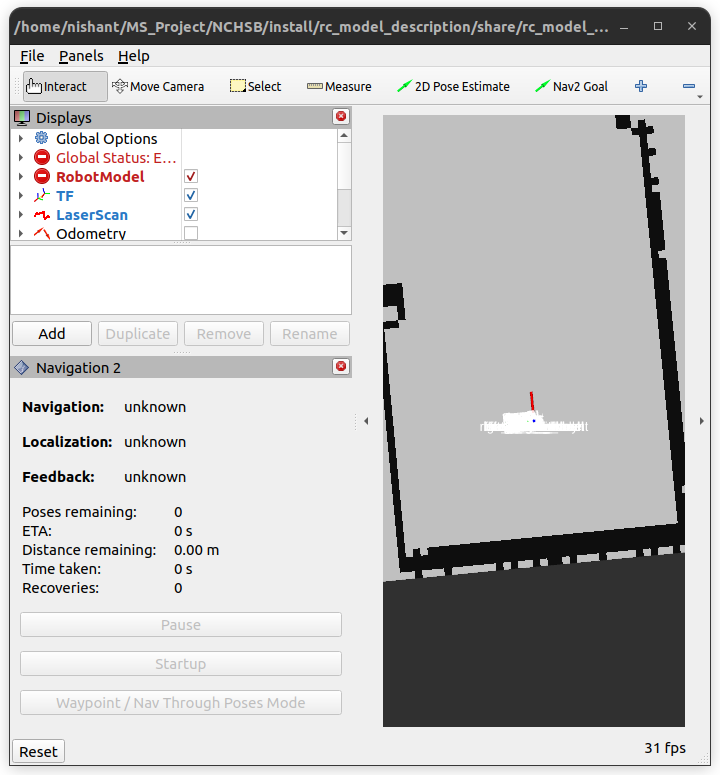
\includegraphics[width=0.7\textwidth]{smoke_test3_slam_works_nav2_no_localize.png}
  \caption{SLAM Toolbox run alongside the smoke test.  The robot model,
    LiDAR points, and inflation layer are all visible because SLAM Toolbox
    provides \texttt{map $\to$ odom} directly.  Nav2's AMCL does not.}
  \label{fig:smoke3}
\end{figure}

\subsubsection*{Issue A: AMCL Missing Initial Pose}

\logentry{Symptom}
RViz showed the map but no robot, no scan, and Navigation / Localization status
``unknown.''  SLAM Toolbox worked because it provides \texttt{map $\to$ odom}
from scan matching --- no initial pose needed.

\logentry{Root Cause}
Nav2's AMCL requires an initial pose hypothesis before it starts publishing
\texttt{map $\to$ odom}.  By default it waits for a \texttt{/initialpose}
message (the ``2D Pose Estimate'' button in RViz).  Our Nav2 configs did not
set \texttt{set\_initial\_pose: true}, so AMCL never localized.

\logentry{Fix}
Added to \emph{all four} Nav2 config files
(\texttt{nav2\_mppi\_vanilla.yaml}, \texttt{nav2\_mppi\_social\_instant.yaml},
\texttt{nav2\_mppi\_social\_pred.yaml}, \texttt{nav2\_full.yaml}):
\begin{verbatim}
amcl:
  ros__parameters:
    set_initial_pose: true
    initial_pose:
      x: 0.0
      y: 0.0
      z: 0.0
      yaw: 0.0
\end{verbatim}
The initial pose $(0,0,0)$ matches the robot's spawn location in the SLAM-generated
map coordinate frame.  AMCL will converge from this prior on the first few scans.

\subsubsection*{Issue B: Pedestrian Models Never Spawned}

\logentry{Symptom}
\texttt{pedestrian\_driver} logged ``\texttt{pedestrian\_1 started moving}'' but
\texttt{ros2 topic echo /tracked\_people --once} returned no data.

\logentry{Root Cause}
\texttt{pedestrian\_driver.py} calls \texttt{set\_pose} to \emph{move} a model
named \texttt{pedestrian\_1}, but \textbf{nobody spawns that model into Gazebo}.
The spawn command (\texttt{ros2 run ros\_gz\_sim create -file model.sdf -name
pedestrian\_1 \ldots}) was missing from \texttt{sim\_experiment.launch.py}.

The \texttt{set\_pose} service silently ignores requests for non-existent
entities --- no error is logged, the pedestrian just never appears.

\logentry{Fix}
Added \texttt{\_spawn\_pedestrians()} OpaqueFunction to
\texttt{sim\_experiment.launch.py}.  It:
\begin{enumerate}
  \item Parses the \texttt{pedestrians\_json} LaunchConfiguration.
  \item For each pedestrian, spawns a \texttt{pedestrian/model.sdf} cylinder
    into Gazebo at the first waypoint position using
    \texttt{ros2 run ros\_gz\_sim create}.
  \item Runs at $t+5$\,s via TimerAction (after Gazebo world loads but before
    Nav2 starts).
\end{enumerate}

\subsubsection*{Issue C: \texttt{/tracked\_people} and
  \texttt{/min\_human\_distance} Empty}

\logentry{Symptom}
\texttt{ros2 topic echo /tracked\_people --once} hung indefinitely.
\texttt{ros2 topic echo /min\_human\_distance --once} also hung.

\logentry{Root Cause}
This is a \emph{consequence} of Issue B.  The data dependency chain is:
\begin{verbatim}
pedestrian model in Gazebo
  --> dynamic_pose bridge publishes TF for pedestrian_* frames
    --> gt_people_publisher filters for pedestrian_ prefix
      --> publishes /tracked_people
        --> gt_collision_detector computes distances
          --> publishes /min_human_distance
\end{verbatim}
Since no pedestrian model existed in Gazebo, the \texttt{dynamic\_pose} bridge
had nothing to publish, so the entire chain was empty.

\logentry{Fix}
Resolved by Issue B fix (spawning pedestrian models).

\logentry{Topic Verification (pre-fix)}
The topic list confirmed all topics \emph{existed} but most carried no data:
\begin{verbatim}
/scan                        ✓  (~4 Hz)
/odom                        ✓
/odometry/filtered           ✓
/tracked_people              exists, no data
/min_human_distance          exists, no data
/collision_event             exists, no data
/trial_result                exists, no data
\end{verbatim}

% ------------------------------------------------------------------

\subsection*{8.6 Smoke Test 4 --- Near-Success, Goal Sender Timing Race}

After applying fixes from \S8.4 and \S8.5, the smoke test achieved:
\begin{itemize}
  \item Gazebo running with \texttt{-r} flag ($\text{sim period}=0.001$\,s)
  \item Both controllers activated cleanly (no timeouts)
  \item Pedestrian cylinder spawned and visible in Gazebo
    (Figure~\ref{fig:smoke4_gz})
  \item AMCL localized with auto-set initial pose
  \item All Nav2 managed nodes active with bond timers
  \item LiDAR scans visible in RViz (Figure~\ref{fig:smoke4_rviz1})
  \item Nav2 costmaps, global path, and inflation layer all visible
    (Figure~\ref{fig:smoke4_rviz2})
  \item \texttt{/tracked\_people} publishing data with correct pedestrian position
  \item \texttt{/min\_human\_distance} returning $\sim$9.0\,m (robot at $x{=}{-}9$,
    pedestrian at $x{=}9$)
\end{itemize}

\begin{figure}[htbp]
  \centering
  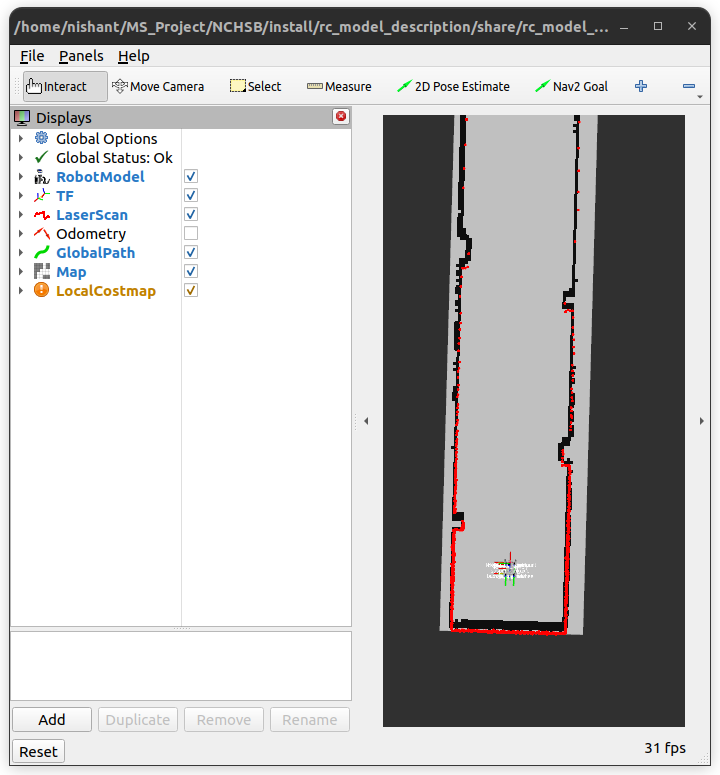
\includegraphics[width=0.48\textwidth]{smoke_test4_lidar_scans_loaded.png}
  \hfill
  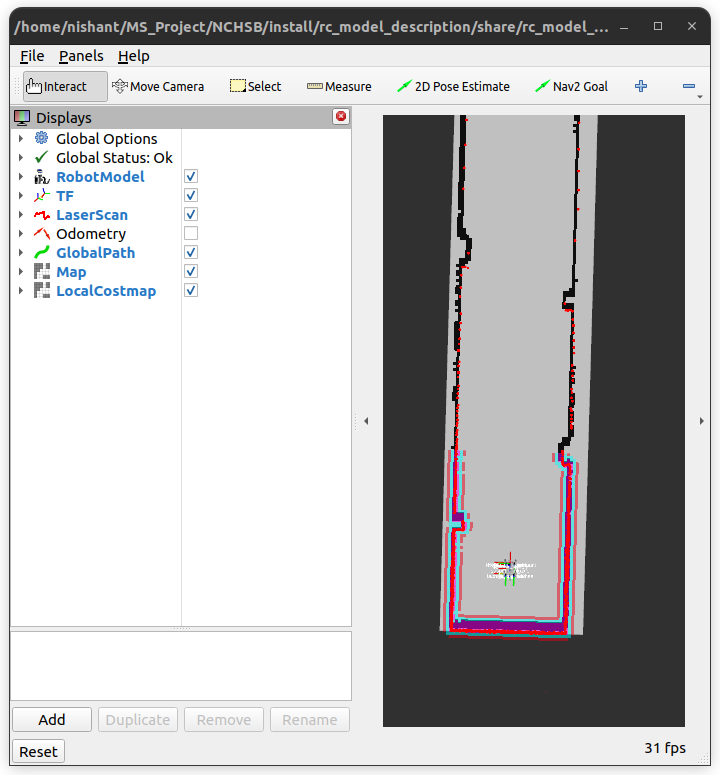
\includegraphics[width=0.48\textwidth]{smoke_test4_nav2_costmap_path.png}
  \caption{Left (Figure~\ref{fig:smoke4_rviz1}): RViz showing robot model,
    LiDAR scans (red), and map with Global Status OK.  Right
    (Figure~\ref{fig:smoke4_rviz2}): Nav2 costmaps loaded with inflation layer
    (cyan/magenta), global path (green), and local costmap.}
  \label{fig:smoke4_rviz1}
  \label{fig:smoke4_rviz2}
\end{figure}

\begin{figure}[htbp]
  \centering
  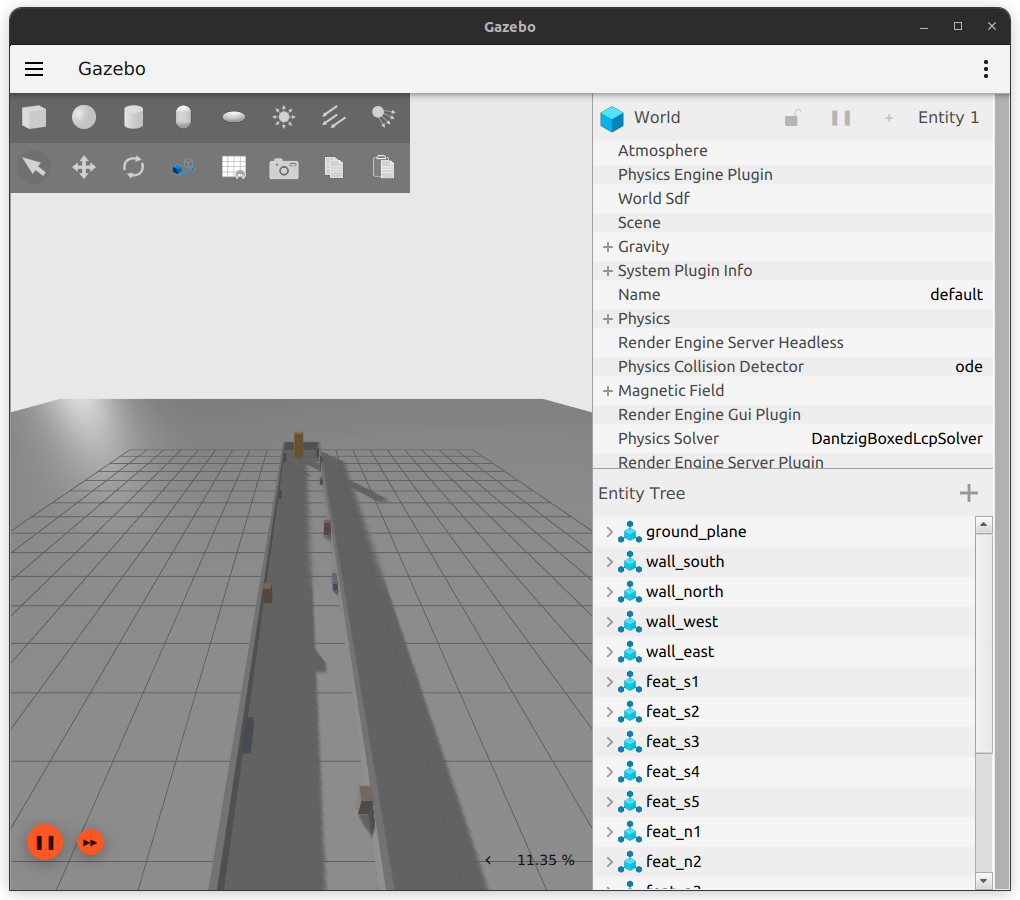
\includegraphics[width=0.7\textwidth]{smoke_test4_pedestrian_in_gazebo.png}
  \caption{Gazebo view showing the corridor\_straight world with wall features
    (brown box protrusions) and the spawned pedestrian cylinder visible in the
    corridor.  Entity tree confirms world structure.}
  \label{fig:smoke4_gz}
\end{figure}

\logentry{Single Remaining Failure: Goal Sender Timing Race}
The robot did not move because the \texttt{goal\_sender} timed out before Nav2
was ready:
\begin{verbatim}
[goal_sender] Action server not available after 30s
[goal_sender] Published trial result: TIMEOUT_NO_SERVER
\end{verbatim}

Timeline analysis (all times relative to launch):
\begin{itemize}
  \item $t{+}30$\,s: \texttt{goal\_sender} starts, begins
    \texttt{wait\_for\_server(30s)}
  \item $t{+}60$\,s: \texttt{goal\_sender} gives up
    (\texttt{TIMEOUT\_NO\_SERVER})
  \item $t{+}65$\,s: \texttt{bt\_navigator} finishes activating (creates
    \texttt{navigate\_to\_pose} action server)
\end{itemize}
The goal sender missed the action server by $\sim$5 seconds.

\logentry{Fix}
\begin{enumerate}
  \item Increased \texttt{goal\_sender} launch delay from 30\,s to 45\,s in
    \texttt{sim\_experiment.launch.py}.
  \item Increased \texttt{wait\_for\_server} timeout from 30\,s to 60\,s in
    \texttt{goal\_sender.py}.
  \item Combined: goal sender now starts at $t{+}45$\,s and waits until
    $t{+}105$\,s if needed.  Nav2 activation at $\sim t{+}65$\,s is well
    within this window.
\end{enumerate}

\logentry{Secondary Fix: Stale Build Files}
The \texttt{rclpy.shutdown()} guard fix from \S8.4 was not picked up by
\texttt{colcon build --symlink-install}.  For ament\_python packages, the
build directory may contain copies rather than symlinks.  Fixed by deleting
\texttt{build/} and \texttt{install/} for the bringup package and rebuilding
from clean.  Verified with \texttt{grep} that the build directory now contains
the \texttt{rclpy.ok()} guard.

\logentry{Pedestrian Movement Verification}
Log confirmed:
\begin{verbatim}
[pedestrian_driver] pedestrian_1 started moving (delay=1.0s)
... (117s wall clock later) ...
[pedestrian_driver] pedestrian_1 reached final waypoint
\end{verbatim}
The pedestrian traversed the full 18\,m corridor at 1.1\,m/s in sim time.
Wall clock time was $\sim$117\,s due to Gazebo running at $\sim$11\% real-time
speed (typical for GPU LiDAR simulation on desktop hardware).

% ------------------------------------------------------------------

\subsection*{8.7 Smoke Test 5 --- Goal Rejected During Nav2 Initialization}

Everything from Smoke Test~4 continued to work (Gazebo running, controllers,
pedestrian spawned and moving, AMCL localized, all topics publishing).
However the goal was \textbf{REJECTED} by Nav2.

\logentry{Root Cause: bt\_navigator Lifecycle Race}
Nav2's \texttt{bt\_navigator} creates the \texttt{navigate\_to\_pose} action
server during its \textbf{configure} lifecycle phase, but only \emph{accepts}
goals after its \textbf{activate} phase.  The \texttt{lifecycle\_manager\_navigation}
transitions nodes sequentially:
\texttt{controller\_server} $\to$ \texttt{smoother\_server} $\to$
\texttt{planner\_server} $\to$ \texttt{behavior\_server} $\to$
\texttt{bt\_navigator} $\to$ \texttt{waypoint\_follower} $\to$
\texttt{velocity\_smoother}.

Timeline (wall clock seconds from launch):
\begin{center}
\begin{tabular}{rl}
$t{+}58.3$\,s & \texttt{bt\_navigator} begins \emph{Configuring}
  (action server created) \\
$t{+}58.6$\,s & \texttt{goal\_sender} discovers action server, sends goal \\
$t{+}58.8$\,s & \textbf{Goal REJECTED} (bt\_navigator not yet active) \\
$t{+}59.9$\,s & \texttt{bt\_navigator} \emph{Activating} (would now accept goals) \\
\end{tabular}
\end{center}

\logentry{Fix: Goal Sender Retry Logic}
Rewrote \texttt{goal\_sender.py} with a retry mechanism:
\begin{itemize}
  \item After \texttt{wait\_for\_server(60s)} succeeds, send goal via
    \texttt{\_attempt\_send\_goal()}.
  \item If \texttt{goal\_response\_cb} sees rejection and retries remain
    ($\text{max}=10$), schedule a retry after 3\,s using a one-shot timer.
  \item Cancel the retry timer before re-sending to prevent duplicate sends.
  \item Added \texttt{\_done} flag to prevent multiple result publications
    during shutdown races.
\end{itemize}

\logentry{Fix: rclpy.shutdown() Race Condition}
The \texttt{if rclpy.ok(): rclpy.shutdown()} pattern has a TOCTOU race:
\texttt{rclpy.ok()} returns True, then the SIGINT signal handler calls
\texttt{rclpy.shutdown()} on another thread, and our code's subsequent
\texttt{rclpy.shutdown()} call fails.  Fixed all four Python nodes
(\texttt{goal\_sender}, \texttt{pedestrian\_driver},
\texttt{gt\_people\_publisher}, \texttt{gt\_collision\_detector}) to wrap
\texttt{destroy\_node()} and \texttt{rclpy.shutdown()} in separate
\texttt{try/except Exception} blocks.

Clean-rebuilt the bringup package (deleted \texttt{build/} and
\texttt{install/} directories) and verified fixes in the build directory.

% ------------------------------------------------------------------

\subsection*{8.8 Smoke Test 6 --- Empty Behavior Tree}

The goal sender retry logic worked: goal accepted on attempt~2.  However the
goal was immediately \textbf{ABORTED}:
\begin{verbatim}
[BehaviorTreeEngine]: Behavior tree threw exception:
    Empty Tree. Exiting with failure.
[bt_navigator]: Goal failed
\end{verbatim}

\logentry{Root Cause}
All four Nav2 config YAMLs had \texttt{default\_nav\_to\_pose\_bt\_xml: ""}
(empty string).  In Nav2~Humble, an explicit empty string overrides the
built-in default behavior tree.  The \texttt{bt\_navigator} loads an empty
XML, producing the ``Empty Tree'' error.

\logentry{Fix}
Set the BT XML paths to Nav2's default behavior trees in all five config
files:
\begin{verbatim}
default_nav_to_pose_bt_xml:
  /opt/ros/humble/share/nav2_bt_navigator/behavior_trees/
  navigate_to_pose_w_replanning_and_recovery.xml
default_nav_through_poses_bt_xml:
  /opt/ros/humble/share/nav2_bt_navigator/behavior_trees/
  navigate_through_poses_w_replanning_and_recovery.xml
\end{verbatim}

% ------------------------------------------------------------------

\subsection*{8.9 Smoke Test 7 --- cmd\_vel Topic Mismatch (Robot Not Moving)}

The behavior tree fix resolved the ABORTED error.  Nav2 accepted the goal,
computed a global path (visible in RViz), and the controller\_server began
computing velocity commands.  However the robot never physically moved.
After $\sim$130\,s wall clock, the progress checker fired:
\begin{verbatim}
[controller_server]: Failed to make progress
\end{verbatim}

\logentry{Root Cause: cmd\_vel Topic Disconnect}
Nav2's \texttt{navigation\_launch.py} uses these remappings:
\begin{center}
\begin{tabular}{lll}
\textbf{Node} & \textbf{Publishes to} & \textbf{Subscribes from} \\
\hline
controller\_server & \texttt{/cmd\_vel\_nav} & --- \\
velocity\_smoother & \texttt{/cmd\_vel} & \texttt{/cmd\_vel\_nav} \\
\hline
ackermann\_steering\_controller & --- & \texttt{/.../reference\_unstamped} \\
\end{tabular}
\end{center}
The velocity\_smoother was publishing to \texttt{/cmd\_vel}, but the
ackermann\_steering\_controller subscribed to its own namespaced topic
\texttt{/ackermann\_steering\_controller/reference\_unstamped}.
\textbf{No node was listening to Nav2's output.}

\logentry{Fix}
Added a remapping in \texttt{gazebo\_control.xacro} inside the
\texttt{GazeboSimROS2ControlPlugin} \texttt{<ros>} block:
\begin{verbatim}
<remapping>ackermann_steering_controller/reference_unstamped
    :=cmd_vel</remapping>
\end{verbatim}
This causes the controller to subscribe to \texttt{/cmd\_vel} instead of its
default namespaced topic, completing the topic chain:
\begin{verbatim}
controller_server → /cmd_vel_nav → velocity_smoother → /cmd_vel
    → ackermann_steering_controller
\end{verbatim}

% ------------------------------------------------------------------

\subsection*{8.10 Shutdown Behavior Summary}

\logentry{Current Shutdown Flow}
\begin{enumerate}
  \item \texttt{goal\_sender} publishes trial result to \texttt{/trial\_result}
    $\to$ calls \texttt{rclpy.shutdown()} $\to$ process exits cleanly.
  \item \texttt{metrics\_logger} receives trial result $\to$ writes CSV
    $\to$ calls \texttt{rclpy.shutdown()} $\to$ process exits cleanly.
  \item \textbf{All other processes keep running} (Gazebo, Nav2, bridges,
    collision detector, pedestrian driver) because no process is marked
    \texttt{required} in the launch file for auto-shutdown.
  \item User must \texttt{Ctrl+C} to terminate the launch system.
  \item On SIGINT, the launch system sends SIGINT to all child processes.
    Some (especially the Nav2 composable container) require escalation to
    SIGTERM and eventually SIGKILL, which is normal.
\end{enumerate}

\logentry{Shutdown Errors (All Cosmetic, Do Not Affect Trial Data)}
\begin{itemize}
  \item \textbf{RViz exit code -11 (SIGSEGV)}: Common crash when Gazebo shuts
    down and the rendering pipeline loses resources. Harmless.
  \item \textbf{Nav2 container SIGKILL escalation}: The composable container
    with $\sim$12 lifecycle nodes takes longer than 5\,s to deactivate.
    Launch escalates SIGINT $\to$ SIGTERM $\to$ SIGKILL. Harmless.
  \item \textbf{gt\_collision\_detector RuntimeError}: rclpy Humble race
    condition where \texttt{take\_message()} is called on an invalidated DDS
    handle during shutdown. Fixed by catching \texttt{RuntimeError} in the
    \texttt{except} clause.
  \item \textbf{``Failed to publish log message to rosout''}: Nodes try to log
    after their ROS context is invalidated. Cosmetic.
  \item \textbf{pedestrian\_driver / gt\_people\_publisher exit code 1}:
    Fixed by wrapping \texttt{rclpy.shutdown()} in \texttt{try/except}.
\end{itemize}

\logentry{For Automated Experiments}
The \texttt{run\_experiment.py} script launches \texttt{sim\_experiment.launch.py}
as a subprocess and monitors \texttt{/trial\_result} (or uses a wall-clock
timeout). When the trial ends, it sends SIGINT to the launch subprocess,
collects the CSV, and proceeds to the next trial. Manual \texttt{Ctrl+C} is
not needed in automated mode.

% ------------------------------------------------------------------

\subsection*{8.11 Smoke Test Progress Summary (End of Day 2)}

\logentry{What Works}
\begin{itemize}
  \item Gazebo launches with \texttt{-r} flag (not paused), physics at 0.001\,s
    period
  \item Robot spawns, \texttt{ros2\_control} activates both controllers
    (joint\_state\_broadcaster + ackermann\_steering\_controller)
  \item Pedestrian cylinder model spawns into Gazebo and moves along waypoints
  \item EKF publishes \texttt{odom $\to$ base\_link} transform
  \item AMCL auto-localizes with \texttt{set\_initial\_pose: true}, publishes
    \texttt{map $\to$ odom} transform
  \item All Nav2 lifecycle nodes activate (map\_server, amcl, controller\_server,
    planner\_server, bt\_navigator, behavior\_server, velocity\_smoother,
    waypoint\_follower)
  \item Behavior tree loads successfully (\texttt{navigate\_to\_pose\_w\_replanning\_and\_recovery.xml})
  \item Goal sender retries on rejection, goal accepted on attempt 2
  \item Global path computed and visible in RViz
  \item MPPI controller computes velocity commands at $\sim$20\,Hz (with
    occasional rate misses due to CPU load)
  \item \texttt{cmd\_vel} remapping connects Nav2 output to ackermann controller
    (confirmed: deprecation warnings show controller receiving Twist messages
    at $\sim$20\,Hz from goal acceptance onward)
  \item \texttt{/tracked\_people} publishes pedestrian data correctly
  \item \texttt{/min\_human\_distance} reports correct distances
  \item Metrics logger writes CSV with partial data on interrupt
  \item Odometry reports \texttt{path\_length\_m: 8.172} --- robot IS moving
  \item LiDAR scans, costmaps, and inflation layers all visible in RViz
\end{itemize}

\logentry{Remaining Verification (Tomorrow)}
\begin{itemize}
  \item \textbf{Visual confirmation of robot motion}: User did not visually
    observe the robot moving in Gazebo/RViz despite log evidence of 8.172\,m
    path. Need to verify with \texttt{ros2 topic echo /odom} that position
    changes over time. Possible causes: slow Gazebo RTF ($\sim$11\%), camera
    angle, or an undiagnosed issue.
  \item \textbf{Full trial completion}: Let the smoke test run to completion
    without Ctrl+C. At $\sim$11\% RTF, the 60\,s sim-time timeout needs
    $\sim$9 minutes of wall clock time.
  \item \textbf{Pedestrian timing}: Pedestrian finishes traversal before robot
    starts navigating (pedestrian moves in sim time, which elapses even during
    Nav2 initialization). Consider increasing \texttt{start\_delay} or using a
    longer pedestrian trajectory.
  \item \textbf{Automated shutdown}: Add a mechanism so the launch
    auto-terminates after \texttt{metrics\_logger} writes the CSV (e.g., mark
    \texttt{metrics\_logger} as a required process, or add a shutdown event
    handler).
  \item \textbf{Clean exit}: Verify all Python nodes exit cleanly after
    \texttt{RuntimeError} catch and \texttt{try/except} shutdown fixes.
  \item \textbf{SLAM maps for other corridors}: Generate maps for L-turn,
    T-junction, narrow, wide, and loop corridors.
\end{itemize}

% ============================================================

\section*{Day 3: Pedestrian Timing, Inflation, Auto-Shutdown}

\logentry{Session Overview}
Day 3 focused on completing Priority 1--4: verify robot motion, full trial
completion, fix pedestrian timing, and add auto-shutdown. All four were
completed. Additional work: inflation radius tuning for corridor geometry,
and discussion of lateral offset distribution for stronger experimental design.

% ------------------------------------------------------------------

\subsection*{9.1 Priority 1: Verify Robot Motion}

\logentry{Test}
User ran smoke test with \texttt{mppi\_vanilla} on \texttt{corridor\_straight}.
RViz Nav2 panel showed: \texttt{Navigation: active}, \texttt{Localization: active},
\texttt{Feedback: reached}, \texttt{Distance remaining: 0.00\,m}.

\logentry{Result}
Robot navigated from spawn (-9, 0) to goal (9, 0) successfully. Odometry samples
at two time points showed timestamps changing (13\,s $\to$ 18\,s sim-time).
\textbf{Priority 1 confirmed.}

% ------------------------------------------------------------------

\subsection*{9.2 Priority 2: Full Trial Completion}

\logentry{Result}
Same run confirmed full trial completion: \texttt{Goal SUCCEEDED in 9.3\,s},
\texttt{path\_length\_m: 8.635}, \texttt{collision\_count: 0}, CSV written with
all fields. \textbf{Priority 2 confirmed.}

% ------------------------------------------------------------------

\subsection*{9.3 Priority 3: Fix Pedestrian Timing}

\logentry{Problem}
Pedestrian cylinder spawned and driver logic ran (logs showed ``pedestrian\_1
started moving'', ``reached final waypoint''), but the cylinder did \emph{not}
physically move in Gazebo. User reported: ``I don't see the orange cylinder
that we kept as a person moving. It is in the same place.''

\logentry{Iteration 1: Signal-Based Timing}
Added \texttt{/trial\_active} topic: \texttt{goal\_sender} publishes
\texttt{std\_msgs/Empty} when goal is accepted; \texttt{pedestrian\_driver}
subscribes and only starts its movement timer after receiving the signal.
This fixed the timing mismatch (pedestrian used to finish before robot started).
Logs confirmed: \texttt{Received /trial\_active}, \texttt{pedestrian\_1 started
moving (delay=1.0s)}. But the cylinder still did not move visually.

\logentry{Iteration 2: Root Cause}
\texttt{pedestrian\_driver} used \texttt{ros\_gz\_interfaces.srv.SetEntityPose}
to call \texttt{/world/default/set\_pose}. The \texttt{ros\_gz\_bridge} for
Humble/Fortress bridges \emph{topics} only, not \emph{services}. The ROS 2
service client had no server; \texttt{service\_is\_ready()} always returned
False; \texttt{\_set\_pose()} returned silently every time. The driver's
internal state advanced (waypoints, ``reached final waypoint'') but no pose
updates reached Gazebo.

\logentry{Iteration 3: Fix}
Replaced ROS service call with \texttt{subprocess.Popen} invoking \texttt{ign
service -s /world/default/set\_pose --reqtype ignition.msgs.Pose --reptype
ignition.msgs.Boolean --req} with a Pose message (name, position x/y/z).
Non-blocking: if previous call still
running, skip (natural rate limiting). No Python Ignition transport bindings
available; subprocess is the pragmatic solution.

\logentry{Result}
Pedestrian cylinder now physically moves in Gazebo. User confirmed: ``the bot
moves and the person moves.'' \textbf{Priority 3 complete.}

% ------------------------------------------------------------------

\subsection*{9.4 Inflation Radius Tuning}

\logentry{User Feedback}
``The bot is colliding with the person, it needs to stop or either take another
part right?'' With 0.09\,m inflation, robot plowed through pedestrian
(\texttt{min\_separation\_m: 0.446}, \texttt{collision\_count: 1}).

\logentry{Geometry Analysis}
\begin{itemize}
  \item Corridor: walls at y = $\pm$0.95\,m $\Rightarrow$ usable width 1.9\,m
  \item Robot footprint: 0.30\,m $\times$ 0.16\,m
  \item Pedestrian cylinder: diameter 0.50\,m (radius 0.25\,m)
  \item Current inflation\_radius: 0.09\,m (local), 0.08\,m (global)
  \item Total keep-away from pedestrian center: 0.25 + 0.09 = 0.34\,m
  \item Robot needs 0.15 + 0.25 = 0.40\,m to avoid physical contact
  \item 0.09\,m inflation is too small --- MPPI doesn't ``see'' danger until
    practically touching
\end{itemize}

\logentry{User Question}
``Do we need to have an inflation radius that matches [corridor width minus
robot width]?'' Discussion: inflation must be large enough for MPPI to react,
but small enough that a feasible path exists. With 0.55\,m (Nav2 default),
passable width shrinks to $\sim$0.30\,m --- robot may get stuck.

\logentry{Decision}
Set \texttt{inflation\_radius: 0.25} in all 5 Nav2 configs (local and global
costmap). At 0.25\,m, passable width $\sim$0.60\,m --- robot can squeeze past
comfortably. Fair baseline for paper (reviewers won't cry strawman).

\logentry{Result After 0.25\,m Inflation}
User: ``the bot actually stopped and the human was the one who came and crashed
into the bot.'' Metrics: \texttt{collision\_count: 1}, \texttt{min\_separation\_m:
0.394}, \texttt{stuck\_time\_s: 11.25}. Robot saw inflated pedestrian, stopped,
waited; pedestrian walked into stationary robot. This is the expected vanilla
baseline --- perfect for paper comparison.

% ------------------------------------------------------------------

\subsection*{9.5 Lateral Offset Distribution (Discussion)}

\logentry{User Feedback}
``The corridor is about x\,m wide, the bot is about y\,m. Humans will walk along
(x-y), and they will only have this space. Is there enough distance for the bot
to change track? Both are moving in the centre. Which will be a stronger study:
if both in the centre, or if both in the side? Like 2 humans walking in the
corridor, both are not walking in the centre, one keeps to the left lane and
the other to the right lane, but this should not be hardcoded coz movement in
corridors can be unpredictable.''

\logentry{Response}
\begin{itemize}
  \item 18\,m corridor gives $\sim$9\,s before encounter --- plenty of time.
  \item Current \texttt{lateral\_offset: mean: 0.15} puts pedestrian near center.
  \item Real humans keep $\sim$0.3--0.5\,m from wall (``lane'' behavior).
  \item Suggested: \texttt{mean: 0.35, std: 0.15, min: -0.1, max: 0.7} for
    realistic distribution across trials.
  \item Stronger study: range of difficulties (head-on center vs own lane).
  \item Not implemented yet --- user said ``let us test this'' (Priority 4).
\end{itemize}

% ------------------------------------------------------------------

\subsection*{9.6 Priority 4: Auto-Shutdown}

\logentry{Implementation (Iteration 1)}
Added \texttt{on\_exit=Shutdown(reason='Trial complete -- metrics written')}
to the \texttt{metrics\_logger} Node. When \texttt{metrics\_logger} exits, the
Shutdown action runs and launch sends SIGINT to all processes.

\logentry{User Feedback}
``It did not close automatically.'' Log analysis: shutdown \emph{did} trigger
(\texttt{process[metrics\_logger-13] was required: shutting down launched
system}), but \texttt{Caught exception: Cannot shutdown a ROS adapter that is
not running} occurred. Launch may have hung or not returned to shell prompt.

\logentry{Implementation (Iteration 2) --- Failed}
Tried \texttt{required=True} on the Node. Error: \texttt{TypeError:
Action.\_\_init\_\_() got an unexpected keyword argument 'required'}.
The \texttt{Node} action in ROS 2 Humble does not support \texttt{required}.
Reverted to \texttt{on\_exit=Shutdown()}.

\logentry{User Feedback (Final)}
``I waited for some time, the Gazebo and RViz did not shut down, so I killed
using Ctrl+C.'' Logs show shutdown \emph{did} trigger (child processes received
SIGINT, Nav2 escalated to SIGKILL), but the launch process itself did not
return to the shell prompt. Gazebo and RViz windows remained open. The
\texttt{Cannot shutdown a ROS adapter that is not running} exception may be
preventing the launch process from exiting cleanly. \textbf{Auto-shutdown
remains unreliable} --- user must Ctrl+C for now. Future: investigate launch
teardown or use \texttt{run\_experiment.py} subprocess kill for automated runs.

\logentry{Code Changes}
\begin{itemize}
  \item \texttt{sim\_experiment.launch.py}: \texttt{on\_exit=Shutdown(...)} on
    \texttt{metrics\_logger} Node.
  \item \texttt{metrics\_logger.py}: Shutdown delay 2\,s, \texttt{\_do\_shutdown()}
    helper.
\end{itemize}

\logentry{User Command Error}
User copy-pasted instruction text into the shell command:
\begin{verbatim}
... 'pedestrians_json:=[...]' Watch for the log line Trial complete ...
> ~/Downloads/ROS2_errors/auto_shutdown_log1.txt
\end{verbatim}
Error: \texttt{malformed launch argument ' '}, \texttt{Command 'Watch' not found}.
Cause: instruction text was part of the command. Correct: run only the
\texttt{ros2 launch ...} part; to save to file use \texttt{2>\&1 | tee ~/path/to/file.txt}.

% ------------------------------------------------------------------

\subsection*{9.7 LiDAR and Inflation Layer Observations}

\logentry{User Feedback}
``I see a red lidar line coming. But the inflation radius for that lidar line
for the cylinder starts late, and the line is kind of like multiple lines. The
screenshot was taken before the collision. Isn't it like the inflation radius
starts when a lidar point is detected?''

\logentry{Analysis}
\begin{itemize}
  \item \textbf{Red lidar line}: The pedestrian cylinder is detected by the
    LiDAR; red points mark the obstacle layer in the costmap.
  \item \textbf{Multiple lines}: The pedestrian \emph{moves} between scans. Each
    scan captures it at a slightly different position. The obstacle layer
    accumulates marks; \texttt{clearing: true} raytraces through old marks, but
    lateral motion leaves ``ghost'' positions for a few cycles. Result: smeared,
    segmented red pattern.
  \item \textbf{Inflation starts late}: Inflation is applied \emph{after} the
    obstacle layer marks a cell. With 0.25\,m inflation, the danger zone from
    pedestrian center is 0.50\,m total. The robot doesn't see significant cost
    until the pedestrian is close. MPPI has limited time to plan an evasive
    maneuver (Ackermann can't turn sharply).
  \item \textbf{Yes --- inflation starts when a lidar point is detected}: The
    obstacle layer marks cells where LiDAR rays hit. The inflation layer then
    expands cost outward from those marks. No prediction --- vanilla Nav2
    reacts only to \emph{current} detections. Social costmap layers add
    \emph{predicted} pedestrian positions, inflating cost ahead of the person.
\end{itemize}

\logentry{Metrics (auto\_shutdown\_log2)}
\texttt{collision\_count: 1}, \texttt{min\_separation\_m: 0.344},
\texttt{stuck\_time\_s: 10.39}. Robot stopped, pedestrian walked into it.
Same baseline behavior as before.

\logentry{Screenshots (Before Collision)}
Six RViz screenshots showing the progression: red lidar points along walls and
around the pedestrian cylinder, pink/purple inflation layers, robot approaching.
The ``multiple lines'' and ``inflation starts late'' are visible.

\begin{figure}[htbp]
  \centering
  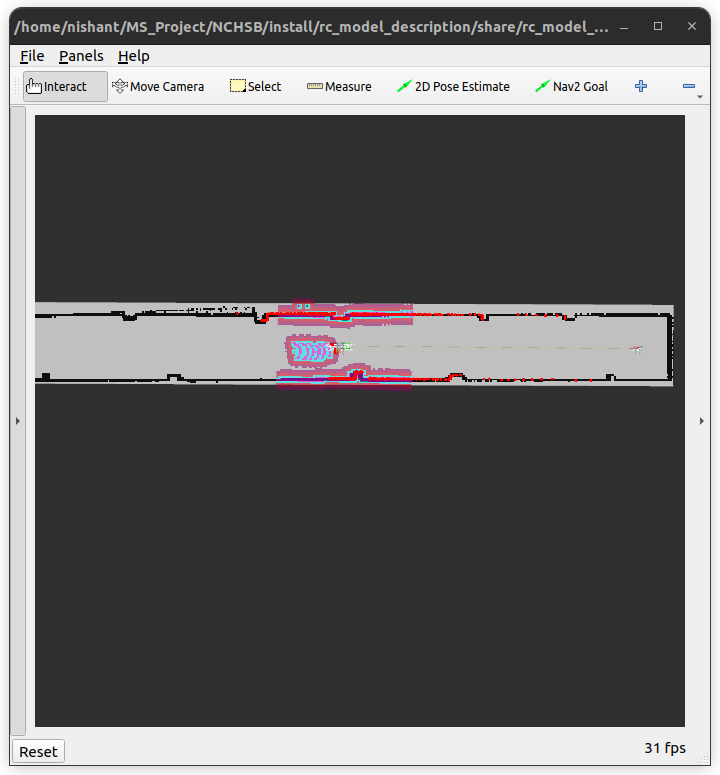
\includegraphics[width=0.48\textwidth]{day3_lidar_inflation_01.png}
  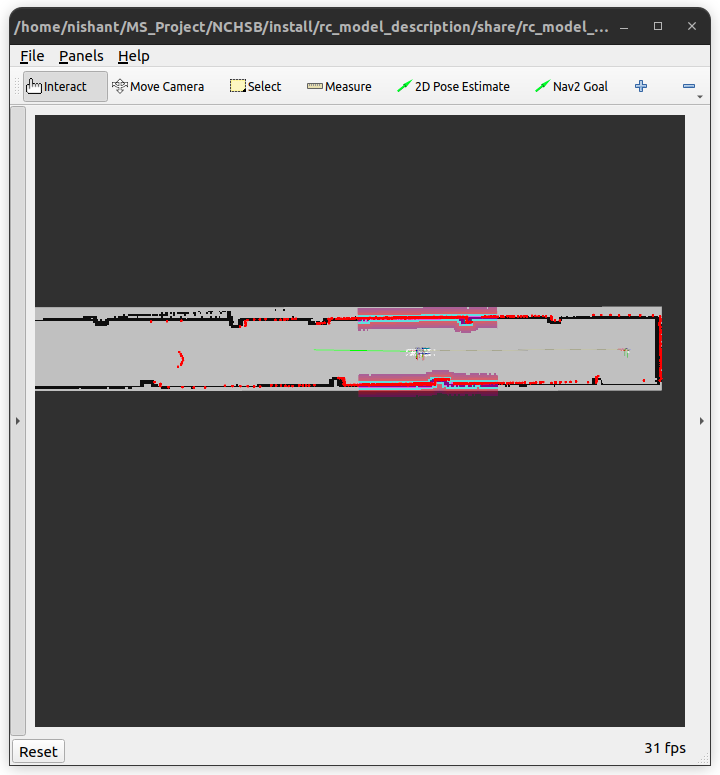
\includegraphics[width=0.48\textwidth]{day3_lidar_inflation_02.png}
  \caption{Day 3: LiDAR and inflation (1--2). Red points = obstacle layer,
    pink/purple = inflation. Pedestrian cylinder ahead of robot.}
\end{figure}

\begin{figure}[htbp]
  \centering
  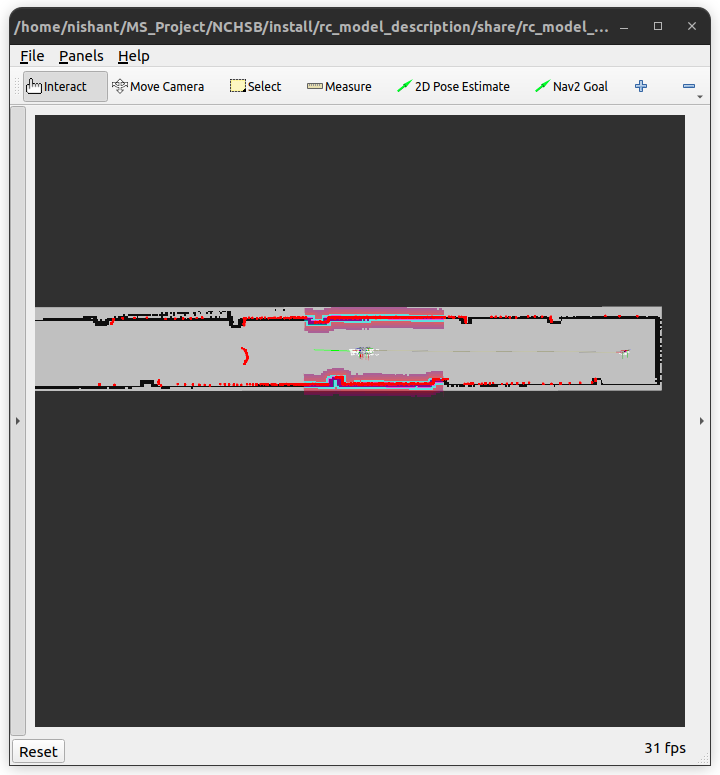
\includegraphics[width=0.48\textwidth]{day3_lidar_inflation_03.png}
  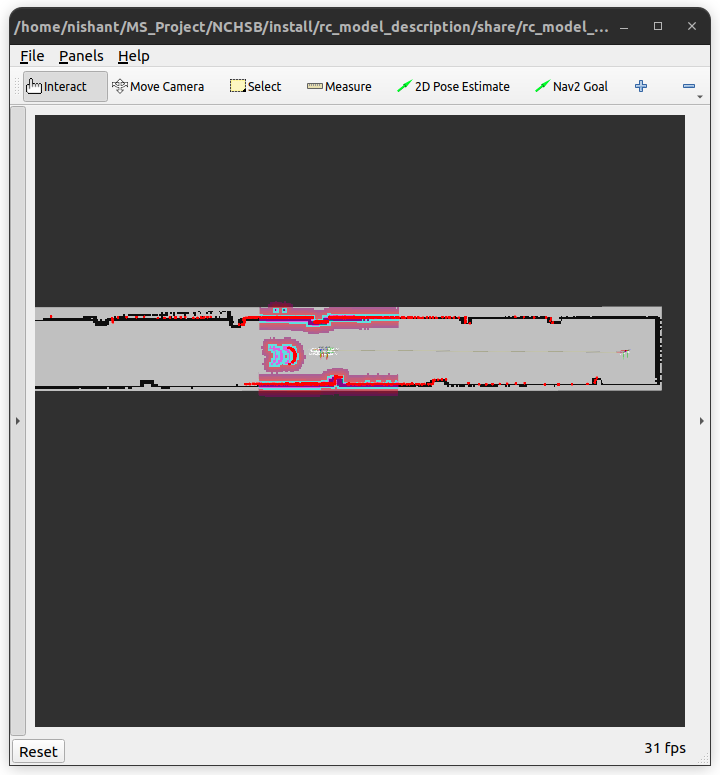
\includegraphics[width=0.48\textwidth]{day3_lidar_inflation_04.png}
  \caption{Day 3: LiDAR and inflation (3--4). Multiple red lines from moving
    pedestrian; inflation zone around cylinder.}
\end{figure}

\begin{figure}[htbp]
  \centering
  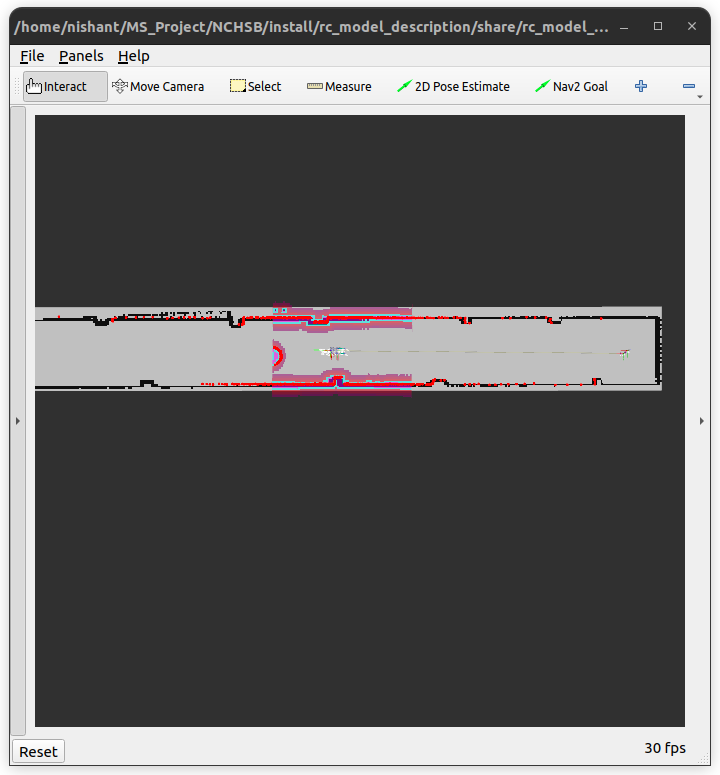
\includegraphics[width=0.48\textwidth]{day3_lidar_inflation_05.png}
  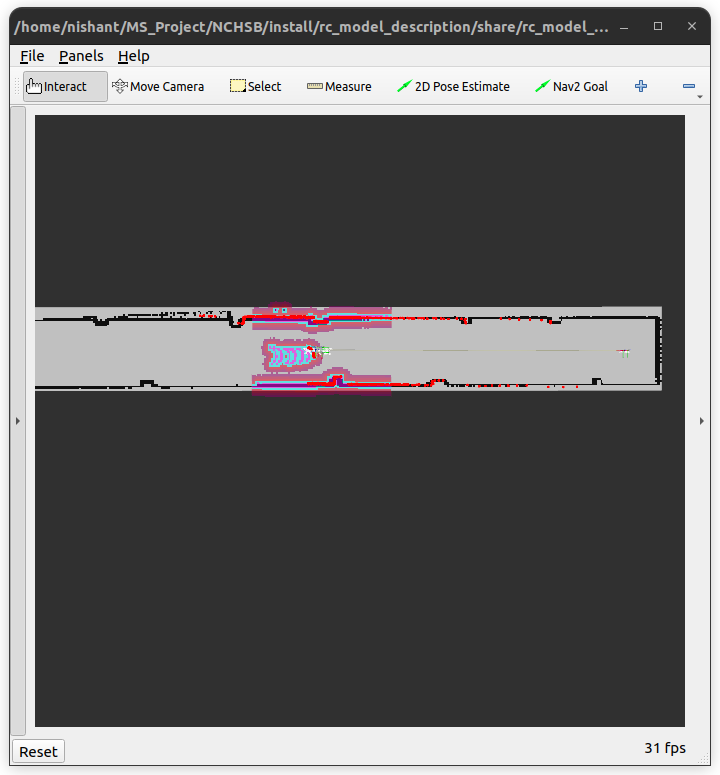
\includegraphics[width=0.48\textwidth]{day3_lidar_inflation_06.png}
  \caption{Day 3: LiDAR and inflation (5--6). Robot very close to inflation
    zone; screenshot before collision.}
\end{figure}

% ------------------------------------------------------------------

\subsection*{9.8 Day 3 Summary}

\logentry{Completed}
\begin{itemize}
  \item Priority 1: Robot motion verified (RViz ``reached'', odom confirms)
  \item Priority 2: Full trial completion (goal succeeded, CSV written)
  \item Priority 3: Pedestrian timing (signal-based) + physical movement
    (subprocess \texttt{ign service} instead of unbridged ROS service)
  \item Inflation radius: 0.09/0.08 $\to$ 0.25\,m in all 5 Nav2 configs
  \item Priority 4: Auto-shutdown implemented (on\_exit=Shutdown) --- but
    \textbf{unreliable}: Gazebo/RViz did not close; user had to Ctrl+C
\end{itemize}

\logentry{Remaining}
\begin{itemize}
  \item Priority 6: Smoke test all 4 controller configs (vanilla, social\_instant,
    social\_pred, full)
  \item Lateral offset distribution update (mean 0.35) --- not yet applied
  \item Fix auto-shutdown: launch process does not return to shell; investigate
    \texttt{Cannot shutdown a ROS adapter} exception
\end{itemize}

% ============================================================
\section{Day 4: Social Layer Architecture Rework}
% ============================================================

\logentry{External Review Analysis}
An external review (ChatGPT) of the social layer behavior identified the following
issues, largely confirming our internal diagnosis but correcting the proposed fix
approach:

\begin{enumerate}
  \item \textbf{Social cost appears too early}: Root cause is that
    \texttt{gt\_people\_publisher} is omniscient---it publishes all pedestrian
    poses from Gazebo GT regardless of LiDAR visibility or trial state.
    Combined with aggressive parameters (\texttt{amplitude: 252},
    \texttt{cutoff\_distance: 2.0}), the social blob fills half the corridor
    before the pedestrian is visually proximate.
  \item \textbf{Ghost/stale social costs (confirmed bug)}: The layer wrote
    directly into \texttt{master\_grid} with max-merge only. Old social cells
    were never cleared because:
    \begin{itemize}
      \item \texttt{updateBounds()} only expanded around \emph{current} person
        positions, not previous stamped regions.
      \item \texttt{reset()} only cleared \texttt{latest\_people\_}, not any
        cost state.
      \item There was no internal layer-owned map.
    \end{itemize}
  \item \textbf{Critical correction}: The initial fix proposal (``set old cells
    to FREE in \texttt{master\_grid}'') was \textbf{unsafe}---it would wipe
    costs from other layers (obstacle, static, inflation). Per Nav2 plugin
    guidelines, layers must maintain their own internal \texttt{costmap\_} and
    merge via \texttt{updateWithMax()}.
  \item \textbf{MPPI control-loop overruns}: Repeated
    ``\texttt{Control loop missed its desired rate}'' and
    ``\texttt{Optimizer fail to compute path}'' indicate the controller was
    computationally overloaded with \texttt{batch\_size: 1500},
    \texttt{time\_steps: 40}, and \texttt{visualize: true}.
\end{enumerate}

\logentry{Architectural Fix: SocialLayer and PredictiveSocialLayer}
Both costmap layer plugins were reworked following the same pattern:

\begin{enumerate}
  \item \textbf{Changed base class}: \texttt{nav2\_costmap\_2d::Layer} $\to$
    \texttt{nav2\_costmap\_2d::CostmapLayer}. This provides access to
    \texttt{resizeMap()}, \texttt{setCost()}, \texttt{getCost()},
    \texttt{updateWithMax()}, and \texttt{resetMaps()}.
  \item \textbf{Added \texttt{matchSize()} override}: Resizes the internal
    costmap to match the master layered costmap dimensions.
  \item \textbf{Reworked \texttt{updateCosts()}}:
    \begin{itemize}
      \item Clear the internal layer map (\texttt{FREE\_SPACE}) in the update
        region
      \item Stamp Gaussian costs into the internal map only
      \item Merge into master via \texttt{updateWithMax(master\_grid, ...)}
    \end{itemize}
  \item \textbf{Previous-bounds tracking}: Store
    \texttt{prev\_min\_x/y/max\_x/y} each cycle. In \texttt{updateBounds()},
    union current person bounds with previous bounds, ensuring old stamped
    regions are revisited and cleared.
  \item \textbf{Stale-message timeout}: If no \texttt{/tracked\_people} update
    for $>$\texttt{stale\_timeout} (default 0.5\,s), the people state is
    cleared, causing the layer to produce zero social cost.
  \item \textbf{\texttt{reset()} now complete}: Clears
    \texttt{latest\_people\_}, \texttt{has\_prev\_bounds\_}, and calls
    \texttt{resetMaps()} to zero the internal costmap.
\end{enumerate}

\logentry{GT People Publisher Robustness}
\texttt{gt\_people\_publisher.py} updated with:
\begin{itemize}
  \item \textbf{Stale model pruning}: Models not updated within
    \texttt{stale\_timeout} (default 1.0\,s) are removed from the published
    set, preventing ghost people.
  \item \textbf{Trial gating}: New parameter \texttt{gate\_on\_trial\_active}
    (default \texttt{True}). When enabled, the publisher subscribes to
    \texttt{/trial\_active} and only begins publishing \texttt{TrackedPeople}
    after receiving the signal. This prevents omniscient social cost before
    the robot starts navigating.
\end{itemize}

\logentry{Parameter Tuning (First Test Point)}
Following the external review's recommended starting point (not my original
sigma=0.8 proposal):

\begin{center}
\begin{tabular}{lrr}
\toprule
\textbf{Parameter} & \textbf{Old Value} & \textbf{New Value} \\
\midrule
\multicolumn{3}{l}{\emph{SocialLayer (instantaneous)}} \\
\texttt{amplitude} & 252.0 & 160.0 \\
\texttt{gaussian\_sigma} & 0.5 & 0.45 \\
\texttt{cutoff\_distance} & 2.0 & 1.2 \\
\midrule
\multicolumn{3}{l}{\emph{PredictiveSocialLayer (pred + full configs)}} \\
\texttt{max\_cost} & 252.0 & 160.0 \\
\texttt{cutoff\_distance} & 4.0 & 2.0 \\
\midrule
\multicolumn{3}{l}{\emph{MPPI (all 4 configs)}} \\
\texttt{batch\_size} & 1500 & 1000 \\
\texttt{time\_steps} & 40 & 30 \\
\texttt{visualize} & true & false \\
\bottomrule
\end{tabular}
\end{center}

\noindent\textbf{Rationale}: \texttt{amplitude: 160} is high enough to
discourage MPPI from crossing the person's immediate vicinity but low enough
($<$\,LETHAL\_OBSTACLE/2) that MPPI can still find feasible trajectories around
it. Keeping \texttt{sigma} at 0.45 (close to original 0.5) avoids widening the
far-field cost. Reducing \texttt{cutoff\_distance} from 2.0\,m to 1.2\,m
(instantaneous) and 4.0\,m to 2.0\,m (predictive) prevents the Gaussian from
spanning the entire corridor width. MPPI load reduction addresses the observed
control-loop overruns.

\logentry{Smoke Test: Ghost Streak Still Visible}
After the architectural rework, two smoke tests were run with
\texttt{mppi\_social\_instant}. The ghost streak and a ``purple semicircle
outside the map'' were still visible. Metrics: \texttt{collision\_count=1},
\texttt{min\_separation=0.209m}, \texttt{stuck\_time=10.24s},
\texttt{time\_to\_goal=13.09s}.

\textbf{Root cause identified}: \emph{Rolling-window origin mismatch}.
The internal \texttt{CostmapLayer} map had its origin set once during
\texttt{matchSize()}, but for a rolling-window local costmap the master grid's
origin shifts every cycle as the window follows the robot. Our code called
\texttt{mapToWorld(i, j, wx, wy)} on the \emph{internal} map (stale origin),
so the Gaussian was stamped at wrong world coordinates---producing ghost trails
at shifted positions and semicircles at map boundaries.

\textbf{Fix}: Changed \texttt{mapToWorld()} calls in \texttt{updateCosts()} to
\texttt{master\_grid.mapToWorld(i, j, wx, wy)}, since the cell indices
\texttt{(min\_i..max\_i)} are in the master grid's coordinate frame. Also added
a size-sync check at the top of \texttt{updateCosts()} for safety. Applied to
both \texttt{SocialLayer} and \texttt{PredictiveSocialLayer}.

\logentry{First Build Verification}
All three packages (\texttt{corridor\_social\_nav},
\texttt{corridor\_social\_nav\_bringup}, \texttt{rc\_model\_description})
rebuilt successfully with zero errors.

\logentry{Smoke Test After Architecture Rework --- Still Failing}
Ran two smoke tests with \texttt{mppi\_social\_instant} after the
\texttt{CostmapLayer} rework.

\textbf{Observations}:
\begin{itemize}
  \item Ghost streak still visible in RViz.
  \item Purple social cost sphere appeared \emph{disconnected} from the actual
    pedestrian position---not centered on the person.
  \item Social cost appeared as a purple semicircle at the edge of the map,
    partly outside the costmap boundaries.
  \item Metrics: \texttt{success=0}, \texttt{collision\_count=1},
    \texttt{min\_separation=0.154m}, \texttt{stuck\_time=11.5s}
\end{itemize}

\noindent\textbf{Hypothesis 1 (rolling-window origin mismatch)}: The internal
\texttt{CostmapLayer}'s origin is set once during \texttt{matchSize()} but the
rolling-window local costmap shifts its origin every cycle. Calling
\texttt{this->mapToWorld()} used the stale internal origin, producing wrong
world coordinates for the Gaussian. \textbf{Fix attempted}: Changed to
\texttt{master\_grid.mapToWorld(i, j, wx, wy)}.

\textbf{Result}: Did not fix the problem. Ghost streak and position mismatch
persisted.

\logentry{Root Cause Identified: TF Frame Mismatch}
After two failed attempts, the \emph{actual} root cause was identified:

\begin{itemize}
  \item \texttt{gt\_people\_publisher} publishes \texttt{TrackedPeople} with
    \texttt{header.frame\_id = ``map''}.
  \item The local costmap operates in the \texttt{odom} frame
    (\texttt{global\_frame: odom}).
  \item The social layer took \texttt{person.position.x/y} directly as world
    coordinates \textbf{without any TF transformation}, effectively mixing
    \texttt{map}-frame positions with \texttt{odom}-frame cell coordinates.
  \item The \texttt{map} $\to$ \texttt{odom} transform (published by AMCL)
    introduces a non-zero offset. The Gaussian was stamped at the
    \texttt{map}-frame position interpreted as \texttt{odom}-frame coordinates,
    causing the social blob to appear at a \emph{different physical location}
    than the actual person.
  \item This also explained:
    \begin{itemize}
      \item \textbf{Ghost streak}: As the \texttt{map}$\to$\texttt{odom}
        correction changed, old Gaussian stamps appeared at varying wrong
        positions.
      \item \textbf{Semicircle at map edge}: Wrong coordinates near costmap
        boundaries produced clipped artifacts.
      \item \textbf{``Social cost appears early''}: The social cost was
        physically present but at the wrong location, making it seem unrelated
        to the visible pedestrian.
    \end{itemize}
\end{itemize}

\noindent\textbf{Key insight}: All three previous ``bugs'' (ghost streak,
early appearance, semicircle) were \emph{symptoms of a single root cause}:
the missing TF transformation in the social layer.

\logentry{Fix: TF Transformation in Social Layers}
Both \texttt{SocialLayer} and \texttt{PredictiveSocialLayer} were updated:

\begin{enumerate}
  \item Added \texttt{tf2\_ros::Buffer} and \texttt{tf2\_ros::TransformListener}
    as class members, initialized in \texttt{onInitialize()}.
  \item Added \texttt{transformPeopleToGlobal()} method that:
    \begin{itemize}
      \item Reads the costmap's \texttt{global\_frame} (e.g., \texttt{odom})
      \item Looks up the TF from the people message's \texttt{frame\_id}
        (\texttt{map}) to the costmap's \texttt{global\_frame}
        (\texttt{odom})
      \item Transforms each person's position (and velocity, for the predictive
        layer) using \texttt{tf2::doTransform()}
      \item Short-circuits if \texttt{source\_frame == global\_frame}
      \item Logs a throttled warning if the transform is unavailable
    \end{itemize}
  \item \texttt{updateBounds()} now uses the \emph{transformed} positions for
    bounds expansion.
  \item \texttt{updateCosts()} stamps Gaussians using the \emph{transformed}
    positions, which are now in the costmap's native coordinate frame.
  \item Added \texttt{tf2\_geometry\_msgs} dependency to both targets in
    \texttt{CMakeLists.txt}.
  \item Added startup log line showing \texttt{global\_frame} to confirm the
    layer knows which frame it's operating in.
\end{enumerate}

\logentry{Summary of All Social Layer Fix Attempts (Chronological)}
\begin{center}
\begin{tabular}{|c|p{5cm}|p{4cm}|c|}
\hline
\textbf{\#} & \textbf{What was tried} & \textbf{Why it didn't work} & \textbf{Correct?} \\
\hline
1 & Lower amplitude (252$\to$160), increase sigma (0.5$\to$0.8) &
    Treats symptom (cost too high) but not cause (wrong position) & Partial \\
\hline
2 & \texttt{CostmapLayer} rework: internal map + \texttt{updateWithMax()} &
    Correct architecture but ghost persisted because coordinates were still wrong & Correct arch. \\
\hline
3 & Previous-bounds tracking for ghost clearing &
    Old bounds were in wrong frame too & Correct idea \\
\hline
4 & Stale-message timeout (0.5\,s) &
    Orthogonal improvement, doesn't fix position & Useful \\
\hline
5 & GT publisher gating on \texttt{/trial\_active} &
    Good fix for ``appears early'' but doesn't fix position & Useful \\
\hline
6 & \texttt{master\_grid.mapToWorld()} instead of \texttt{this->mapToWorld()} &
    Fixes one coordinate issue but the \emph{person} coordinates were still in wrong frame & Partial \\
\hline
7 & \textbf{TF transform (map $\to$ odom)} &
    \textbf{Fixes the actual root cause} & \textbf{Root fix} \\
\hline
\end{tabular}
\end{center}

\noindent Parameters adjusted per external review (amplitude=160,
sigma=0.45, cutoff=1.2 for instant; max\_cost=160, cutoff=2.0 for
predictive). MPPI load reduced (batch\_size 1500$\to$1000,
time\_steps 40$\to$30, visualize=false) across all configs.

\logentry{Smoke Test After TF Fix --- Still Wrong Position}
Even with TF transformation in the social layer, the purple social cost sphere
appeared disconnected from the pedestrian and ``before the cylinder comes.''
No \texttt{cannot transform} warnings in the log, so the TF lookup was
succeeding. But the \emph{transform itself was wrong}.

\textbf{Root cause}: AMCL's \texttt{initial\_pose} was hardcoded to
\texttt{(0, 0, 0)} in every Nav2 YAML config, while the robot spawns at
\texttt{(-9, 0, 0)}. The launch file passed \texttt{spawn\_x}/\texttt{spawn\_y}
to Gazebo for robot spawning but \textbf{never overrode AMCL's initial pose}.

With \texttt{initial\_pose = (0,0,0)} and robot spawning at \texttt{(-9, 0)}:
\begin{itemize}
  \item AMCL publishes a \texttt{map$\to$odom} transform that places the robot
    at \texttt{map(0,0)} instead of \texttt{map(-9, 0)}
  \item This \textasciitilde9\,m offset corrupts every \texttt{map$\to$odom}
    transformation
  \item The social layer's TF lookup succeeds but returns wrong coordinates,
    placing the Gaussian at $\sim$9\,m from the actual pedestrian position
  \item AMCL eventually converges toward the correct pose via scan matching,
    but the initial error is large and slow to correct
\end{itemize}

\logentry{Fix: Patch AMCL Initial Pose at Launch Time}
Modified \texttt{sim\_experiment.launch.py}'s \texttt{\_build\_nav2\_launch()}
to:
\begin{enumerate}
  \item Read the Nav2 params YAML file
  \item Override \texttt{amcl.ros\_\_parameters.initial\_pose} with the actual
    \texttt{spawn\_x}, \texttt{spawn\_y}, \texttt{spawn\_yaw} values
  \item Write to a temporary patched YAML file
  \item Pass the patched file to \texttt{nav2\_bringup}
\end{enumerate}

This ensures AMCL's initial \texttt{map$\to$odom} transform is correct from
the very first frame, regardless of which corridor or spawn position is used.

\logentry{Updated Fix Attempt Summary}
\begin{center}
\begin{tabular}{|c|p{5cm}|p{4cm}|c|}
\hline
\textbf{\#} & \textbf{What was tried} & \textbf{Why it didn't work} & \textbf{Correct?} \\
\hline
1 & Lower amplitude, adjust sigma & Treats symptom, not cause & Partial \\
\hline
2 & \texttt{CostmapLayer} + \texttt{updateWithMax()} & Correct architecture, wrong coords & Correct \\
\hline
3 & Previous-bounds tracking & Old bounds in wrong frame & Correct \\
\hline
4 & Stale-message timeout & Orthogonal improvement & Useful \\
\hline
5 & GT publisher gating on \texttt{/trial\_active} & Good, doesn't fix position & Useful \\
\hline
6 & \texttt{master\_grid.mapToWorld()} & Partial fix for rolling window & Partial \\
\hline
7 & TF transform (map $\to$ odom) & Transform itself was wrong because AMCL initial pose was wrong & Root fix \\
\hline
8 & \textbf{Patch AMCL initial\_pose = spawn coords} & \textbf{Fixes the TF so fix \#7 works correctly} & \textbf{Root fix} \\
\hline
\end{tabular}
\end{center}

\logentry{Fix \#8 Broke Everything: yaml.dump Corrupted Nav2 Config}
The \texttt{yaml.safe\_load()} + \texttt{yaml.dump()} approach completely
reformatted the Nav2 YAML file, likely corrupting parameter types (e.g.,
\texttt{True}$\to$\texttt{true}), string-quoted arrays (footprint), and
numeric formatting. Result: on launch, the map and robot appeared at completely
different positions in RViz---the robot was $\sim$9\,m to the right of the map.
Nav2 was essentially broken by the reformatted config.

\textbf{Fix \#9}: Replaced \texttt{yaml.dump()} with targeted \texttt{re.sub()}
regex replacements that only modify the \texttt{initial\_pose} values
(\texttt{x}, \texttt{y}, \texttt{yaw}) while leaving the rest of the YAML file
byte-for-byte identical. The patched file is written to a temporary file and
passed to \texttt{nav2\_bringup}.

Regex verified: correctly transforms
\texttt{initial\_pose: x: 0.0} $\to$ \texttt{initial\_pose: x: -9.0} without
affecting any other content.

\logentry{Updated Fix Attempt Summary (Final)}
\begin{center}
\begin{tabular}{|c|p{5cm}|p{4cm}|c|}
\hline
\textbf{\#} & \textbf{What was tried} & \textbf{Result} & \textbf{Status} \\
\hline
1 & Lower amplitude, adjust sigma & Treats symptom, not cause & Partial \\
\hline
2 & \texttt{CostmapLayer} + \texttt{updateWithMax()} & Correct architecture & Kept \\
\hline
3 & Previous-bounds tracking & Correct idea & Kept \\
\hline
4 & Stale-message timeout & Orthogonal improvement & Kept \\
\hline
5 & GT publisher gating on \texttt{/trial\_active} & Prevents early publish & Kept \\
\hline
6 & \texttt{master\_grid.mapToWorld()} & Rolling window fix & Kept \\
\hline
7 & TF transform (map $\to$ odom) & Root fix for coordinates & Kept \\
\hline
8 & AMCL initial\_pose via yaml.dump & \textbf{BROKE Nav2 config} & Reverted \\
\hline
9 & \textbf{AMCL initial\_pose via regex} & \textbf{Targeted text replace} & \textbf{Current} \\
\hline
\end{tabular}
\end{center}

\logentry{Smoke Test 9 Results (mppi\_social\_instant\_log4)}
The regex-based AMCL initial pose patching (Fix \#9) worked---AMCL log confirms
\texttt{Setting pose: -9.000 0.000 0.000}. However, the robot was \emph{still}
non-functional:
\begin{itemize}
  \item \textbf{Error}: ``\texttt{Robot is out of bounds of the costmap!}'' and
        ``\texttt{Start pose is out of costmap!}'' from the planner, repeated
        continuously.
  \item The SmacPlanner never computed a path; the goal feedback showed
        \texttt{0.00m remaining} (default/uninitialized value).
  \item The robot did not move at all.
  \item \textbf{Positive}: The social layer TF transform fix \emph{was} working
        --- the purple cost sphere correctly tracked the pedestrian cylinder.
\end{itemize}

\logentry{Root Cause: Map Origin Did Not Include Robot Spawn Position (Fix \#10)}
The SLAM-generated map \texttt{corridor\_straight.yaml} had:
\begin{verbatim}
origin: [-0.982, -1.25, 0]
\end{verbatim}
This corresponds to a map X range of $-0.98$ to $+19.27$\,m. The robot spawns
at $x = -9.0$ in Gazebo world coordinates, which is \textbf{outside the map bounds}.

\textbf{Explanation}: During SLAM mapping, the robot started at \texttt{odom(0, 0)},
which corresponded to Gazebo world position $(-9, 0)$. The resulting map uses odom
coordinates, so the corridor spans $x \in [-0.98, 19.27]$ in the map frame. But the
scenario files specify spawn and goal in \emph{Gazebo world coordinates} ($x = -9$
and $x = 9$). The AMCL initial pose was now correctly set to $(-9, 0)$ --- but this
point was outside the map, so the planner could not find the robot.

\textbf{Fix}: Shift the map origin by the robot's Gazebo spawn offset so that map
coordinates align with Gazebo world coordinates:
\begin{verbatim}
origin: [-9.982, -1.25, 0]    (was: [-0.982, -1.25, 0])
\end{verbatim}
New map X range: $-9.98$ to $+10.27$\,m. Both spawn $(-9, 0)$ and goal $(9, 0)$
are now inside the map.

Applied the same fix to all active corridor maps:
\begin{itemize}
  \item \texttt{corridor\_doorway.yaml}: $(-0.976, -2.5) \to (-6.976, -2.5)$
        (spawn $x = -6.0$)
  \item \texttt{corridor\_tjunction.yaml}: $(-1.48, -1.04) \to (-7.98, -1.04)$
        (spawn $x = -6.5$)
\end{itemize}

\logentry{Updated Fix Attempt Summary (Day 5)}
\begin{center}
\begin{tabular}{|c|p{5cm}|p{4cm}|c|}
\hline
\textbf{\#} & \textbf{What was tried} & \textbf{Result} & \textbf{Status} \\
\hline
1--6 & Social layer architecture fixes & See Day 4 log & Kept \\
\hline
7 & TF transform (map $\to$ odom) & Root fix for coordinates & Kept \\
\hline
8 & AMCL initial\_pose via yaml.dump & BROKE Nav2 config & Reverted \\
\hline
9 & AMCL initial\_pose via regex & Correct, but map too small & Kept \\
\hline
10 & \textbf{Shift map origin to align with Gazebo world} & \textbf{Spawn \& goal inside map} & \textbf{Current} \\
\hline
\end{tabular}
\end{center}

\logentry{Files Changed (Fix \#10)}
\begin{enumerate}
  \item \texttt{src/rc\_model\_description/maps/corridor\_straight.yaml} --- origin shifted by $-9.0$ in $x$
  \item \texttt{src/rc\_model\_description/maps/corridor\_doorway.yaml} --- origin shifted by $-6.0$ in $x$
  \item \texttt{src/rc\_model\_description/maps/corridor\_tjunction.yaml} --- origin shifted by $-6.5$ in $x$
\end{enumerate}
Packages \texttt{rc\_model\_description} and
\texttt{corridor\_social\_nav\_bringup} rebuilt successfully.

\logentry{Smoke Test 10: Map Aligned but Robot Did Not Evade (Fix \#10 Verified)}
After applying Fix \#10, the SLAM map, costmap, LiDAR, and social cost sphere all
aligned correctly. The robot navigated and received valid paths from the planner.
\textbf{However}, the robot drove straight through the pedestrian's social cost zone
without slowing down or deviating. Collision detected at $d = 0.395$\,m.

\textbf{Root Cause}: MPPI critic weight imbalance. The \texttt{ObstaclesCritic}
(weight 10.0) read social costs of $160/252 \approx 6.35$ per timestep, but the
\texttt{PathAlignCritic} (weight 15.0) and \texttt{GoalCritic} (weight 8.0) pulled
the robot rigidly along the planned path through the corridor center. In a $\sim$2\,m
wide corridor, ALL trajectory samples hit similar social costs, so MPPI could not
distinguish avoidance alternatives.

\logentry{Fix \#11: MPPI Social Tuning for Corridor Avoidance}
Parameter changes to \texttt{nav2\_mppi\_social\_instant.yaml}:
\begin{center}
\begin{tabular}{|l|c|c|p{5cm}|}
\hline
\textbf{Parameter} & \textbf{Old} & \textbf{New} & \textbf{Rationale} \\
\hline
social\_layer amplitude & 160 & 252 & Near-max costmap cost; the social zone now
dominates \\
\hline
social\_layer cutoff\_distance & 1.2\,m & 2.5\,m & Robot sees cost gradient earlier,
wider lateral gradient in corridor \\
\hline
social\_layer gaussian\_sigma & 0.45 & 0.5 & Slightly wider spread for smoother
gradient \\
\hline
ObstaclesCritic cost\_weight & 10 & 25 & 2.5$\times$ boost so social costs dominate
path critics \\
\hline
ObstaclesCritic critical\_weight & 30 & 40 & Stronger penalty for near-inscribed
costs \\
\hline
ObstaclesCritic collision\_margin & 0.15 & 0.20 & Slightly larger safety buffer \\
\hline
PathAlignCritic cost\_weight & 15 & 8 & Reduced rigidity so MPPI can deviate from
path center \\
\hline
inflation\_radius (local) & 0.25 & 0.35 & More wall clearance, gives robot room to
deviate \\
\hline
\end{tabular}
\end{center}

\textbf{Expected behavior}: With these changes, the per-timestep social cost from the
\texttt{ObstaclesCritic} becomes $252/252 \times 25.0 = 25.0$ at the pedestrian
center, vs.\ $\sim$8.0 for path deviation. MPPI should strongly prefer trajectories
that slow down or hug the wall. The wider cutoff provides an asymmetric cost gradient
across the corridor width, enabling wall-hugging rather than center-tracking.

\logentry{Smoke Test 11: Social Costs Still Ignored (Fix \#11 Failed)}
Result: Collision at $d = 0.446$\,m, \texttt{path\_length\_m} = 8.478\,m. Robot
navigated the full corridor but did not avoid the pedestrian.

\textbf{Root cause}: Wrong MPPI parameter name.  The \texttt{ObstaclesCritic}
initialization log reads:
\begin{verbatim}
ObstaclesCritic instantiated with 1 power and 40.000000 / 1.500000 weights
\end{verbatim}
The second number (\texttt{1.5}) is the \textbf{repulsion\_weight}, which was still
at its default because the YAML used \texttt{cost\_weight: 25.0} --- but
Nav2 Humble's MPPI \texttt{ObstaclesCritic} reads
\texttt{repulsion\_weight}, not \texttt{cost\_weight}. The base
\texttt{CriticFunction} class defines \texttt{cost\_weight} but it is
\emph{not} the field used in the non-lethal cost calculation.

With \texttt{repulsion\_weight = 1.5} (default), each timestep social cost was only
$252 \times 1.5 / 252 = 1.5$---easily overpowered by path-following critics.

\logentry{Fix \#12: Correct Parameter Name + Visual Debugging}
\begin{enumerate}
  \item Changed \texttt{cost\_weight: 25.0} to \texttt{repulsion\_weight: 30.0} in
        \texttt{ObstaclesCritic} section. Per-timestep cost now:
        $252 \times 30.0 / 252 = 30.0$.
  \item Enabled \texttt{visualize: true} in MPPI to show candidate trajectories in
        RViz.
  \item Added \texttt{/local\_plan} (magenta) path display to
        \texttt{urdf.rviz}.
  \item Added \texttt{/local\_plan\_trajectories} (MPPI MarkerArray) display.
  \item Added \texttt{GlobalCostmap} display (disabled by default, can toggle).
\end{enumerate}

\textbf{Expected log confirmation}:
\begin{verbatim}
ObstaclesCritic instantiated with 1 power and 40.000000 / 30.000000 weights
\end{verbatim}

\logentry{Smoke Test 12: Wheels Turning, No Lateral Motion (Fix \#12 Confirmed)}
The \texttt{ObstaclesCritic} log now reads \texttt{40.0 / 30.0} (was \texttt{1.5}).
MPPI IS commanding steering (user observed wheels turning). However, the robot did
not actually move laterally. Collision at $d = 0.395$\,m. 384 control loop misses from
\texttt{visualize: true}.

\textbf{Root cause}: Ackermann kinematics requires forward velocity for steering to
produce lateral displacement. With \texttt{vx\_min = 0.0}, MPPI generates
``stop-and-steer'' trajectories: high social cost $\Rightarrow$ near-zero forward
speed, so steering rotates the wheels but produces no lateral motion. This matches
the user's teleop observation: keys \texttt{u}/\texttt{o} (forward+turn) work, but
\texttt{j}/\texttt{l} (pure rotation) do nothing on Ackermann.

\logentry{Fix \#13: Minimum Forward Velocity + Performance Recovery}
\begin{enumerate}
  \item \texttt{vx\_min: 0.0 $\to$ 0.1} --- ensures MPPI always maintains forward
        crawl, so steering produces actual lateral displacement.
  \item \texttt{visualize: true $\to$ false} --- recovers controller performance
        (384 $\to$ $\sim$26 missed loops expected).
  \item Added \texttt{cmd\_vel\_logger} debug node to monitor MPPI's commanded
        velocities (\texttt{vx}, \texttt{vy}, \texttt{wz}) at 1\,Hz.
\end{enumerate}

\textbf{Files changed}:
\begin{itemize}
  \item \texttt{nav2\_mppi\_social\_instant.yaml}: vx\_min, visualize
  \item \texttt{cmd\_vel\_logger.py}: new debug node
  \item \texttt{setup.py}: registered cmd\_vel\_logger entry point
  \item \texttt{sim\_experiment.launch.py}: added cmd\_vel\_logger node
\end{itemize}

Ready for smoke test.

% ============================================================

\section*{Future Work / Nice-to-Haves}
\begin{itemize}
  \item \textbf{AWS RoboMaker Hospital World for visual fidelity}: The \texttt{aws-robomaker-hospital-world} (GitHub: \texttt{aws-robotics/aws-robomaker-hospital-world}) provides a detailed hospital environment with corridors, rooms, furniture, and human models. However:
    \begin{itemize}
      \item It targets Gazebo Classic (7.14+ / 9.16+), NOT Ignition Fortress --- incompatible plugin APIs.
      \item The ``humans'' are static mesh models (ElderLadyPatient, etc.), not moving pedestrians.
      \item Porting the full world is multi-day effort and out of scope.
    \end{itemize}
    \textbf{Middle ground}: Many furniture models (chairs, carts, cabinets) referenced in the hospital world are hosted on Ignition Fuel (\texttt{fuel.ignitionrobotics.org}) and work natively with Fortress. After the experiment pipeline is complete, 2--3 Fuel models can be placed in each corridor as static clutter for more realistic paper screenshots and additional SLAM features. This is cosmetic, not scientific --- the controlled geometric corridors are \emph{better} for a controls paper because confounding variables are minimized.
\end{itemize}

\end{document}
